% !TEX program = xelatex
\documentclass[12pt]{article}

\usepackage[a4paper, top=3cm, bottom=2cm, left=3cm, right=2cm]{geometry}

\usepackage[portuguese]{babel}
\usepackage{fontspec}
\usepackage{graphicx}
\graphicspath{{../}}
\usepackage{amsfonts}
\usepackage{amsmath}
\usepackage{amssymb}
\usepackage{mathtools}
\usepackage{indentfirst}
\usepackage{booktabs}
\usepackage{caption}
\usepackage{subcaption}
\usepackage{setspace}
\usepackage{fancyhdr}
\fancypagestyle{abnt}{
    \fancyhf{}
    \renewcommand{\headrulewidth}{0pt}
    \fancyhead[R]{\thepage}
}

\setlength{\parindent}{1.25cm}
\renewcommand{\baselinestretch}{1.5}

\setmainfont{Times New Roman}

\usepackage[round,authoryear,sort&compress]{natbib}

\PassOptionsToPackage{hyphens}{url}
\usepackage{hyperref}
\hypersetup{
    colorlinks=true,
    linkcolor=blue,
    filecolor=magenta,
    urlcolor=cyan,
    citecolor=red,
    pdftitle={Predição de Falhas em Turbinas Eólicas},
    pdfpagemode=UseOutlines,
}

\begin{document}
\begin{center}
\vspace*{1cm}
\Large
\textbf{Universidade Federal de São Paulo - UNIFESP}

\normalsize

Instituto de Ciência e Tecnologia - ICT

Bacharelado em Ciência e Tecnologia / Engenharia de Computação

\vspace*{\fill}

\Large

\textbf{Predição de Falhas em Turbinas Eólicas Utilizando Modelos de Aprendizado Profundo e Dados Exógenos}

\vspace{5mm}

\noindent\rule{\textwidth}{0.4pt}

\vspace{5mm}

\normalsize

Relatório Final de Iniciação Científica submetido à \\ Fundação de Amparo à Pesquisa do Estado de São Paulo (FAPESP).

\vspace{5mm}

\noindent\rule{\textwidth}{0.4pt}

\vspace{5mm}

\end{center}

\vspace*{\fill}

\normalsize

\vspace{0.5cm}

\begin{flushright}

\textbf{Aluno:} Thiago Solé Gomes Heleno

\textbf{Orientador:} Marcos G. Quiles

\textbf{Coorientador:} Mateus Giesbrecht (FEEC/Unicamp)

\vspace{10mm}

\centering \textbf{Vigência da Solicitação:} 01/06/2025 -- 31/05/2026

\end{flushright}

\vspace{5mm}

\begin{center}
São José dos Campos, maio de 2026
\end{center}

\newpage

% ─── Resumo (NBR 6028) ───────────────────────────────────────────────────────
\section*{Resumo}
\begin{singlespace}
\noindent
A energia eólica é peça-chave na transição para uma matriz energética limpa, mas sua viabilidade depende da operação contínua das turbinas. Falhas mecânicas e eletrônicas geram custos elevados de O\&M e perda de geração, motivando o uso de manutenção preditiva apoiada em dados SCADA (Supervisory Control and Data Acquisition). O presente projeto de Iniciação Científica investigou modelos de aprendizado profundo para detecção de anomalias em turbinas eólicas a partir do dataset público CARE\_To\_Compare (Wind Farm C, 3,18~M amostras de 10 minutos, 957 colunas (incluindo identificadores), razão Normal:Anomalia $\approx$ 51:1). O escopo original previa integração com dados meteorológicos exógenos (CPTEC/INPE, OpenWeatherMap), mas a anonimização total das coordenadas e datas absolutas no dataset inviabilizou essa fusão; o projeto foi readequado para comparar dois paradigmas alternativos --- supervisionado e não supervisionado --- e para explorar \textit{data augmentation} via injeção de falhas sintéticas. Foram implementados cinco notebooks: (i) CNN, LSTM e CNN-LSTM supervisionados (replicação de Qi et al., 2024); (ii) Autoencoder CNN-BiLSTM com camada de atenção em PyTorch; (iii) Autoencoder MLP em Keras com otimização Optuna e métrica CARE; (iv) classificador MLP de 3 classes com falhas induzidas; e (v) Autoencoder MLP com calibração de threshold por falhas induzidas. Os autoencoders não supervisionados atingiram AUC-ROC de até 0,872 (vs.\ 0,66 do melhor supervisionado), confirmando a vantagem do paradigma sob desbalanceamento severo, embora a precisão amostral baixa ($\sim$2--3\%) ainda inviabilize uso direto em produção. O CARE Score do NB3 (0,699) e a calibração induzida do NB5 (CARE 0,545 com Acc por evento de 0,98) sugerem \textit{ensembles} como linha futura natural.
\end{singlespace}

\vspace{0.5cm}
\noindent\textbf{Palavras-chave:} Turbinas Eólicas. Manutenção Preditiva. Aprendizado Profundo. Detecção de Anomalias. Autoencoder. SCADA. CARE Score.

\newpage

% ─── Listas (NBR 6027) ───────────────────────────────────────────────────────
\renewcommand{\contentsname}{Sumário}
\tableofcontents
\newpage
\listoffigures
\newpage
\listoftables
\newpage

% ─── Lista de Abreviaturas e Siglas ─────────────────────────────────────────
\section*{Lista de Abreviaturas e Siglas}
\begin{singlespace}
\noindent
\begin{tabular}{ll}
AE       & Autoencoder \\
AMP      & Automatic Mixed Precision \\
AUC-PR   & Area Under the Precision-Recall Curve \\
AUC-ROC  & Area Under the Receiver Operating Characteristic Curve \\
BiLSTM   & Bidirectional Long Short-Term Memory \\
CARE     & Composite Anomaly Reliability Evaluation \\
CNN      & Convolutional Neural Network \\
CNN1D    & Convolutional Neural Network 1D (temporal) \\
DL       & Deep Learning (Aprendizado Profundo) \\
EDA      & Exploratory Data Analysis (Análise Exploratória de Dados) \\
FN       & False Negative \\
FP       & False Positive \\
GPU      & Graphics Processing Unit \\
IC       & Iniciação Científica \\
LSTM     & Long Short-Term Memory \\
MAE      & Mean Absolute Error \\
ML       & Machine Learning (Aprendizado de Máquina) \\
MLP      & Multi-Layer Perceptron \\
MSE      & Mean Squared Error \\
NB       & Notebook \\
O\&M     & Operação e Manutenção \\
PReLU    & Parametric Rectified Linear Unit \\
ReLU     & Rectified Linear Unit \\
RMSE     & Root Mean Squared Error \\
RNN      & Recurrent Neural Network \\
SCADA    & Supervisory Control and Data Acquisition \\
SELU     & Scaled Exponential Linear Unit \\
TN       & True Negative \\
TP       & True Positive \\
TPU      & Tensor Processing Unit \\
WS       & Warning Score \\
\end{tabular}
\end{singlespace}
\newpage

% A partir da Introdução, a numeração aparece no canto superior direito
\pagestyle{abnt}

% ─── 1 INTRODUÇÃO ────────────────────────────────────────────────────────────
\section{Introdução}

% [Contextualização do tema, motivação, problema de pesquisa]
O aprendizado de máquina (ML) vem ganhando destaque como ferramenta essencial para melhorar a confiabilidade e a eficiência de sistemas industriais complexos, como é o caso das turbinas eólicas, trazendo novas perspectivas para as estratégias de manutenção preditiva. Modelos de ML conseguem analisar padrões temporais em dados operacionais (vibração, temperatura, rotação, etc.) e integrar variáveis externas, prevendo assim falhas com maior precisão. Indo além da simples detecção de anomalias, técnicas avançadas como as redes neurais profundas possibilitam modelar as interações dinâmicas entre componentes mecânicos e fatores ambientais, o que ajuda a antecipar cenários críticos que poderiam levar a paradas custosas. Essas abordagens não apenas diminuem custos operacionais, mas também favorecem a sustentabilidade energética ao minimizar desperdícios.  

Contudo, construir modelos preditivos robustos esbarra em desafios importantes ligados à disponibilidade e qualidade dos dados. Um dos maiores obstáculos é a escassez de bases públicas de dados SCADA extensas e bem rotuladas. Além disso, os conjuntos de dados disponíveis sofrem com um desbalanceamento severo: as falhas são eventos extremamente raros em comparação aos longos períodos de operação normal. Essa falta de amostras representativas de anomalias dificulta significativamente o treinamento, pois impede que os modelos de Redes Neurais aprendam adequadamente os padrões de falha, que por sua natureza já são altamente complexos e variáveis. A dificuldade de capturar informações em condições operacionais extremas acaba limitando a capacidade do modelo de generalizar eventos raros, comprometendo a escalabilidade e a confiabilidade das soluções propostas.  

Inicialmente, este projeto propunha o desenvolvimento de modelos preditivos combinando os dados operacionais da turbina com variáveis meteorológicas externas. Contudo, durante a execução da pesquisa, esbarrou-se em uma limitação técnica intrínseca aos dados abertos: os repositórios públicos anonimizam completamente a localização geográfica dos parques eólicos (fornecendo apenas identificadores genéricos) por questões de confidencialidade comercial. Sem as coordenadas exatas e datas absolutas, tornou-se impossível alinhar espacialmente e temporalmente os dados SCADA com bases meteorológicas externas (como CPTEC/INPE e OpenWeatherMap).  

Diante dessa inviabilidade, o escopo da pesquisa foi readequado. Em vez de comparar modelos com e sem dados exógenos, o projeto passou a focar na comparação entre diferentes paradigmas de detecção — supervisionado versus não supervisionado — e na exploração de técnicas alternativas para contornar a escassez de dados, como o uso de data augmentation via injeção de falhas sintéticas (induzidas). Como resultado, foram investigadas arquiteturas como CNN1D, LSTM e Autoencoders com mecanismos de atenção, e estabelecidos protocolos de avaliação para identificar a abordagem mais viável para o monitoramento de turbinas em cenários de dados escassos e desbalanceados.

% ─── 2 JUSTIFICATIVA ─────────────────────────────────────────────────────────
\section{Justificativa}
% [Relevância do projeto: redução de custos O&M, sustentabilidade, lacunas
%   na literatura, contribuição acadêmica]
Antecipar falhas em turbinas eólicas é fundamental para diminuir os custos com manutenções corretivas e evitar interrupções na geração de energia. A princípio, integrar dados meteorológicos aos modelos preditivos ajudaria a identificar padrões mais complexos, como o efeito de rajadas de vento ou de variações de temperatura no comportamento da máquina. No entanto, a realidade técnica dos repositórios de dados abertos — que ocultam a localização dos parques e carecem de amostras de falhas bem documentadas — evidencia uma lacuna crítica na pesquisa aplicada: a urgência de se criar modelos robustos que operem com alta precisão mesmo sob a escassez de dados anômalos e sem o apoio de variáveis climáticas externas.  

Nesse contexto, o projeto justifica-se fortemente pela necessidade de desenvolver soluções metodológicas que contornem essa restrição. Ao redirecionar o foco para a comparação entre métodos supervisionados e não supervisionados, e ao explorar técnicas como o data augmentation via injeção de falhas sintéticas, o trabalho busca aumentar a capacidade de generalização dos modelos de redes neurais quando submetidos a dados severamente desbalanceados.

Além de sua contribuição técnica, o uso de bases de dados públicas e de ferramentas de código aberto (como TensorFlow e PyTorch) favorece a acessibilidade e a reprodutibilidade do projeto, um ponto importante frente às demandas por transparência e sustentabilidade no setor energético. Por fim, a pesquisa mantém sua forte contribuição para o debate acadêmico sobre a aplicação do aprendizado de máquina industrial, trazendo insights práticos para aplicações em ambientes dinâmicos e propondo caminhos para viabilizar a manutenção preditiva diante de limitações reais na disponibilidade de dados.
% ─── 3 OBJETIVO ──────────────────────────────────────────────────────────────
\section{Objetivo}

\subsection{Aprendizado}

A vertente formativa deste projeto visou capacitar o aluno nos fundamentos teóricos e práticos necessários para a investigação proposta, com ênfase em aprendizado de máquina aplicado a séries temporais e em ferramentas computacionais para análise de dados SCADA. Esse eixo se desenvolveu em paralelo às atividades experimentais, com acompanhamento integral do \textbf{curso de Redes Neurais Artificiais ministrado pelo orientador Prof.\ Dr.\ Marcos G.\ Quiles}\footnote{Playlist disponível em: \url{https://www.youtube.com/watch?v=kzFqGhK8Q2s&list=PLxI8Can9yAHfB2om9dqhsrsjRAf-YJaro}.}, cujas vídeo-aulas e materiais de apoio estão organizados localmente em \texttt{aprendizado\_curso/}. Foram conduzidos exercícios práticos em PyTorch, NumPy e Pandas, replicando os blocos do curso antes de integrá-los aos pipelines do projeto.

\subsubsection{Fundamentos de Aprendizado de Máquina}

Estudo dos conceitos básicos de aprendizado supervisionado e não supervisionado: regressão, classificação binária e multi-classe, função de perda (MSE, MAE, Cross-Entropy), regularização ($L_1$, $L_2$, \textit{dropout}), divisão treino/validação/teste, validação cruzada e principais métricas de avaliação (acurácia, precisão, recall, F1, AUC-ROC, RMSE, MAE).

\subsubsection{Redes Neurais Artificiais}

Estudo do \textit{perceptron} simples, MLP (\textit{Multi-Layer Perceptron}), funções de ativação (ReLU, PReLU, SELU, Sigmoid, Softmax), \textit{backpropagation} via regra da cadeia, otimizadores baseados em gradiente (SGD, Adam, AdamW) e estratégias de inicialização (He, Xavier).

\subsubsection{Aprendizado Profundo}

Aprofundamento em redes recorrentes (RNN, LSTM, BiLSTM e seus \textit{gates} de \textit{input}, \textit{forget} e \textit{output}), redes convolucionais 1D (kernel, \textit{stride}, \textit{padding}, \textit{pooling}), mecanismos de atenção (\textit{scaled dot-product attention}, \textit{multi-head attention}), autoencoders e suas variantes (denso, convolucional, recorrente). O conteúdo foi acompanhado por exercícios práticos em PyTorch reproduzindo os blocos antes de integrá-los aos pipelines do projeto.

\subsection{Treinamento}

A etapa de treinamento contemplou tanto experimentação inicial em datasets reduzidos quanto a execução final dos cinco \textit{notebooks} sobre o Wind Farm C completo.

\subsubsection{Pipeline de Treinamento}

\begin{sloppypar}
O pipeline padrão adotado foi: (1) carregamento dos CSVs SCADA; (2) divisão treino/validação/teste (por evento no NB1 e NB4; temporal 70/15/15 dinâmico no NB2; coluna \texttt{train\_test} do CARE com sub-split 80/20 interno no NB3 e NB5 --- detalhes na Seção~\ref{subsec:validacao}); (3) pré-processamento (\textit{clipping} de outliers, imputação, normalização); (4) seleção de \textit{features}; (5) construção de janelas temporais quando aplicável; (6) treinamento com \textit{early stopping} sobre \textit{val\_loss}; (7) calibração de \textit{threshold} sobre validação; (8) avaliação no teste.
\end{sloppypar}

\subsubsection{Datasets de Aprendizado}

Antes da execução final no Wind Farm C, foram utilizados subconjuntos pequenos para validar a corretude dos pipelines e para fins didáticos: amostras balanceadas geradas a partir de poucos CSVs e datasets sintéticos de classificação binária do scikit-learn (\texttt{make\_classification}, \texttt{make\_moons}) para depurar funções de perda, otimizadores e callbacks de \textit{early stopping}.

% ─── 4 FUNDAMENTAÇÃO TEÓRICA ─────────────────────────────────────────────────
\section{Fundamentação Teórica}

\subsection{Manutenção Preditiva em Turbinas Eólicas}

A manutenção preditiva (\textit{Predictive Maintenance --- PdM}) busca antecipar falhas a partir do monitoramento contínuo da condição do equipamento, em contraste com a manutenção corretiva (após a falha) e a preventiva (em janelas fixas, independentes do estado real). Em turbinas eólicas, o custo das paradas não programadas é elevado, especialmente em parques \textit{offshore}, e a degradação dos componentes (caixa multiplicadora, rolamentos, gerador, sistema de \textit{pitch}) costuma evoluir gradualmente, deixando assinaturas detectáveis em sensores de vibração, temperatura e potência elétrica antes da falha. Esse cenário motiva a aplicação de técnicas de detecção de anomalias e prognóstico em séries temporais.

\subsection{Sistemas SCADA}

O sistema SCADA (\textit{Supervisory Control and Data Acquisition}) é a infraestrutura de monitoramento padrão de parques eólicos modernos, agregando dezenas a centenas de sensores instalados ao longo da turbina (nacele, rotor, hub, conversor, transformador). Os dados são tipicamente registrados em janelas de 10 minutos com agregações estatísticas (média, máximo, mínimo, desvio-padrão por janela), gerando um conjunto rico de variáveis (no Wind Farm C, 238 sensores físicos $\times$ 4 estatísticas = 957 colunas (incluindo identificadores)). Apesar de ser uma instrumentação menos precisa que sistemas dedicados de monitoramento de condição, sua disponibilidade ampla e baixo custo marginal tornam-no atrativo para algoritmos de aprendizado de máquina.

\subsection{Séries Temporais e Detecção de Anomalias}

Uma série temporal é uma sequência $\{x_t\}_{t=1}^{T}$ indexada pelo tempo. Em turbinas eólicas, cada sensor produz uma série multivariada com periodicidades (diurna, sazonal) e regimes operacionais (partida, geração nominal, parada). A detecção de anomalias busca identificar pontos ou subsequências cujo comportamento desvia significativamente do padrão observado. As três famílias principais de abordagens são: (i) baseadas em \textit{thresholds} estatísticos (Z-score, IQR); (ii) supervisionadas, treinando classificadores binários ou multi-classe sobre exemplos rotulados; (iii) não supervisionadas, treinando modelos para reconstruir ou prever o comportamento normal, e usando o erro de reconstrução/predição como \textit{score} de anomalia.

\subsection{Arquiteturas de Aprendizado Profundo}

\subsubsection{LSTM}

A LSTM (\textit{Long Short-Term Memory}) é uma RNN projetada para mitigar os problemas de gradiente desaparecente das RNNs tradicionais. Cada célula mantém um estado interno $C_t$ controlado por três \textit{gates}: \textit{forget gate} $f_t = \sigma(W_f[h_{t-1}, x_t] + b_f)$, \textit{input gate} $i_t = \sigma(W_i[h_{t-1}, x_t] + b_i)$ e \textit{output gate} $o_t = \sigma(W_o[h_{t-1}, x_t] + b_o)$. O estado é atualizado por $C_t = f_t \odot C_{t-1} + i_t \odot \tilde{C}_t$, onde $\tilde{C}_t = \tanh(W_C[h_{t-1}, x_t] + b_C)$, e a saída é $h_t = o_t \odot \tanh(C_t)$. A versão BiLSTM processa a sequência em ambas as direções e concatena os estados, capturando contexto passado e futuro. A Figura~\ref{fig:lstm} ilustra a estrutura interna da célula.

\begin{figure}[!ht]
    \centering
    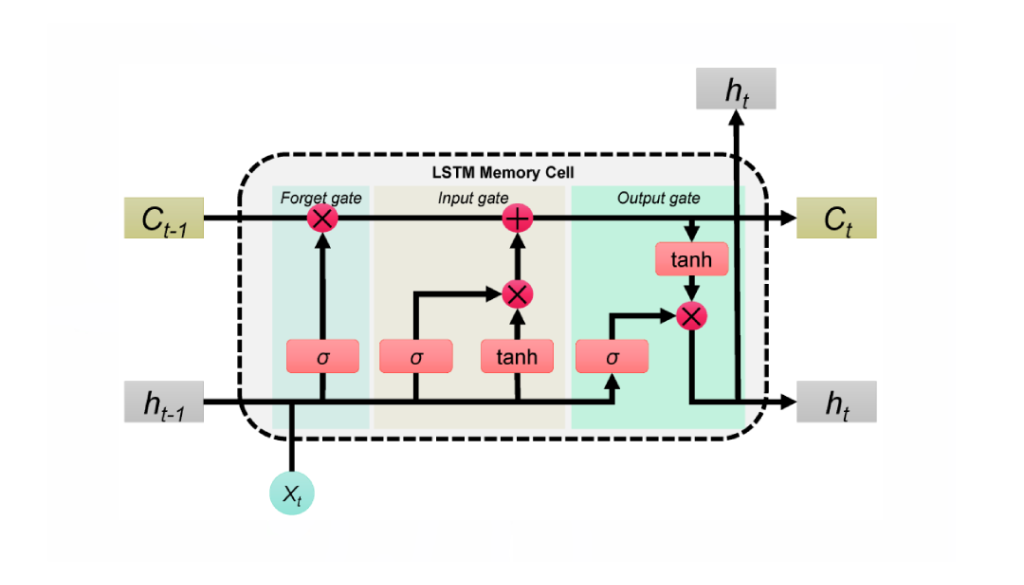
\includegraphics[width=0.75\textwidth]{figs/diagramas/lstm.png}
    \caption{Diagrama da célula LSTM com os três \textit{gates} (forget, input, output). Fonte: dida.do, ``Long Short-Term Memory Networks (LSTM): subtleties of mathematical inference'', \url{https://dida.do/blog/long-short-term-memory-network-lstm-subtleties-of-mathematical-inference}.}
    \label{fig:lstm}
\end{figure}

\subsubsection{CNN1D}

A CNN 1D aplica filtros convolucionais ao longo do eixo temporal: dado um sinal $x \in \mathbb{R}^{T \times C}$, um filtro $W \in \mathbb{R}^{k \times C}$ produz $y_t = \sum_{i=0}^{k-1} W_i x_{t+i} + b$. \textit{Stride} controla o passo entre janelas e \textit{padding} preserva o comprimento. Camadas de \textit{pooling} (max, avg) reduzem dimensionalidade temporal, e o empilhamento de várias camadas convolucionais aumenta o campo receptivo, permitindo que o modelo capte padrões em diferentes escalas temporais. A Figura~\ref{fig:cnn1d} mostra o diagrama de uma camada convolucional típica.

\begin{figure}[!ht]
    \centering
    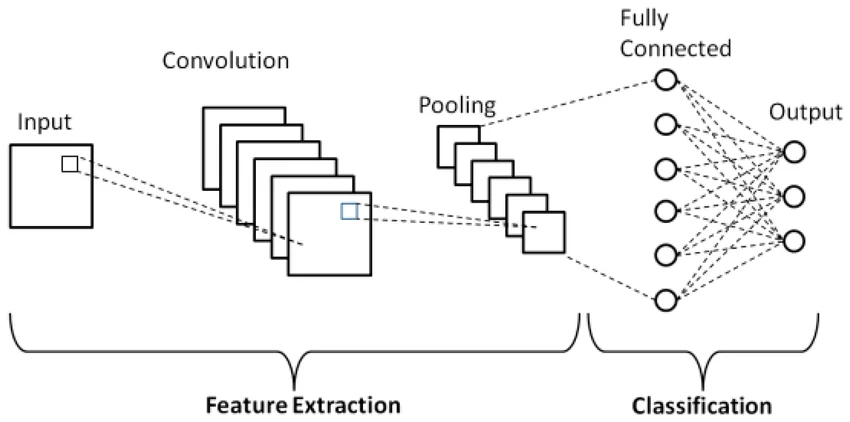
\includegraphics[width=0.7\textwidth]{figs/diagramas/cnn1d.png}
    \caption{Diagrama esquemático de uma rede convolucional (extração de \textit{features} via \textit{convolution}+\textit{pooling} seguida de classificação por camadas \textit{fully connected}). Fonte: \citet{Phung2019_CloudCNN}.}
    \label{fig:cnn1d}
\end{figure}

\subsubsection{MLP (\textit{Multi-Layer Perceptron})}

O MLP é uma rede totalmente conectada composta por uma camada de entrada, uma ou mais camadas ocultas e uma camada de saída. Cada neurônio aplica a transformação afim $z = Wx + b$ seguida de uma função de ativação não linear (PReLU nos NB3, NB4 e NB5). Na configuração autoencoder (NB3 e NB5), o MLP é treinado para reconstruir a própria entrada: o \textit{encoder} comprime o vetor de \textit{features} até um \textit{bottleneck} de dimensão reduzida (\texttt{code\_size}), e o \textit{decoder} simétrico reconstrói a entrada a partir dessa representação compacta. O erro de reconstrução (RMSE por amostra) é usado como \textit{score} de anomalia --- amostras fora do padrão normal aprendido exibem erro alto. A Figura~\ref{fig:mlp} ilustra a topologia do autoencoder MLP.

\begin{figure}[!ht]
    \centering
    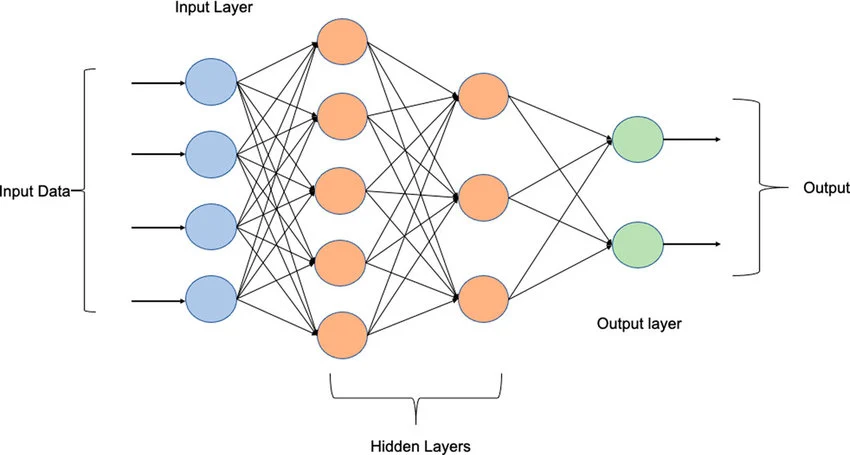
\includegraphics[width=0.55\textwidth]{figs/diagramas/mlp.png}
    \caption{Topologia genérica de um \textit{Multi-Layer Perceptron} (camada de entrada, camadas ocultas e camada de saída totalmente conectadas), arquitetura base do encoder/decoder dos autoencoders MLP utilizados nos NB3 e NB5. Fonte: \citet{Afan2021_Groundwater}.}
    \label{fig:mlp}
\end{figure}

\subsubsection{Mecanismo de Atenção (MultiHeadAttention)}

A atenção de produto-escalar escalado calcula $\mathrm{Attention}(Q, K, V) = \mathrm{softmax}\left(\frac{QK^\top}{\sqrt{d_k}}\right)V$, onde $Q$, $K$, $V$ são projeções lineares da entrada (\textit{queries}, \textit{keys}, \textit{values}). A versão \textit{multi-head} executa $h$ atenções paralelas em sub-espaços diferentes e concatena os resultados, permitindo que o modelo combine padrões em múltiplos pontos da sequência simultaneamente. \textbf{Importante:} no NB2 deste projeto, a atenção é utilizada como uma \textit{camada} dentro de uma arquitetura CNN-BiLSTM, e \textbf{não} como Transformer completo (não há \textit{positional encoding} explícito nem blocos \textit{encoder/decoder} no padrão original de \citet{Vaswani2017}). Essa distinção é importante em relação ao plano original, que previa Transformers completos. A Figura~\ref{fig:transformer} apresenta a arquitetura Transformer completa para referência conceitual.

\begin{figure}[!ht]
    \centering
    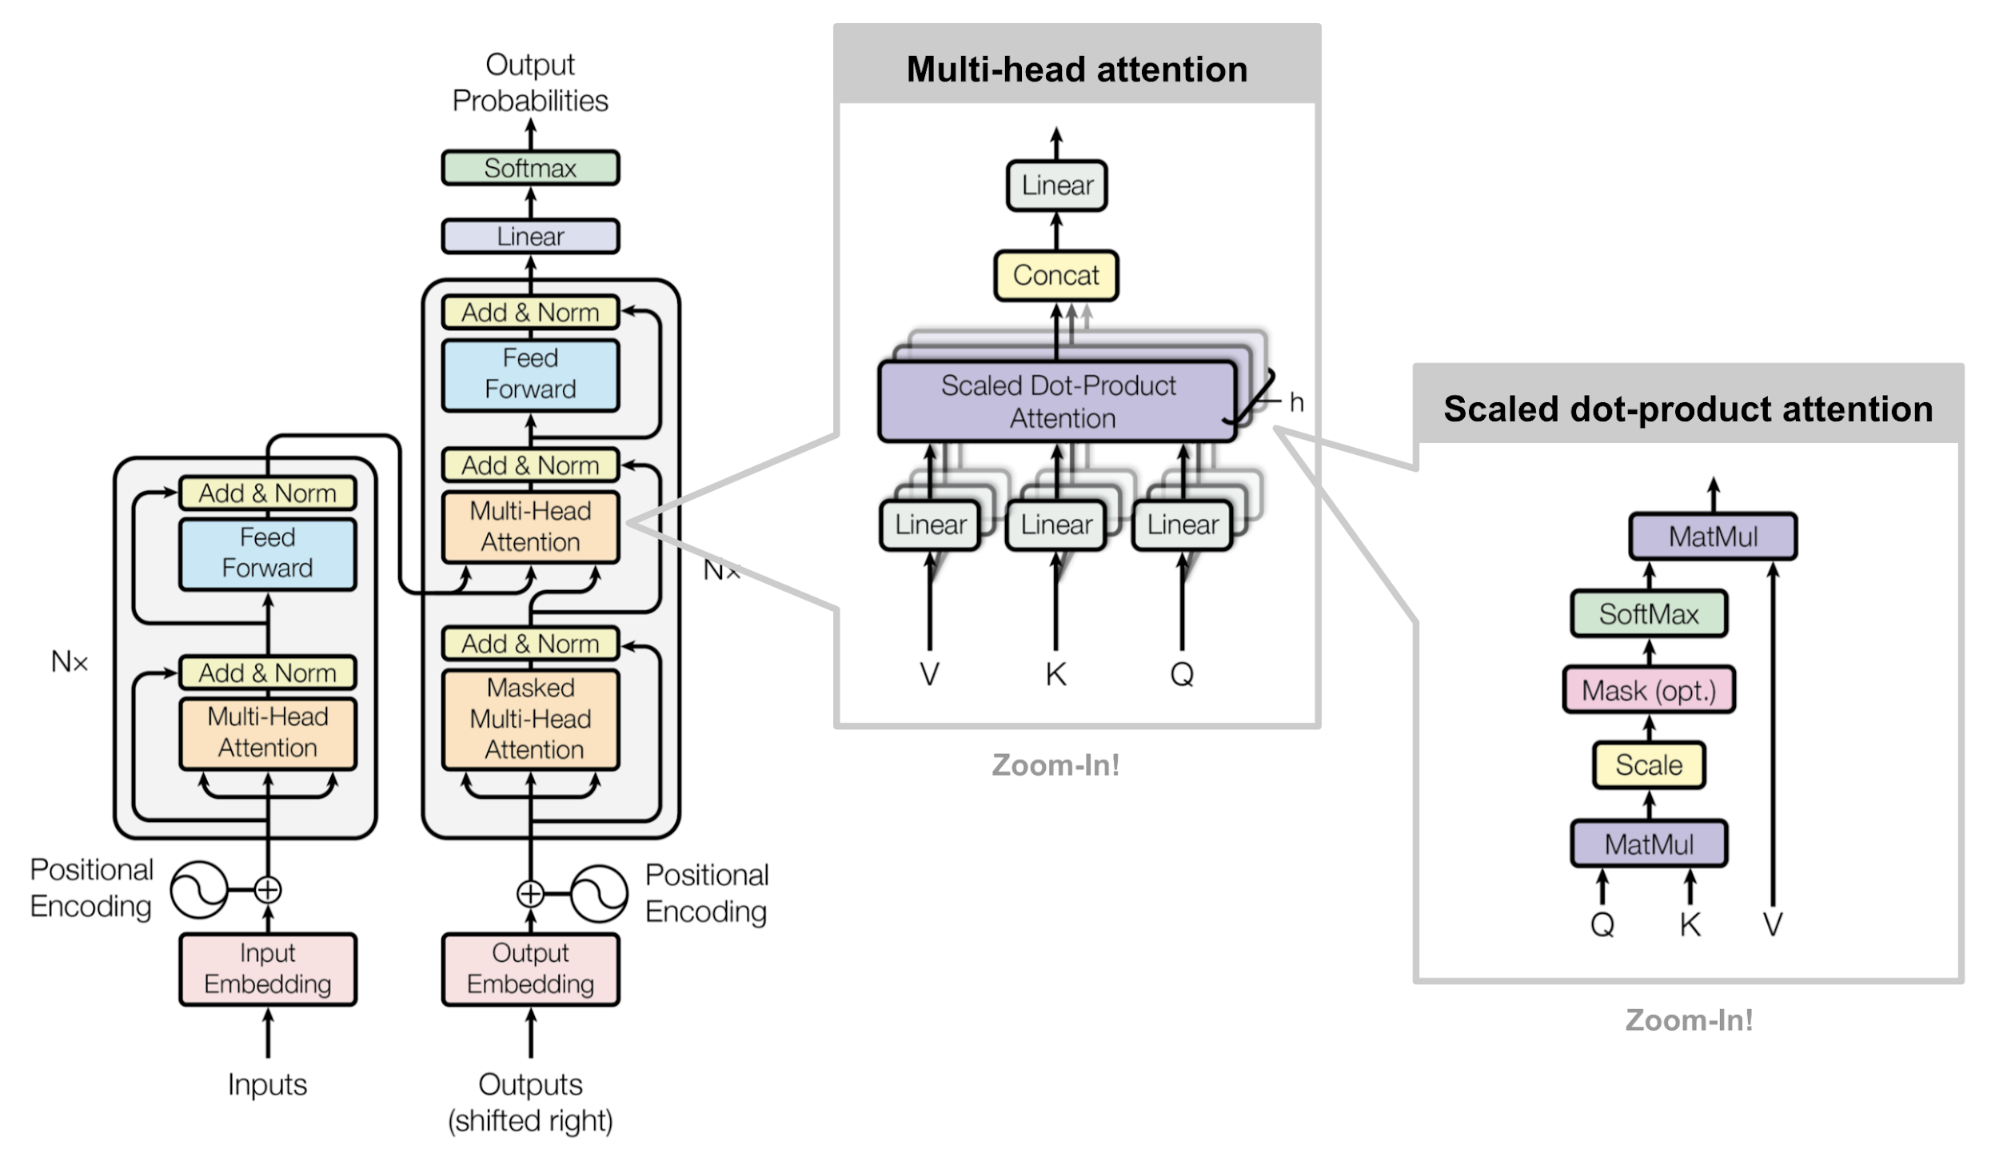
\includegraphics[width=0.55\textwidth]{figs/diagramas/transformer.png}
    \caption{Arquitetura Transformer completa (\textit{encoder/decoder} com \textit{multi-head attention} e \textit{positional encoding}), com \textit{zoom} em \textit{multi-head attention} e \textit{scaled dot-product attention}. Apenas a camada \texttt{MultiHeadAttention} foi utilizada neste projeto, dentro do encoder do NB2. Fonte: adaptado de \citet{Vaswani2017}.}
    \label{fig:transformer}
\end{figure}

\subsection{Métricas de Avaliação}

\subsubsection{Métricas Padrão de Classificação}

Sejam $TP$, $TN$, $FP$, $FN$ as entradas da matriz de confusão. Define-se:
\begin{align}
\mathrm{Acuracia}    &= \frac{TP + TN}{TP + TN + FP + FN}, &
\mathrm{Precisao}    &= \frac{TP}{TP + FP}, \\
\mathrm{Revocacao}   &= \frac{TP}{TP + FN}, &
F_1                  &= \frac{2 \cdot P \cdot R}{P + R}, \\
F_\beta              &= \frac{(1 + \beta^2) \cdot P \cdot R}{\beta^2 \cdot P + R}.
\end{align}
A AUC-ROC é a área sob a curva ROC (TPR $\times$ FPR), independente de \textit{threshold}, e mede a qualidade do ordenamento dos \textit{scores}. Em datasets fortemente desbalanceados, a AUC-PR (área sob a curva Precision-Recall) é mais informativa que a AUC-ROC.

\subsubsection{CARE Score (framework adotado)}

\begin{sloppypar}
O CARE Score (\textit{Composite Anomaly Reliability Evaluation}) é uma métrica multi-objetivo composta por $F1_\beta$ e $EF1_\beta$ (\textit{event-level} $F_\beta$), Acc por evento normal e WS (\textit{Warning Score}, que penaliza alarmes tardios). A agregação final é:
\end{sloppypar}
\begin{equation}
    \mathrm{CARE} = \frac{F1_2 + WS + EF1_2 + 2 \cdot Acc}{5},
    \label{eq:care}
\end{equation}
\begin{sloppypar}
\noindent onde $\beta=2$ pondera o \textit{recall} duas vezes mais que a \textit{precision}, e $Acc$ é a acurácia por evento normal (especificidade em nível de evento). A fórmula combina sensibilidade amostral ($F1_2$), antecipação temporal ($WS$), sensibilidade por evento ($EF1_2$) e especificidade em eventos normais ($Acc$). \textbf{Atribuição:} o framework CARE Score e a análise ARCANA (importância de \textit{features}) seguem a especificação do repositório público EnergyFaultDetector (AEFDI), disponível em \url{https://github.com/AEFDI/EnergyFaultDetector}. As funções (\texttt{care\_score\_formula}, \texttt{arcana\_loss}, \texttt{run\_arcana\_for\_sample}) foram \emph{re-implementadas inline} no notebook NB3 baseando-se nessa especificação, mas a \textbf{conceituação metodológica não constitui contribuição original deste trabalho}. Foram utilizadas como ferramentas de avaliação padronizadas para permitir comparação com a literatura.
\end{sloppypar}

% ─── 5 METODOLOGIAS ──────────────────────────────────────────────────────────
\section{Metodologias}

\subsection{Bases de Dados}

\subsubsection{Repositório SCADA Público}

A base utilizada foi o \textbf{CARE\_To\_Compare}, repositório público com 95 datasets cobrindo aproximadamente 89 anos de dados SCADA distribuídos em 36 turbinas de três parques eólicos: \textbf{Wind Farm A} (\textit{onshore}, Portugal --- 22 datasets baseados em dados abertos da EDP), \textbf{Wind Farm B} e \textbf{Wind Farm C} (ambos \textit{offshore}, Alemanha, anonimizados). No total, 44 dos 95 datasets contêm um evento de anomalia rotulado e 51 representam comportamento normal --- ou seja, o conjunto agregado é \textbf{balanceado em nível de evento}, embora cada dataset individualmente seja severamente desbalanceado em nível de amostra.

Cada dataset é fornecido como um único arquivo CSV contendo a série temporal de uma turbina (treino $+$ predição), com amostragem de 10 minutos. O número de \textit{features} varia por parque (86, 257 ou 957, dependendo do farm). Todas as colunas de identificação temporal (\texttt{time\_stamp}) e de turbina (\texttt{asset\_id}) foram anonimizadas por questões de confidencialidade.

\textbf{Estrutura de cada CSV:}
\begin{itemize}
    \item \texttt{time\_stamp}: marca temporal anonimizada (10 min).
    \item \texttt{asset\_id}: ID anonimizado da turbina.
    \item \texttt{id}: ID interno do registro.
    \item \texttt{train\_test}: \texttt{train} ou \texttt{prediction} --- particionamento sugerido pelo dataset.
    \item \texttt{status\_type\_id}: 6 estados operacionais distintos:
    \begin{itemize}
        \item \texttt{0} --- Normal Operation (geração nominal). \textbf{Considerado normal.}
        \item \texttt{1} --- Derated Operation (restrição de potência).
        \item \texttt{2} --- Idling (turbina em repouso). \textbf{Considerado normal.}
        \item \texttt{3} --- Service (equipe em campo).
        \item \texttt{4} --- Downtime (turbina parada por falha).
        \item \texttt{5} --- Other.
    \end{itemize}
    \item \texttt{sensor\_x\_avg}, \texttt{\_min}, \texttt{\_max}, \texttt{\_std}: agregações estatísticas de cada sensor por janela de 10 min (nem todos os sensores possuem as quatro estatísticas).
\end{itemize}

\textbf{Importante:} o rótulo de \emph{anomalia} utilizado nos modelos vem do arquivo \texttt{event\_info.csv} (campo \texttt{event\_label} $\in$ \{\texttt{anomaly}, \texttt{normal}\}), \textbf{não} diretamente do \texttt{status\_type\_id}. Este último indica apenas o estado operacional da turbina em cada \textit{timestep}, podendo coincidir parcialmente com o evento rotulado.

Para o presente projeto foi utilizado exclusivamente o \textbf{Wind Farm C}, que contém 58 datasets, $\sim$3,18~M amostras e 957 colunas brutas. A escolha foi motivada por: (i) maior número de \textit{features} disponíveis (957 vs.\ 86/257); (ii) volume substancial de dados normais para treino dos autoencoders; (iii) padronização anônima que facilita o uso conjunto com o framework de avaliação CARE.

\subsubsection{Dados Meteorológicos}

O plano original previa o uso de bases meteorológicas externas como o CPTEC/INPE (Centro de Previsão de Tempo e Estudos Climáticos do Instituto Nacional de Pesquisas Espaciais) e a API pública do OpenWeatherMap, com variáveis como velocidade e direção de vento em diferentes alturas, temperatura do ar, umidade e pressão atmosférica. A integração dessas variáveis exige duas informações que o CARE\_To\_Compare \textbf{não fornece}: (i) coordenadas geográficas do parque eólico (anonimizadas para Wind Farm A/B/C) e (ii) datas absolutas reais (substituídas por timestamps deslocados). Sem essas duas peças, o alinhamento espaço-temporal é impossível, conforme detalhado na Seção~\ref{sec:problemas-dados}. Como mitigação parcial, as variáveis de vento internas à própria turbina (\texttt{wind\_speed\_235/236/237\_avg}, medidas pelo anemômetro da nacele) permanecem disponíveis e são utilizadas como \textit{features} regulares pelos modelos.

\subsubsection{Análise Exploratória dos Dados (EDA)}

A Figura~\ref{fig:eda_desbalanceamento} mostra a proporção entre amostras de operação normal (\texttt{status\_type\_id} $\in \{0, 2\}$, isto é, \emph{Normal Operation} e \emph{Idling}) e demais estados não-normais (\texttt{1, 3, 4, 5}: \emph{Derated}, \emph{Service}, \emph{Downtime}, \emph{Other}) ao longo de todo o Wind Farm C. Apesar de o rótulo binário utilizado nos modelos partir do \texttt{event\_label} (que produz a razão $\sim$51:1 reportada na Seção~\ref{sec:problemas-dados}), o desbalanceamento já se evidencia em nível de \texttt{status\_type\_id}.

\begin{figure}[!ht]
    \centering
    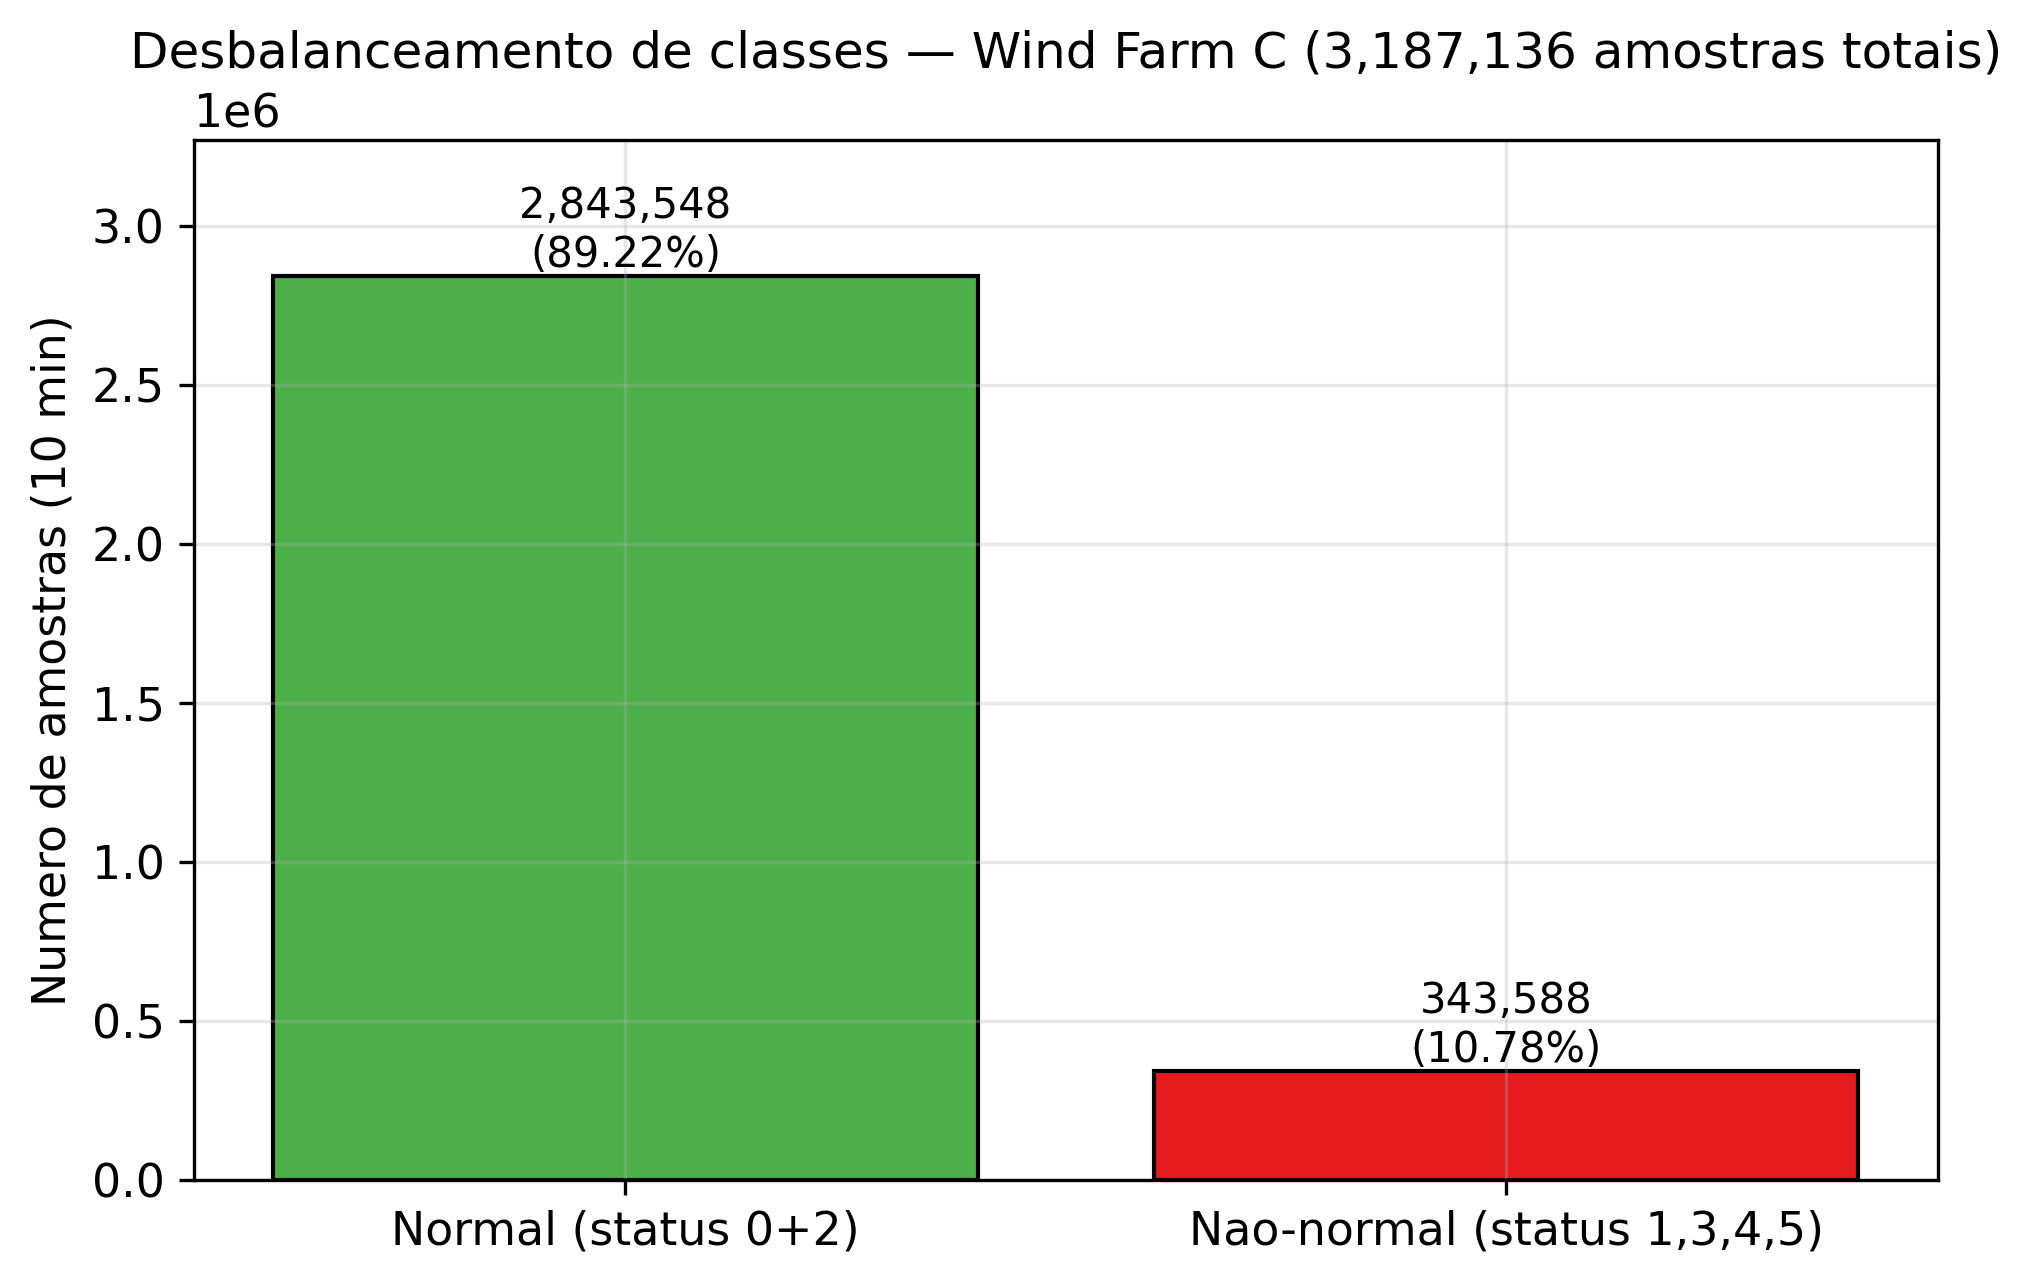
\includegraphics[width=0.75\textwidth]{figs/geradas/eda_desbalanceamento.png}
    \caption{Desbalanceamento de classes no Wind Farm C considerando \texttt{status\_type\_id}: estados \texttt{0} (Normal) $+$ \texttt{2} (Idling) vs.\ demais.}
    \label{fig:eda_desbalanceamento}
\end{figure}

A Figura~\ref{fig:eda_serie_potencia} ilustra a série temporal de potência gerada por uma turbina de exemplo (\texttt{power\_2\_avg}). A Figura~\ref{fig:eda_hist_vento} apresenta a distribuição de velocidade de vento (\texttt{wind\_speed\_236\_avg}). A Figura~\ref{fig:eda_correlacao} apresenta a matriz de correlação para um subconjunto de variáveis SCADA, evidenciando os blocos de redundância que motivam a etapa de seleção não supervisionada.

\begin{figure}[!ht]
    \centering
    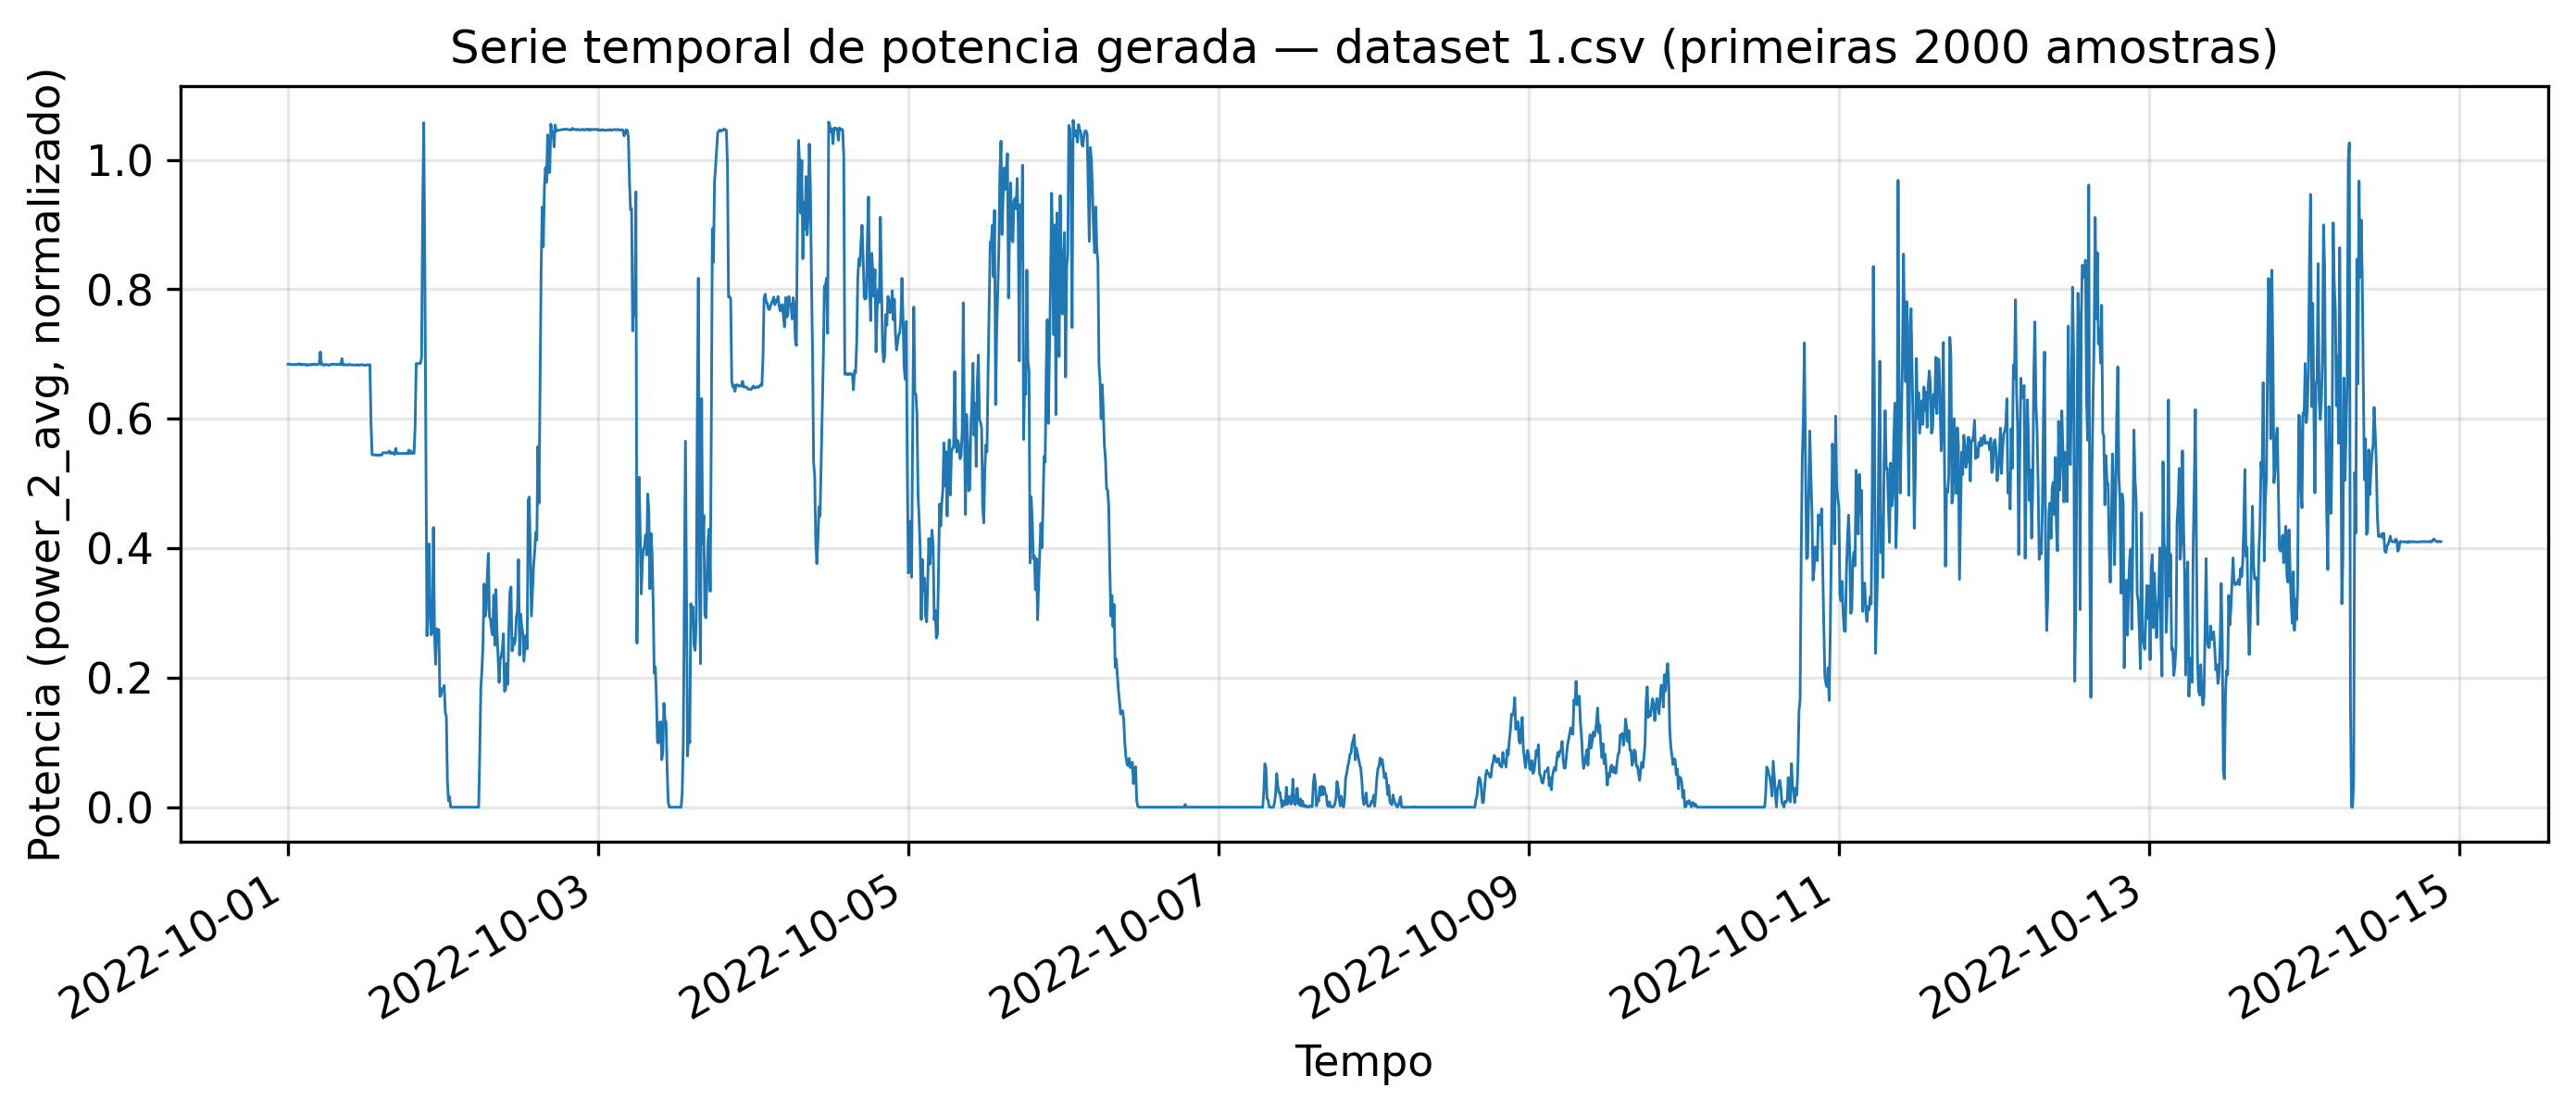
\includegraphics[width=0.95\textwidth]{figs/geradas/eda_serie_potencia.png}
    \caption{Série temporal de potência gerada (exemplo de turbina, primeiras 2000 amostras).}
    \label{fig:eda_serie_potencia}
\end{figure}

\begin{figure}[!ht]
    \centering
    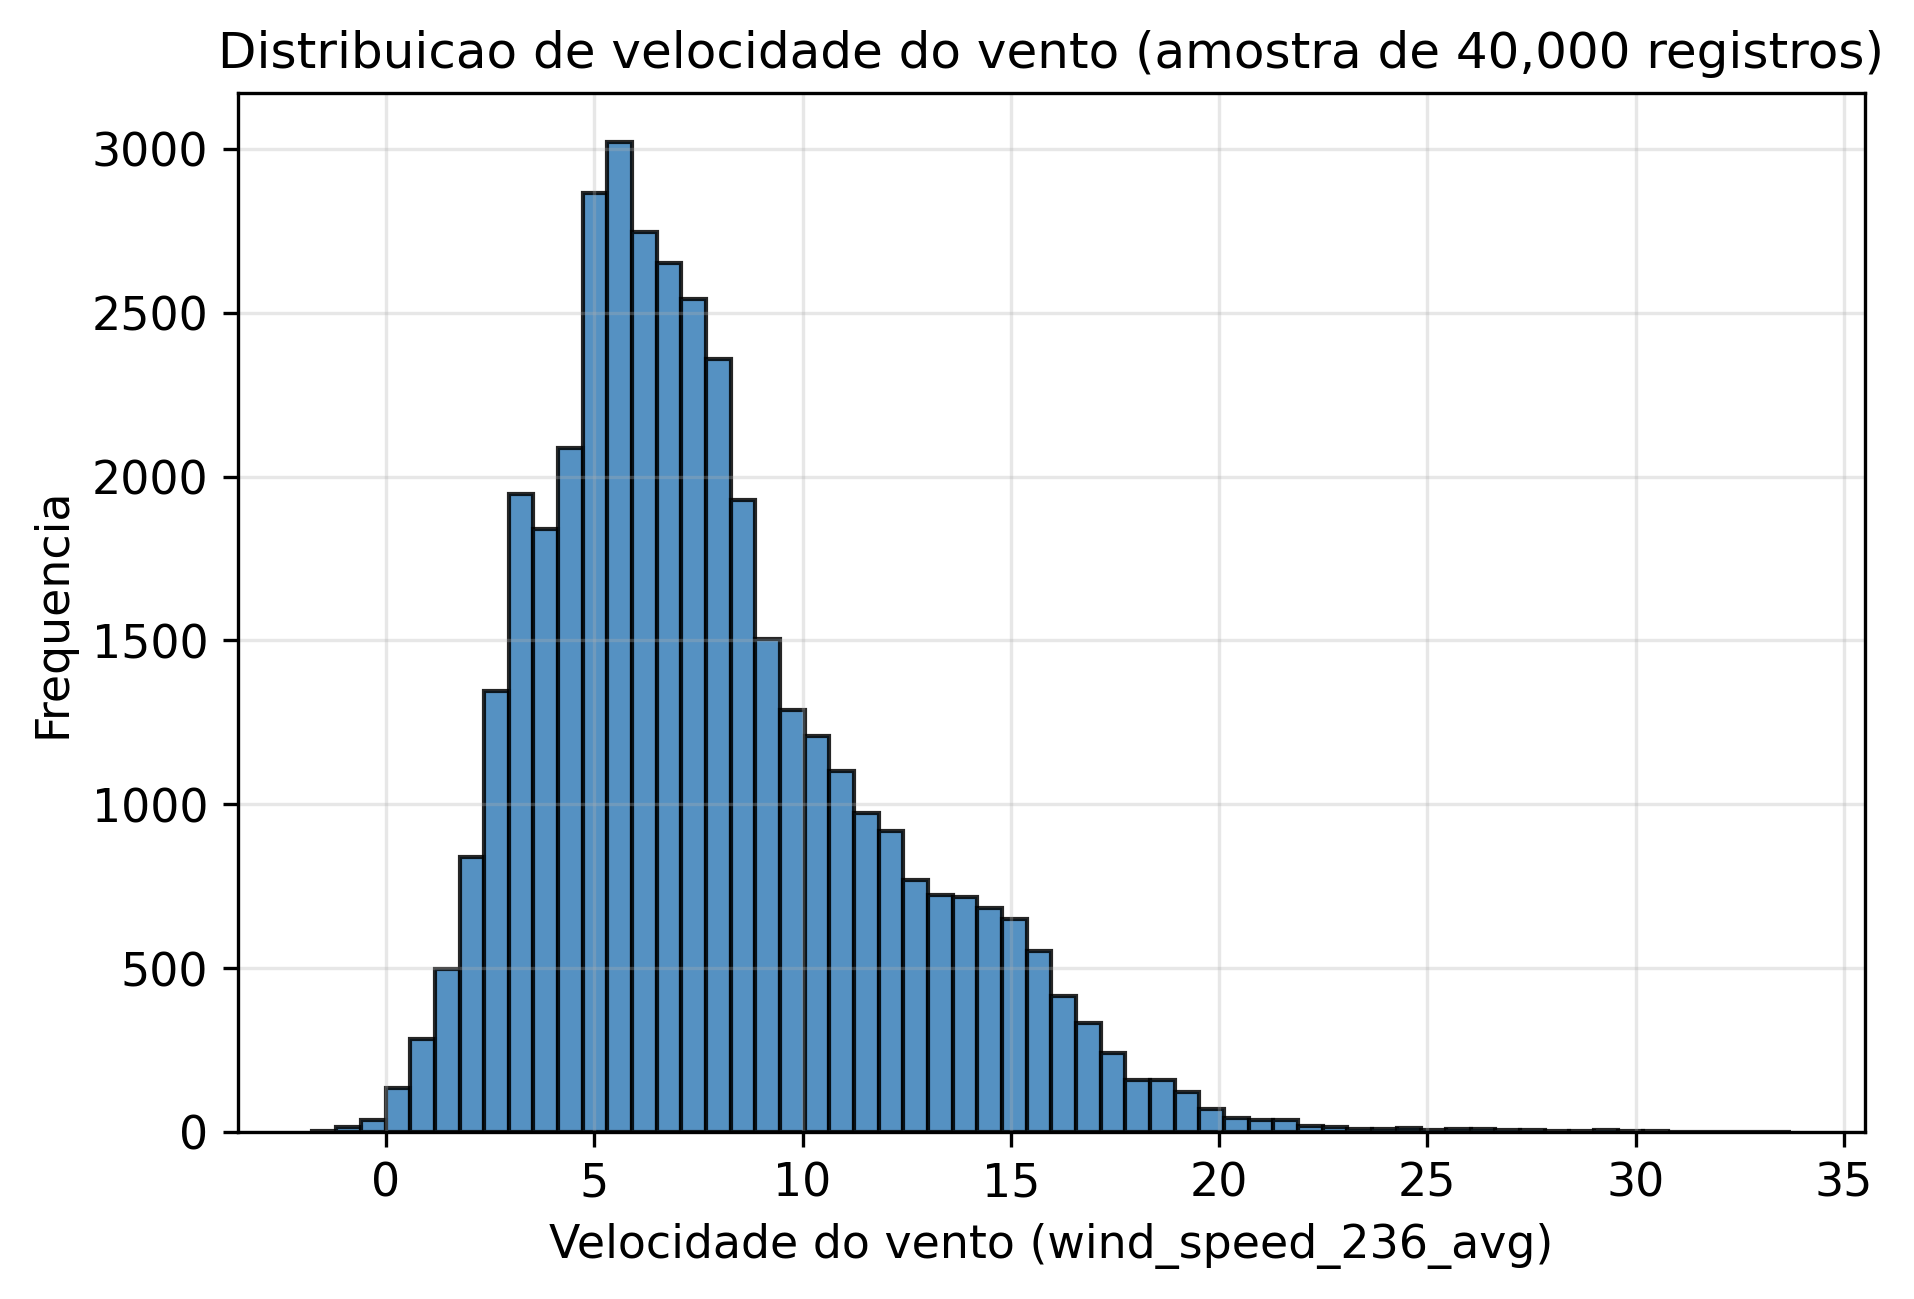
\includegraphics[width=0.7\textwidth]{figs/geradas/eda_hist_vento.png}
    \caption{Histograma de velocidade do vento (\texttt{wind\_speed\_236\_avg}, amostra de 40k registros).}
    \label{fig:eda_hist_vento}
\end{figure}

\begin{figure}[!ht]
    \centering
    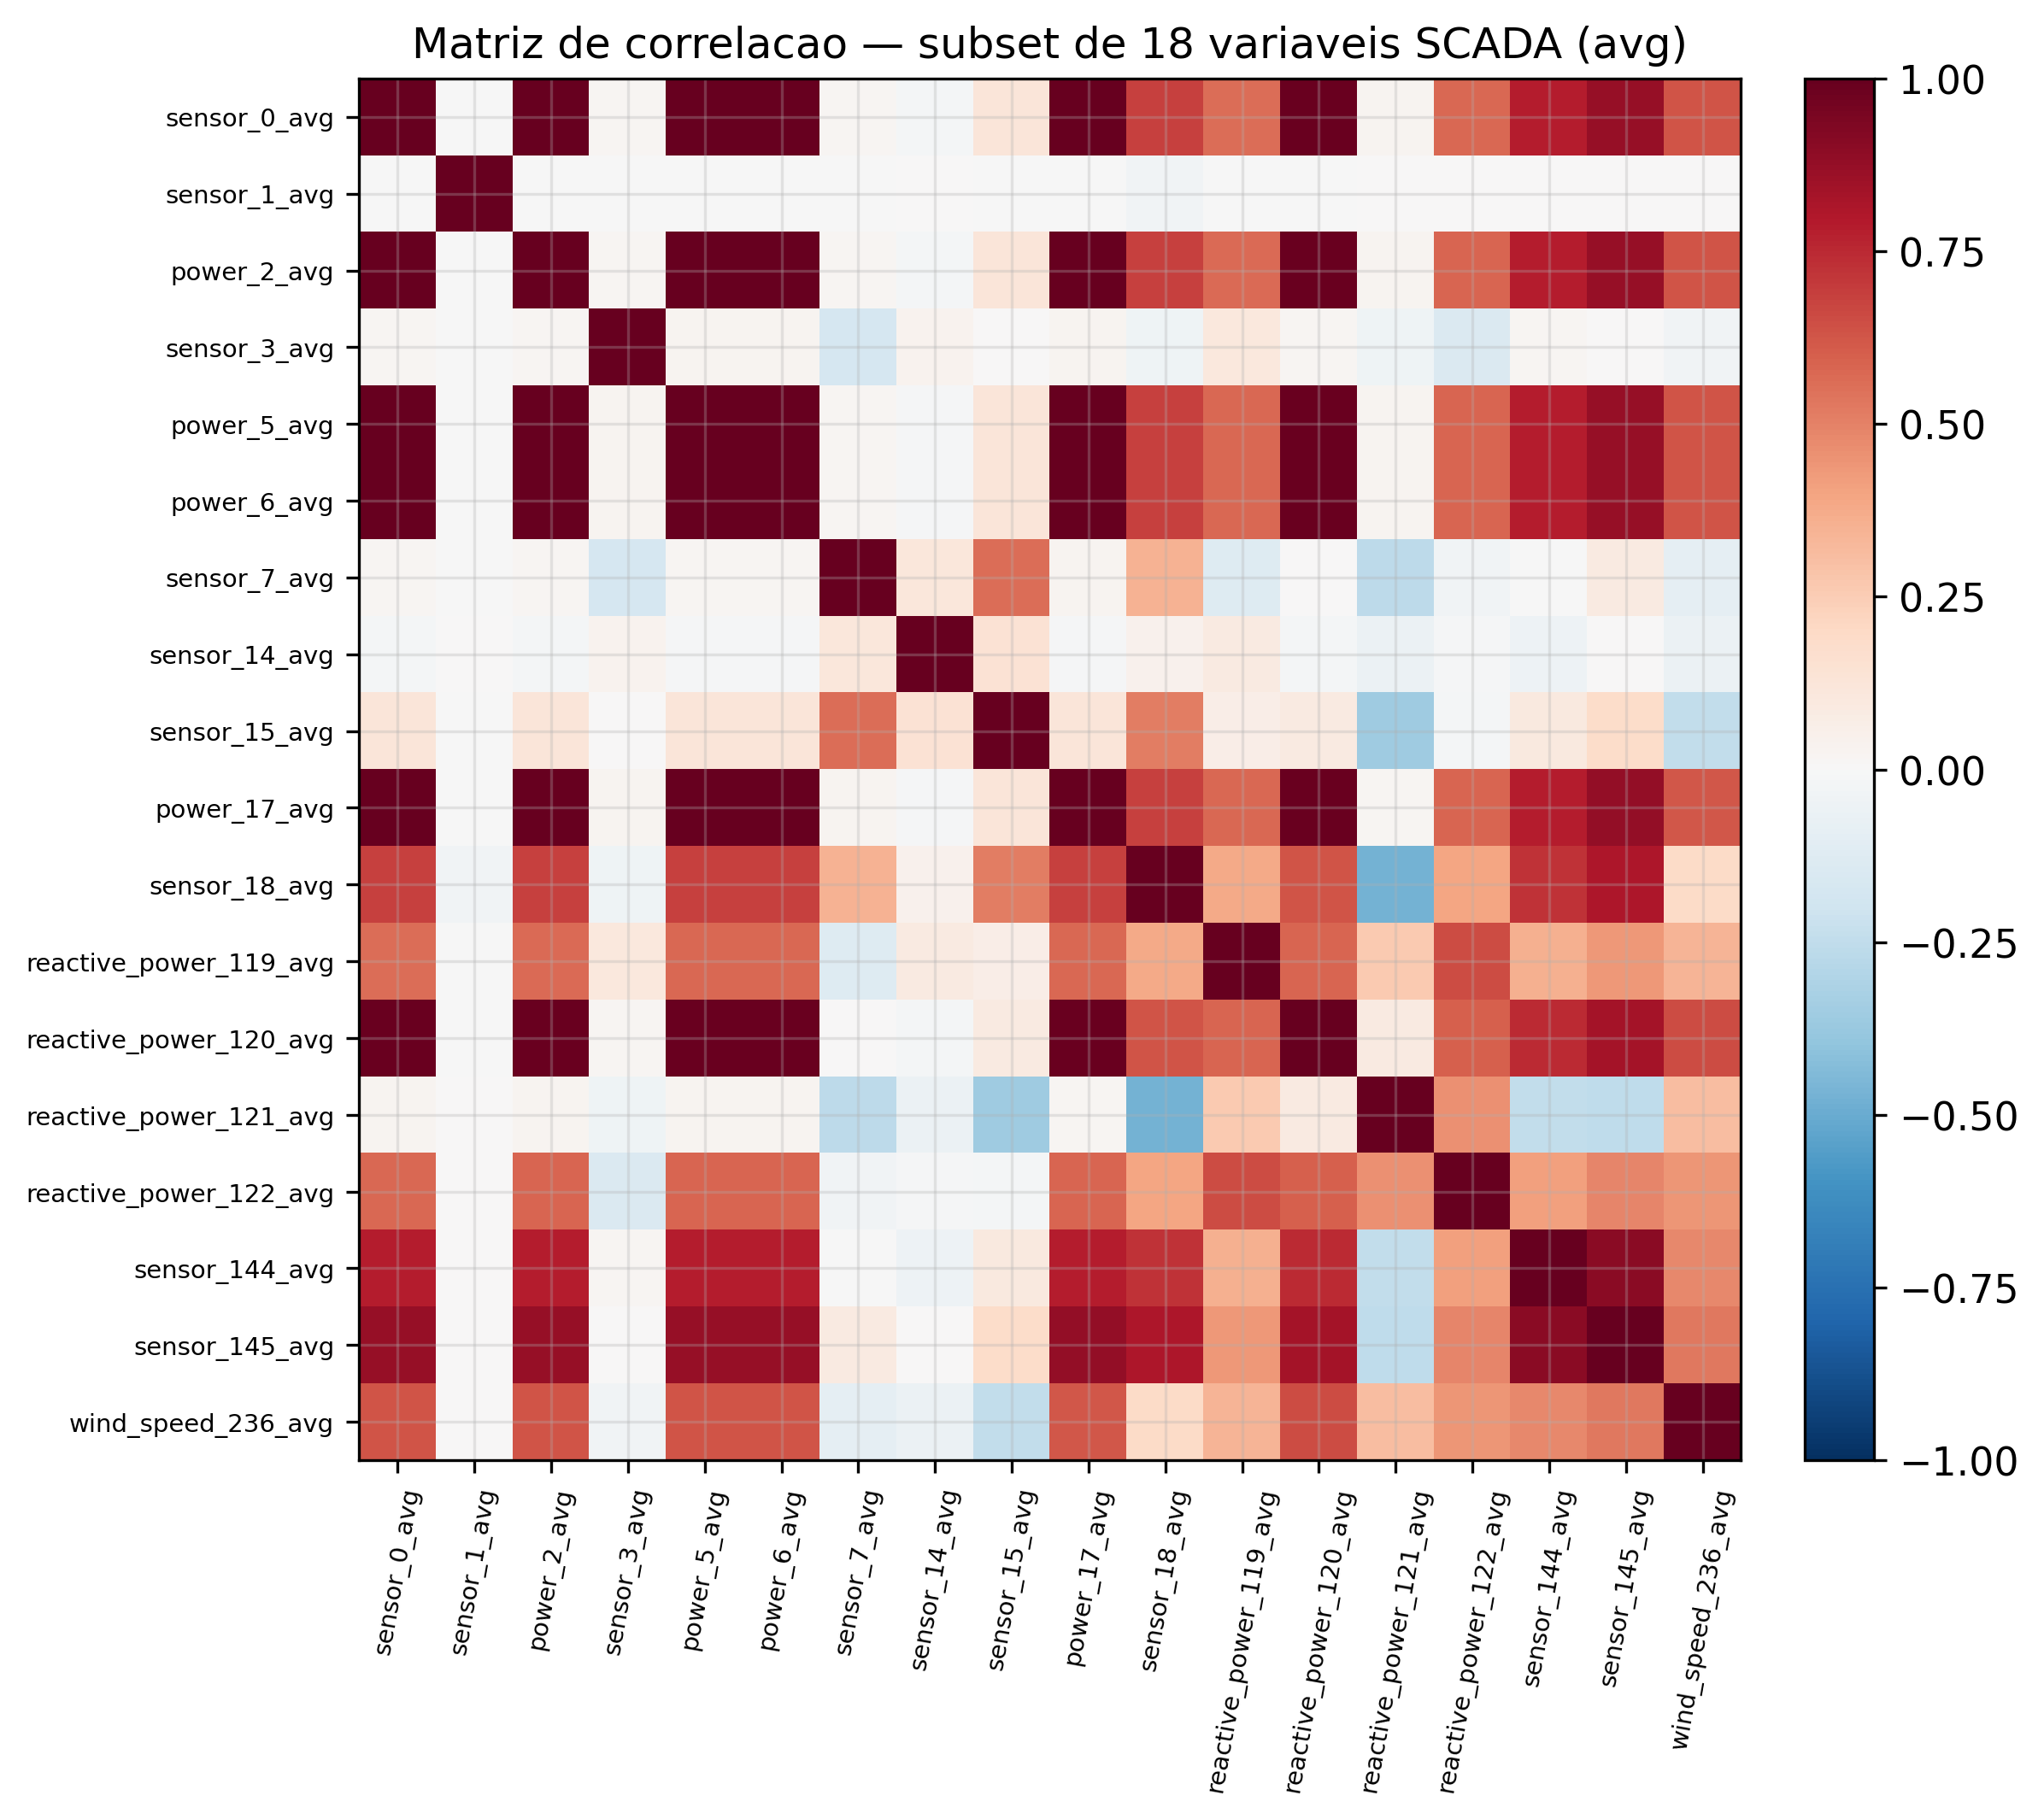
\includegraphics[width=0.85\textwidth]{figs/geradas/eda_matriz_correlacao.png}
    \caption{Matriz de correlação para subconjunto de variáveis SCADA (colunas \texttt{\_avg}).}
    \label{fig:eda_correlacao}
\end{figure}

\clearpage
\subsection{Modelos e Notebooks Implementados}

Cinco \textit{notebooks} foram implementados, divididos em dois paradigmas: supervisionado (NB1 e NB4) e não supervisionado (NB2, NB3 e NB5). A Tabela~\ref{tab:resumo_notebooks} apresenta uma visão geral; as subseções seguintes detalham cada implementação.

\begin{table}[!ht]
\centering
\small
\resizebox{\linewidth}{!}{%
\begin{tabular}{c|l|l|c|r}
\hline
\textbf{NB} & \textbf{Paradigma} & \textbf{Modelo} & \textbf{Framework} & \textbf{Parâmetros} \\
\hline
1 & Supervisionado         & CNN / LSTM / CNN-LSTM               & PyTorch        & $\sim$160\,K \\
2 & Não supervisionado     & CNN-BiLSTM-Attention Autoencoder    & PyTorch        & $\sim$954\,K \\
3 & Não supervisionado     & MLP Autoencoder + Optuna            & Keras/TF       & $\sim$150\,K \\
4 & Supervisionado + indução & MLP 3-classes + falhas sintéticas & Keras/TF       & $\sim$40\,K  \\
5 & Não supervisionado + indução & MLP Autoencoder + calibração induzida & Keras/TF & $\sim$40\,K \\
\hline
\end{tabular}%
}
\caption{Visão geral dos cinco notebooks implementados.}
\label{tab:resumo_notebooks}
\end{table}

\subsubsection{NB1 --- CNN-LSTM (Supervisionado, replicação Qi et al. 2024)}

Implementação em PyTorch baseada em \citet{Qi2024_CNN_LSTM_Energies}. Foram avaliadas três variantes: CNN pura, LSTM pura e CNN-LSTM híbrido ($\sim$160\,K parâmetros). A entrada é uma janela de 36 \textit{timesteps} (6 horas) $\times$ 285 \textit{features} (selecionadas via XGBoost \textit{scale\_pos\_weight}, top 30\% das 957 colunas (incluindo identificadores)). A saída é a classe binária \{Normal, Anomalia\}, com a regra ``\textit{any anomaly}'' (a janela é rotulada como anomalia se qualquer \textit{timestep} interno for anômalo). Loss CrossEntropy, otimizador Adam ($lr=10^{-3}$), \textit{batch} 600, até 500 épocas com \textit{early stopping} (\textit{patience}=20). Aplicou-se \textit{undersampling} 1:1 apenas no conjunto de treino (mantendo a distribuição natural $\sim$58:1 em validação e teste). O \textit{threshold} foi otimizado para maximizar $F_1$ na curva PR de validação.

\subsubsection{NB2 --- CNN-BiLSTM-Attention Autoencoder (Não supervisionado, PyTorch)}

Autoencoder profundo ($\sim$954\,K parâmetros) com \textit{encoder} composto por duas camadas Conv1D seguidas de duas camadas BiLSTM e uma camada \textit{MultiHeadAttention} de 4 cabeças (com conexão residual e LayerNorm). \textit{Decoder} LSTM simétrico. Entrada $36 \times 305$ \textit{features} (seleção não supervisionada por variância $+$ correlação). Loss MAE ($L_1$), otimizador Adam ($lr=10^{-4}$), \textit{batch} 64, até 100 épocas, \textit{early stopping} \textit{patience}=15, \textit{ReduceLROnPlateau} (\textit{factor}=0,5, \textit{patience}=3), AMP (\textit{Automatic Mixed Precision}) habilitado. Treinado \textbf{exclusivamente em janelas normais}. O \textit{score} de anomalia é o número de \textit{features} cujo erro de reconstrução excede o \textit{threshold} P95 (ou P99) calculado nas janelas normais da validação; se $\geq \mathtt{MIN\_FEATURES\_EXCEED}$ excederem (configurado dinamicamente como $5\%$ do número de \textit{features} efetivas, resultando em $15$ para 305 \textit{features}), a janela é classificada como anomalia. A versão v4 acrescenta cinco estratégias pós-hoc \textbf{sem re-treinar}: ponderação por AUROC, suavização temporal por voto majoritário, máscara informativa (\textit{features} com $\sigma_{\mathrm{erro}} > 0,01$), XGBoost pós-hoc sobre os erros, e \textit{threshold} Beta-$F_1$. \textbf{Importante:} a atenção é uma \textit{camada} dentro do encoder, não um Transformer completo.

\subsubsection{NB3 --- Dense MLP Autoencoder (Não supervisionado, Keras + Optuna)}

Autoencoder MLP simétrico em Keras/TensorFlow ($\sim$150\,K parâmetros), com \textit{encoder} 305$\to$200$\to$100$\to$35 (\textit{bottleneck}) e \textit{decoder} simétrico, ativações PReLU. \textbf{Sem janela temporal:} cada amostra de 10 minutos é processada independentemente como vetor de 305 \textit{features}. Loss MSE, otimizador Adam com \textit{ExponentialDecay} (\textit{lr} inicial $9{,}795 \times 10^{-4}$, \textit{decay\_rate} 0,9941), \textit{batch} 128, até 50 épocas, \textit{early stopping} \textit{patience}=5. Hiperparâmetros otimizados via Optuna em dois estudos sucessivos: \textbf{50 \textit{trials} para arquitetura} (\texttt{n\_layers} $\in [1,4]$, \texttt{code\_size} $\in [8,64]$, \texttt{learning\_rate} $\in [10^{-4}, 10^{-2}]$ em escala log, \texttt{decay\_rate} $\in [0{,}90, 0{,}999]$, $\gamma \in [0{,}01, 0{,}5]$) e \textbf{50 \textit{trials} para o $\gamma$ do \textit{threshold} adaptativo} (refinamento). O \textit{threshold} adaptativo segue $\tau_i = \widehat{\mathrm{RMSE}}(x_i) + \gamma$, onde $\widehat{\mathrm{RMSE}}$ é estimado por uma rede auxiliar. Avaliação no padrão CARE Score sobre os 58 eventos do Wind Farm C, com análise ARCANA para importância por \textit{feature} (implementadas inline no notebook --- ver Seção~\ref{sec:limitacoes}).

\subsubsection{NB4 --- Classifier MLP 3-class com Falhas Induzidas (Supervisionado)}

MLP de 3 classes (Normal / Anomalia Real / Anomalia Induzida) com \textit{data augmentation} via injeção de $7\%$ de falhas sintéticas no conjunto de treino. As perturbações são de três tipos: (i) ruído gaussiano com $3\sigma$ aplicado em blocos de 12 amostras; (ii) \textit{drift} com $5\sigma$ em metade do evento; (iii) \textit{spike} com $8\sigma$ em 1--5 pontos. Hiperparâmetros otimizados via Optuna (30 \textit{trials}): \texttt{n\_layers}=2, \texttt{hidden\_units}=192, \texttt{dropout}=0,29, \textit{lr}=$5{,}47 \times 10^{-3}$. Pré-processamento padrão: \texttt{DataClipper} $+$ \texttt{NanImputer} $+$ \texttt{StandardScaler}. \textit{Class\_weight} balanceado e \textit{threshold} otimizado por $F_1$ binário sobre PR de validação.

\subsubsection{NB5 --- Autoencoder MLP com Calibração por Falhas Induzidas (Não supervisionado)}

Autoencoder MLP treinado exclusivamente em dados normais (mesma família do NB3) e com \textit{threshold} calibrado via falhas sintéticas (mesma família do NB4). Três \textit{thresholds} são comparados: \textbf{Standard P95} (P95 sobre o RMSE das amostras normais de calibração), \textbf{Induced P95} (P95 sobre o RMSE das amostras normais $+$ injetadas, mais conservador) e \textbf{Adaptive} ($P50_{\mathrm{ind}} + \gamma$, onde $\gamma$ foi otimizado pelo Optuna em 30 \textit{trials} adicionais). Hiperparâmetros do AE: \texttt{n\_layers}=1, \texttt{code\_size}=57, \textit{lr}=$2{,}28 \times 10^{-3}$, \texttt{decay\_rate}=0,97, $\gamma$=0,749. A escolha final foi baseada no maior CARE Score entre as três opções.

\subsection{Data Processing}\label{subsec:tratamento_dados}

\subsubsection{Extração e Conversão}

Os 58 arquivos CSV do Wind Farm C (separador \texttt{;}) foram lidos com \texttt{pandas.read\_csv} e empilhados em um único \texttt{DataFrame} indexado pela coluna \texttt{time\_stamp}. As colunas de identificação (\texttt{asset\_id}, \texttt{id}, \texttt{train\_test}, \texttt{status\_type\_id}) são preservadas para servir de rótulo e estratificar os \textit{splits}; as 953 colunas restantes são as variáveis SCADA propriamente ditas, agrupadas por agregação (\texttt{*\_avg}, \texttt{*\_max}, \texttt{*\_min}, \texttt{*\_std}).

\subsubsection{Limpeza de Dados e Tratamento de Outliers}

A Figura~\ref{fig:eda_boxplot} mostra o efeito do \emph{clipping} aplicado por percentis (Q0,1\% e Q99,9\%) em variáveis representativas, etapa adotada pelo \texttt{DataClipper} dos notebooks NB2--NB5.

\begin{figure}[!ht]
    \centering
    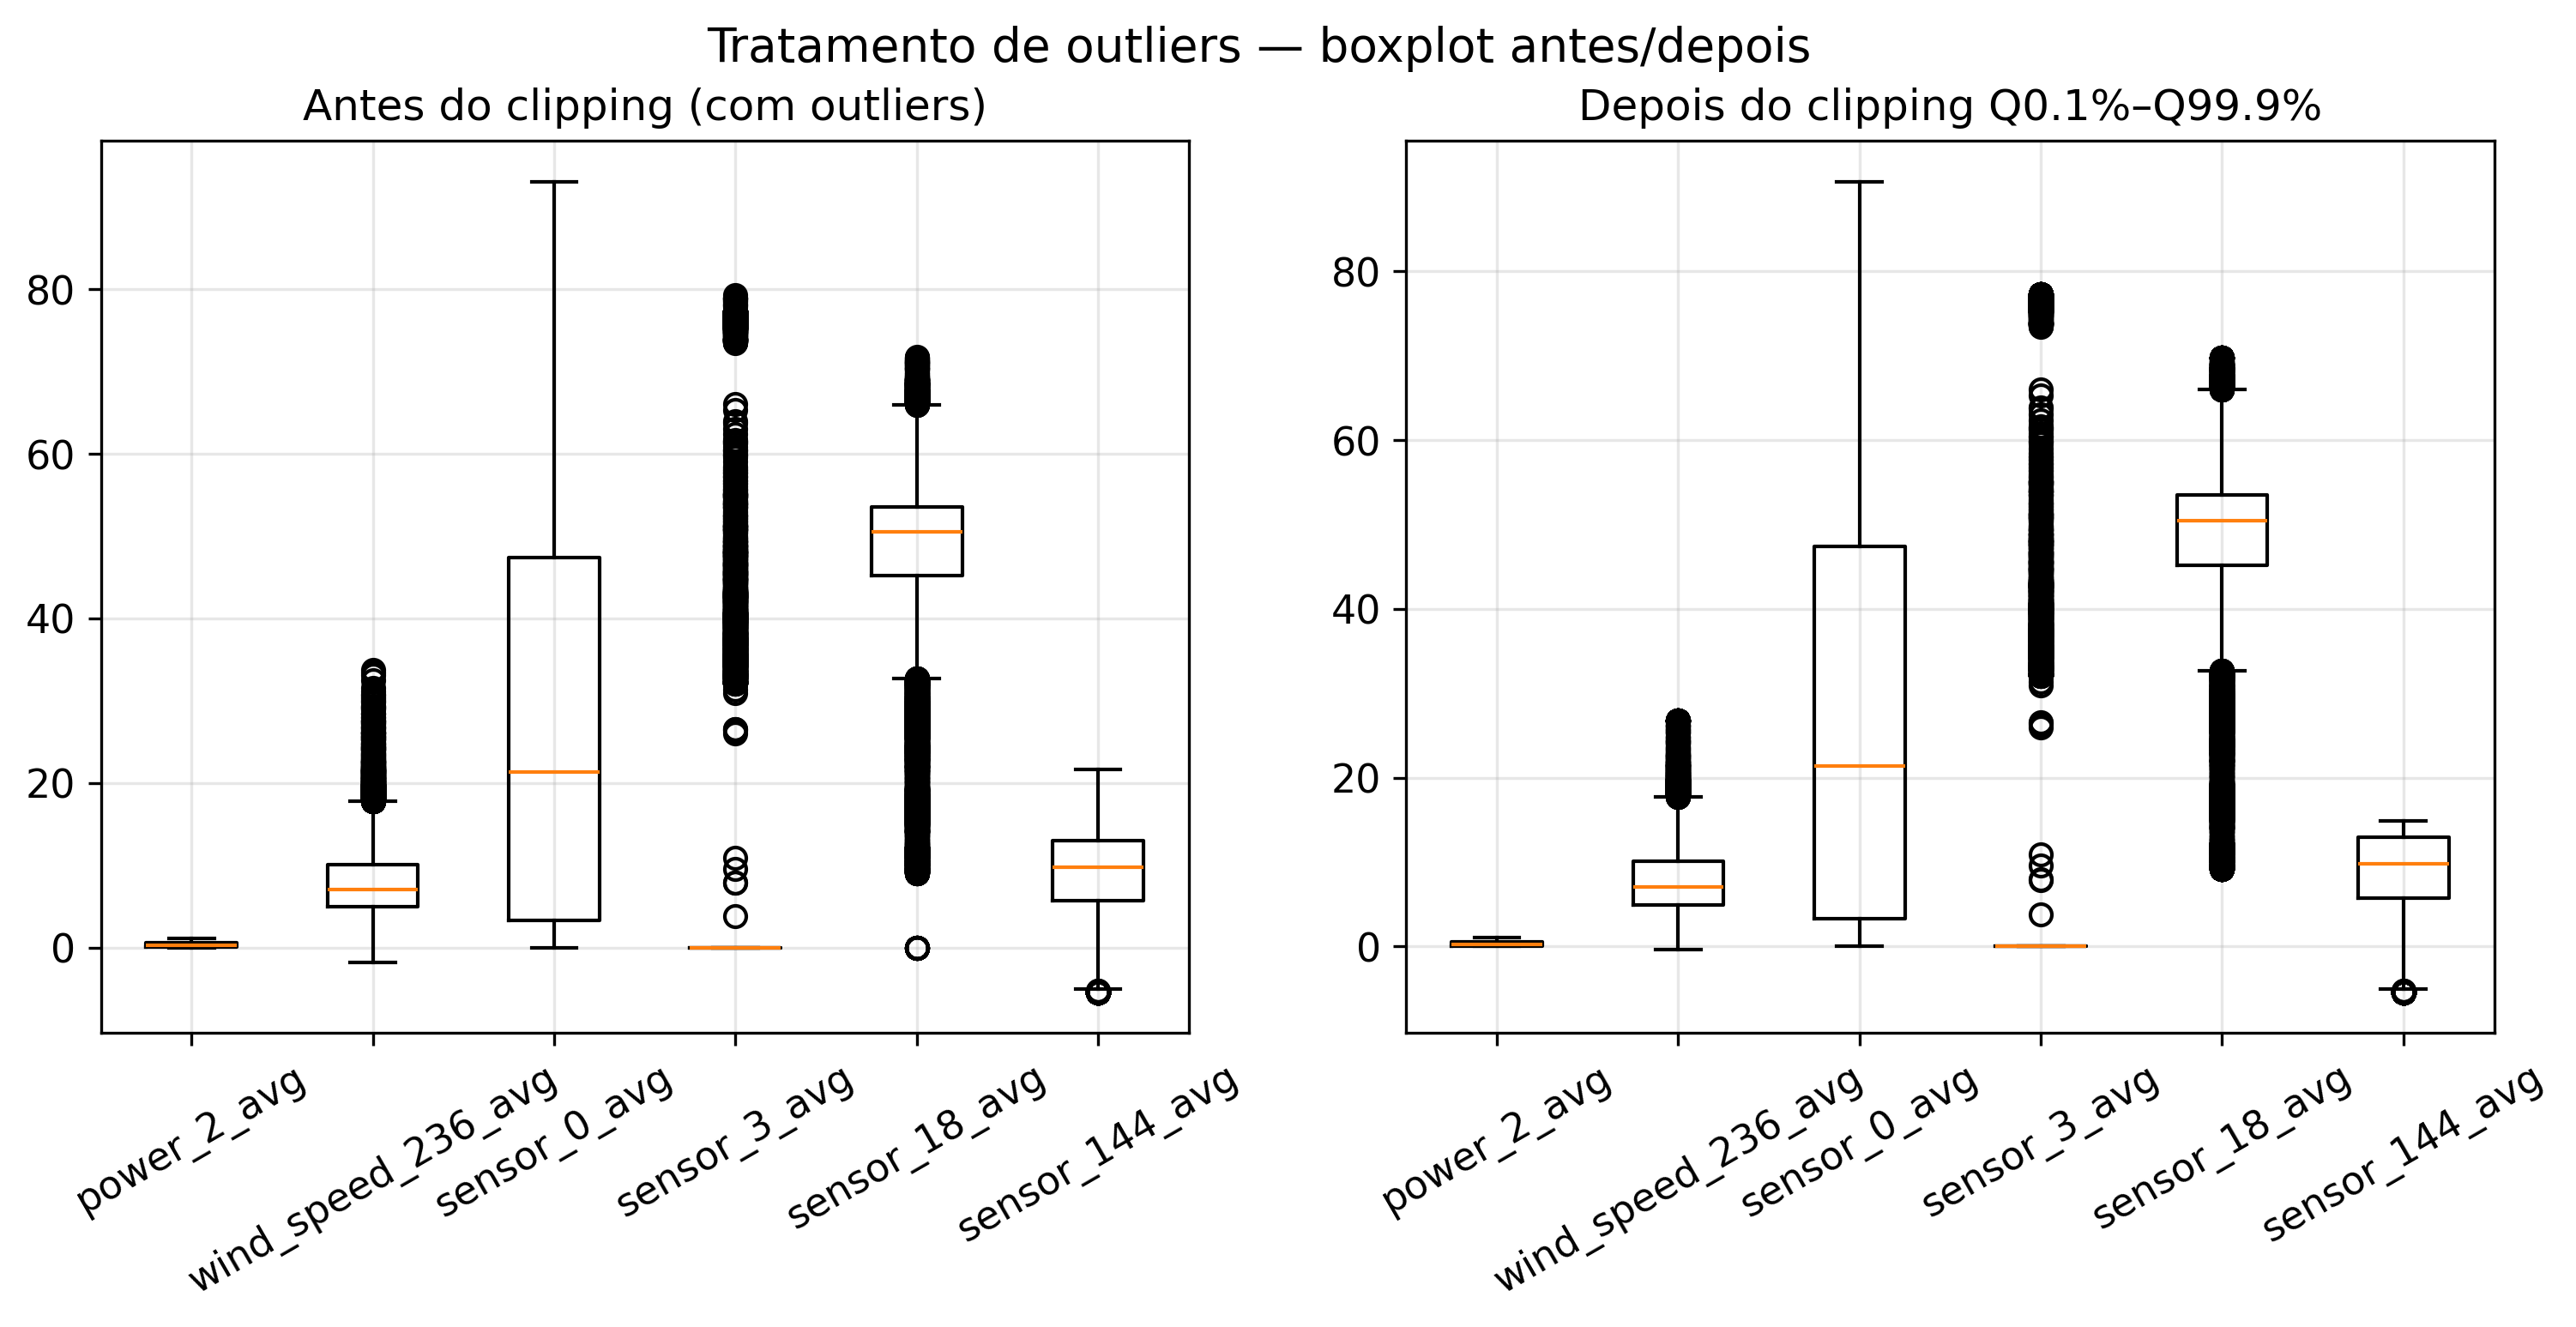
\includegraphics[width=0.95\textwidth]{figs/geradas/eda_boxplot_outliers.png}
    \caption{Boxplots antes e depois do \emph{clipping} Q0,1\%--Q99,9\% por feature.}
    \label{fig:eda_boxplot}
\end{figure}

\subsubsection{Imputação de Dados Faltantes}

Duas estratégias distintas de imputação foram empregadas. (i) \textbf{NB2:} cadeia temporal \texttt{ffill(limit=6)} $\rightarrow$ \texttt{bfill(limit=6)} $\rightarrow$ \texttt{fillna(0)}, aplicada por evento, preservando continuidade temporal e limitando a propagação a no máximo uma hora (6 amostras de 10 minutos) em cada direção. (ii) \textbf{NB3, NB4 e NB5:} \texttt{NanImputer} sklearn-compatível (módulo \texttt{induced\_failure\_utils.py}) que preenche valores faltantes com a \textbf{média da coluna} computada apenas sobre o conjunto de treino normal --- escolha consistente com o uso posterior de \texttt{StandardScaler} no mesmo \textit{pipeline}.

\subsubsection{Sincronização Temporal}

Como todos os sensores SCADA do CARE\_To\_Compare são amostrados de forma síncrona em janelas de 10 minutos, não foi necessário interpolar para uma resolução comum. A sincronização restringe-se à garantia de que o índice temporal seja monotonicamente crescente e à remoção de duplicatas eventuais antes da construção das janelas deslizantes.

\subsubsection{Seleção de Variáveis (Feature Selection)}

\begin{sloppypar}
Duas estratégias foram comparadas. (i) \textbf{Supervisionada (NB1):} XGBoost com \texttt{scale\_pos\_weight} ajustado ao desbalanceamento, treinado sobre amostra de 100\,K linhas, com seleção das 30\% \textit{features} mais importantes por \textit{gain} (resultado: 285 \textit{features}). (ii) \textbf{Não supervisionada (NB2--NB5):} pipeline de três filtros encadeados --- remoção de variância $< 10^{-4}$, remoção de \textit{features} com correlação $< 0{,}1$ com as variáveis operacionais (potência, velocidade do vento, sensores 144 e 145 e variantes), e remoção de \textit{features} com correlação $> 0{,}95$ entre si (resultado: 305 \textit{features}). A versão supervisionada captura discriminabilidade direta mas exige rótulos; a não supervisionada é mais robusta a cenários novos.
\end{sloppypar}

\subsubsection{Normalização e Escalonamento}

Dois escalonadores foram adotados conforme o paradigma do modelo. (i) \textbf{NB1 e NB2:} \texttt{MinMaxScaler} para o intervalo $[0,1]$, adequado às ativações SELU/Sigmoid utilizadas. (ii) \textbf{NB3, NB4 e NB5:} \texttt{StandardScaler} (z-score, $\mu=0$, $\sigma=1$), padrão para arquiteturas Keras/TensorFlow com \texttt{PReLU} e otimizadores baseados em gradiente. Em \textbf{todos os casos}, o escalonador é ajustado \textbf{somente nos dados normais do treino} para evitar \textit{data leakage}, e a mesma transformação é aplicada à validação e ao teste. Para variáveis angulares (graus), foi feita expansão em pares \textit{sin}/\textit{cos}, preservando a continuidade circular (e.g., 359° e 1° passam a ser próximos no espaço transformado).

\subsection{Hiperparâmetros e Otimização}

A Tabela~\ref{tab:hp_resumo} resume os hiperparâmetros finais por \textit{notebook}.

\begin{table}[!ht]
\centering
\small
\resizebox{\linewidth}{!}{%
\begin{tabular}{l|l|l|l|l|l}
\hline
\textbf{Notebook} & \textbf{Loss} & \textbf{Otimizador / lr} & \textbf{Batch} & \textbf{Épocas} & \textbf{Early Stop} \\
\hline
NB1 (CNN/LSTM/CNN-LSTM) & CrossEntropy & Adam / $10^{-3}$ & 600 & 500 & p=20 \\
NB2 (CNN-BiLSTM-Att AE) & MAE          & Adam / $10^{-4}$ & 64  & 100 & p=15 \\
NB3 (Keras MLP AE)      & MSE          & Adam ExpDecay / $9{,}8\!\times\!10^{-4}$ & 128 & 50  & p=5  \\
NB4 (Classifier 3-cls)  & CrossEntropy & Adam / $5{,}5\!\times\!10^{-3}$ & 128 & 100 & p=10 \\
NB5 (AE Induced Calib)  & MSE          & Adam Decay / $2{,}3\!\times\!10^{-3}$ & 128 & 200 & p=10 \\
\hline
\end{tabular}%
}
\caption{Hiperparâmetros finais por notebook.}
\label{tab:hp_resumo}
\end{table}

NB3, NB4 e NB5 utilizaram \textbf{Optuna} para busca automatizada de hiperparâmetros (50+50, 30 e 30+30 \textit{trials}, respectivamente --- nos casos com soma, o primeiro número refere-se à arquitetura do AE e o segundo ao $\gamma$ do \textit{threshold}). Os demais foram ajustados manualmente seguindo a configuração do paper original (NB1) ou por inspeção iterativa de curvas de loss (NB2).

\subsection{Estratégia de Validação}\label{subsec:validacao}

\begin{sloppypar}
Três estratégias de \textit{split} foram empregadas, refletindo a natureza de cada paradigma e a forma do dataset. (i) \textbf{NB1 e NB4 --- divisão por evento:} 40 treino / 8 validação / 10 teste no NB1; 70/15/15 sobre o conjunto de \texttt{event\_id}s no NB4 com \textit{seed} fixo, evitando \textit{leakage} entre janelas que compartilhem o mesmo evento de falha. (ii) \textbf{NB2 --- divisão temporal 70/15/15:} pontos de corte calculados \emph{dinamicamente} a partir do percentil 70 e 85 dos \texttt{time\_stamp}s agregados de todos os 58 datasets, agrupando todos os eventos no mesmo eixo temporal. (iii) \textbf{NB3 e NB5 --- coluna \texttt{train\_test} do CARE:} aproveitam o particionamento sugerido pelo próprio dataset (\texttt{train} vs.\ \texttt{prediction}, equivalente a teste), com sub-divisão temporal interna 80/20 do treino para calibração. Em todos os casos, o escalonador é ajustado apenas nos dados normais do treino, e \textit{thresholds} são calibrados sobre a validação.
\end{sloppypar}

\subsection{Reprodutibilidade}

\begin{sloppypar}
Sementes aleatórias fixadas em 42 para todos os geradores (\texttt{numpy}, \texttt{torch}, \texttt{tensorflow}, \texttt{random}). Versões principais: Python 3.10, PyTorch 2.x com CUDA 12.x, TensorFlow/Keras 2.x, scikit-learn 1.5+, Optuna 3.x, XGBoost 2.x. O ambiente está fixado em \texttt{notebooks/requirements.txt}. Todos os \textit{notebooks} possuem suas versões \texttt{.py} sincronizadas em \texttt{notebooks/} para execução em modo \textit{script}.
\end{sloppypar}

% ─── 6 EXPERIMENTOS ──────────────────────────────────────────────────────────
\section{Experimentos}

\subsection{Configuração Experimental}

O dataset \emph{CARE\_To\_Compare} Wind Farm C contém aproximadamente 3,18 milhões de amostras de SCADA com 957 colunas (incluindo identificadores), totalizando dezenas de gigabytes em memória após o \emph{stack} de janelas deslizantes. Devido a esse volume, os treinamentos têm custo computacional elevado e \textbf{exigem hardware especializado para operações matriciais}, como GPUs ou TPUs --- a execução em CPU é inviável tanto pelo tempo (estimativas indicam ordem de dias por experimento de \emph{deep learning}) quanto pela memória requerida pelas multiplicações tensoriais densas dos modelos CNN, BiLSTM, Atenção e MLP. Os experimentos foram conduzidos em estações com GPU NVIDIA RTX 4060 (8\,GB) para prototipagem e em \emph{workstation} com NVIDIA RTX A6000 (48\,GB) para treinamentos finais, com uso de \emph{mixed precision} (AMP) no NB2 para caber em memória. Sem GPU dedicada, a reprodução completa do pipeline (Optuna com 100 \emph{trials}, treinamento dos cinco notebooks e cálculo do CARE Score por evento) seria impraticável.

\subsection{Experimentos sem Dados Exógenos}

Esta foi a configuração efetivamente executada em todos os cinco \textit{notebooks}: os modelos consomem apenas as variáveis SCADA do Wind Farm C, sem qualquer enriquecimento meteorológico. Os resultados destes experimentos constituem o corpo central da Seção~\ref{sec:resultados-obtidos} e são utilizados na comparação entre os paradigmas supervisionado e não supervisionado.

\subsection{Experimentos com Dados Exógenos}

\begin{sloppypar}
Esta classe de experimentos era prevista pelo plano original (variante ``com'' vs.\ ``sem'' dados meteorológicos), mas \textbf{não foi executada} porque a anonimização do dataset CARE\_To\_Compare suprime as coordenadas geográficas e datas absolutas dos parques eólicos, inviabilizando o alinhamento espaço-temporal com bases meteorológicas externas (CPTEC/INPE, OpenWeatherMap). Detalhes da inviabilidade técnica são discutidos na Seção~\ref{sec:problemas-dados}. Como consequência, a comparação direta ``com vs.\ sem dados exógenos'' foi substituída pela comparação entre paradigmas (supervisionado vs.\ não supervisionado) e pela exploração de \textit{data augmentation} via falhas sintéticas (NB4 e NB5).
\end{sloppypar}

\subsection{Ablation Study}

O NB2 v4 funcionou efetivamente como um estudo de ablação \textbf{pós-treino}: a partir do mesmo modelo CNN-BiLSTM-Attention treinado, foram avaliadas cinco estratégias incrementais sobre o \textit{score} de anomalia. A Tabela~\ref{tab:ablation_nb2} consolida o impacto de cada componente.

\begin{table}[!ht]
\centering
\small
\begin{tabular}{l|c|c|c|c}
\hline
\textbf{Configuração} & \textbf{Precision} & \textbf{Recall} & $\boldsymbol{F_1}$ & \textbf{AUC-ROC} \\
\hline
v3 P95 (baseline)               & 0,016 & \textbf{0,965} & 0,032 & 0,864 \\
v3 P99                          & 0,030 & 0,885 & \textbf{0,058} & 0,864 \\
v4 Score Pond.\ + Beta-$F_1$    & 0,023 & 0,883 & 0,045 & \textbf{0,872} \\
v4 Suavização $K=5$             & 0,023 & 0,883 & 0,045 & --- \\
v4 P95 + Máscara informativa    & 0,016 & 0,946 & 0,032 & 0,864 \\
v4 XGBoost pós-hoc              & 0,000 & 0,000 & 0,000 & 0,743 \\
\hline
\end{tabular}
\caption{Ablação pós-treino do NB2: impacto de cada estratégia v4.}
\label{tab:ablation_nb2}
\end{table}

A ponderação por AUROC e o \textit{threshold} Beta-$F_1$ produziram a maior AUC-ROC (0,872), mas o XGBoost pós-hoc colapsou no teste (\textit{precision}=\textit{recall}=0) apesar de AUC=0,743 --- o \textit{threshold} aprendido na validação não generalizou. No NB5, a ablação se manifesta na comparação entre os três \textit{thresholds} (Standard P95, Induced P95, Adaptive), conforme Figura~\ref{fig:nb5_tradeoff}.

\subsection{Custo Computacional}

A Tabela~\ref{tab:custo_comp} resume o custo computacional estimado por \textit{notebook}, medido nos equipamentos descritos na Seção~6.1 (RTX 4060 para prototipagem e RTX A6000 para treinamento final). Os valores de tempo referem-se ao treinamento completo incluindo a busca por hiperparâmetros via Optuna quando aplicável; os \textit{notebooks} sem Optuna (NB1 e NB2) foram ajustados manualmente.

\begin{table}[!ht]
\centering
\small
\resizebox{\linewidth}{!}{%
\begin{tabular}{c|r|r|l|l}
\hline
\textbf{NB} & \textbf{Parâmetros} & \textbf{\textit{Trials} Optuna} & \textbf{Tempo aprox.\ (GPU A6000)} & \textbf{Memória GPU} \\
\hline
1 & $\sim$160\,K  & ---  & $\sim$1--2\,h (500 épocas, batch 600)         & $<$2\,GB \\
2 & $\sim$954\,K  & ---  & $\sim$3--5\,h (100 épocas, AMP, batch 64)     & $\sim$6--8\,GB \\
3 & $\sim$150\,K  & 50+50 & $\sim$4--8\,h (50 épocas $\times$ 100 \textit{trials}) & $<$2\,GB \\
4 & $\sim$40\,K   & 30   & $\sim$1--2\,h (100 épocas $\times$ 30 \textit{trials})  & $<$1\,GB \\
5 & $\sim$40\,K   & 30+30 & $\sim$2--3\,h (200 épocas $\times$ 60 \textit{trials}) & $<$1\,GB \\
\hline
\end{tabular}%
}
\caption{Custo computacional estimado por \textit{notebook} (GPU NVIDIA RTX A6000, 48\,GB).}
\label{tab:custo_comp}
\end{table}

O NB2 é o mais custoso em memória por combinar janelas $36 \times 305$, BiLSTM bidirecional e \textit{MultiHeadAttention}; o uso de AMP (\textit{Automatic Mixed Precision}) foi necessário para caber em 8\,GB na RTX 4060. O NB3 é o mais custoso em tempo de \textit{wall-clock} por somar os 100 \textit{trials} Optuna para arquitetura e para o $\gamma$ do \textit{threshold} adaptativo. Inferência (cálculo do \textit{score} de anomalia sobre o conjunto de teste) é negligenciável em todos os casos ($<$30\,s).

% ─── 7 PROBLEMAS COM DADOS ───────────────────────────────────────────────────
\section{Problemas com Dados}\label{sec:problemas-dados}

\subsection{Escassez de Dados de Anomalia}

O Wind Farm C contém aproximadamente 3,18 milhões de amostras de 10 minutos, das quais somente $\sim$1,9\% pertencem a períodos rotulados como anomalia em nível de \textit{event\_label} (razão Normal:Anomalia $\approx$ 51:1). Em nível de \texttt{status\_type\_id} (Figura~\ref{fig:eda_desbalanceamento}), o desbalanceamento se reduz para 89:11 porque ali são contabilizados também estados de manutenção e alarmes operacionais. Em qualquer das duas visões, métricas como acurácia tornam-se enganosas (um classificador trivial que sempre prevê ``Normal'' atinge 89--98\% de acurácia sem detectar nenhuma falha), justificando o uso prioritário de $F_1$, AUC-ROC e CARE Score.

\subsection{Localização Não Divulgada dos Sítios}

Os repositórios públicos de dados SCADA, incluindo o CARE\_To\_Compare, anonimizam completamente a localização geográfica dos parques eólicos (apenas identificadores genéricos como Wind Farm A, B, C) e substituem datas absolutas por datas deslocadas. Essa prática é motivada por restrições contratuais e de confidencialidade comercial: a posição exata permitiria identificar o operador e correlacionar dados sensíveis de produção com eventos públicos.

\subsection{Impossibilidade de Uso de Dados Meteorológicos Externos}

O dataset CARE\_To\_Compare anonimiza completamente a localização das turbinas: os três parques são identificados apenas como Wind Farm A, B e C, sem coordenadas geográficas (latitude/longitude), e os \textit{timestamps} são deslocados por um offset desconhecido, eliminando as datas absolutas reais. Essas duas peças de informação são pré-requisito indispensável para alinhar espacialmente e temporalmente os dados SCADA com bases meteorológicas externas como o CPTEC/INPE ou a API do OpenWeatherMap: sem as coordenadas, não é possível selecionar a estação meteorológica mais próxima; sem as datas absolutas, não é possível indexar os registros climáticos na janela temporal correta.

Como consequência direta, a comparação central prevista no plano FAPESP --- ``modelos com vs.\ sem dados exógenos'' --- não pôde ser executada. O projeto foi readequado para focar na comparação entre paradigmas de detecção (supervisionado vs.\ não supervisionado) e na exploração de técnicas alternativas para lidar com a escassez de amostras anômalas: \textit{data augmentation} via injeção de falhas sintéticas (NB4 e NB5). Essa limitação é recorrente em pesquisa com dados SCADA públicos e raramente discutida explicitamente na literatura, o que reforça a importância de documentá-la aqui.

\subsection{Qualidade dos Dados SCADA}

A Figura~\ref{fig:eda_missing} apresenta um mapa de calor da fração de valores faltantes ou zero (proxy de sensor inativo) por dataset $\times$ feature, em uma amostra dos arquivos. Áreas claras indicam blocos com instrumentação inativa ou sensores fora de operação naquele período --- justificando as etapas de imputação descritas na Seção~\ref{subsec:tratamento_dados} (\texttt{ffill}/\texttt{bfill}/zeros no NB2; média da coluna nos NB3--NB5).

\begin{figure}[!ht]
    \centering
    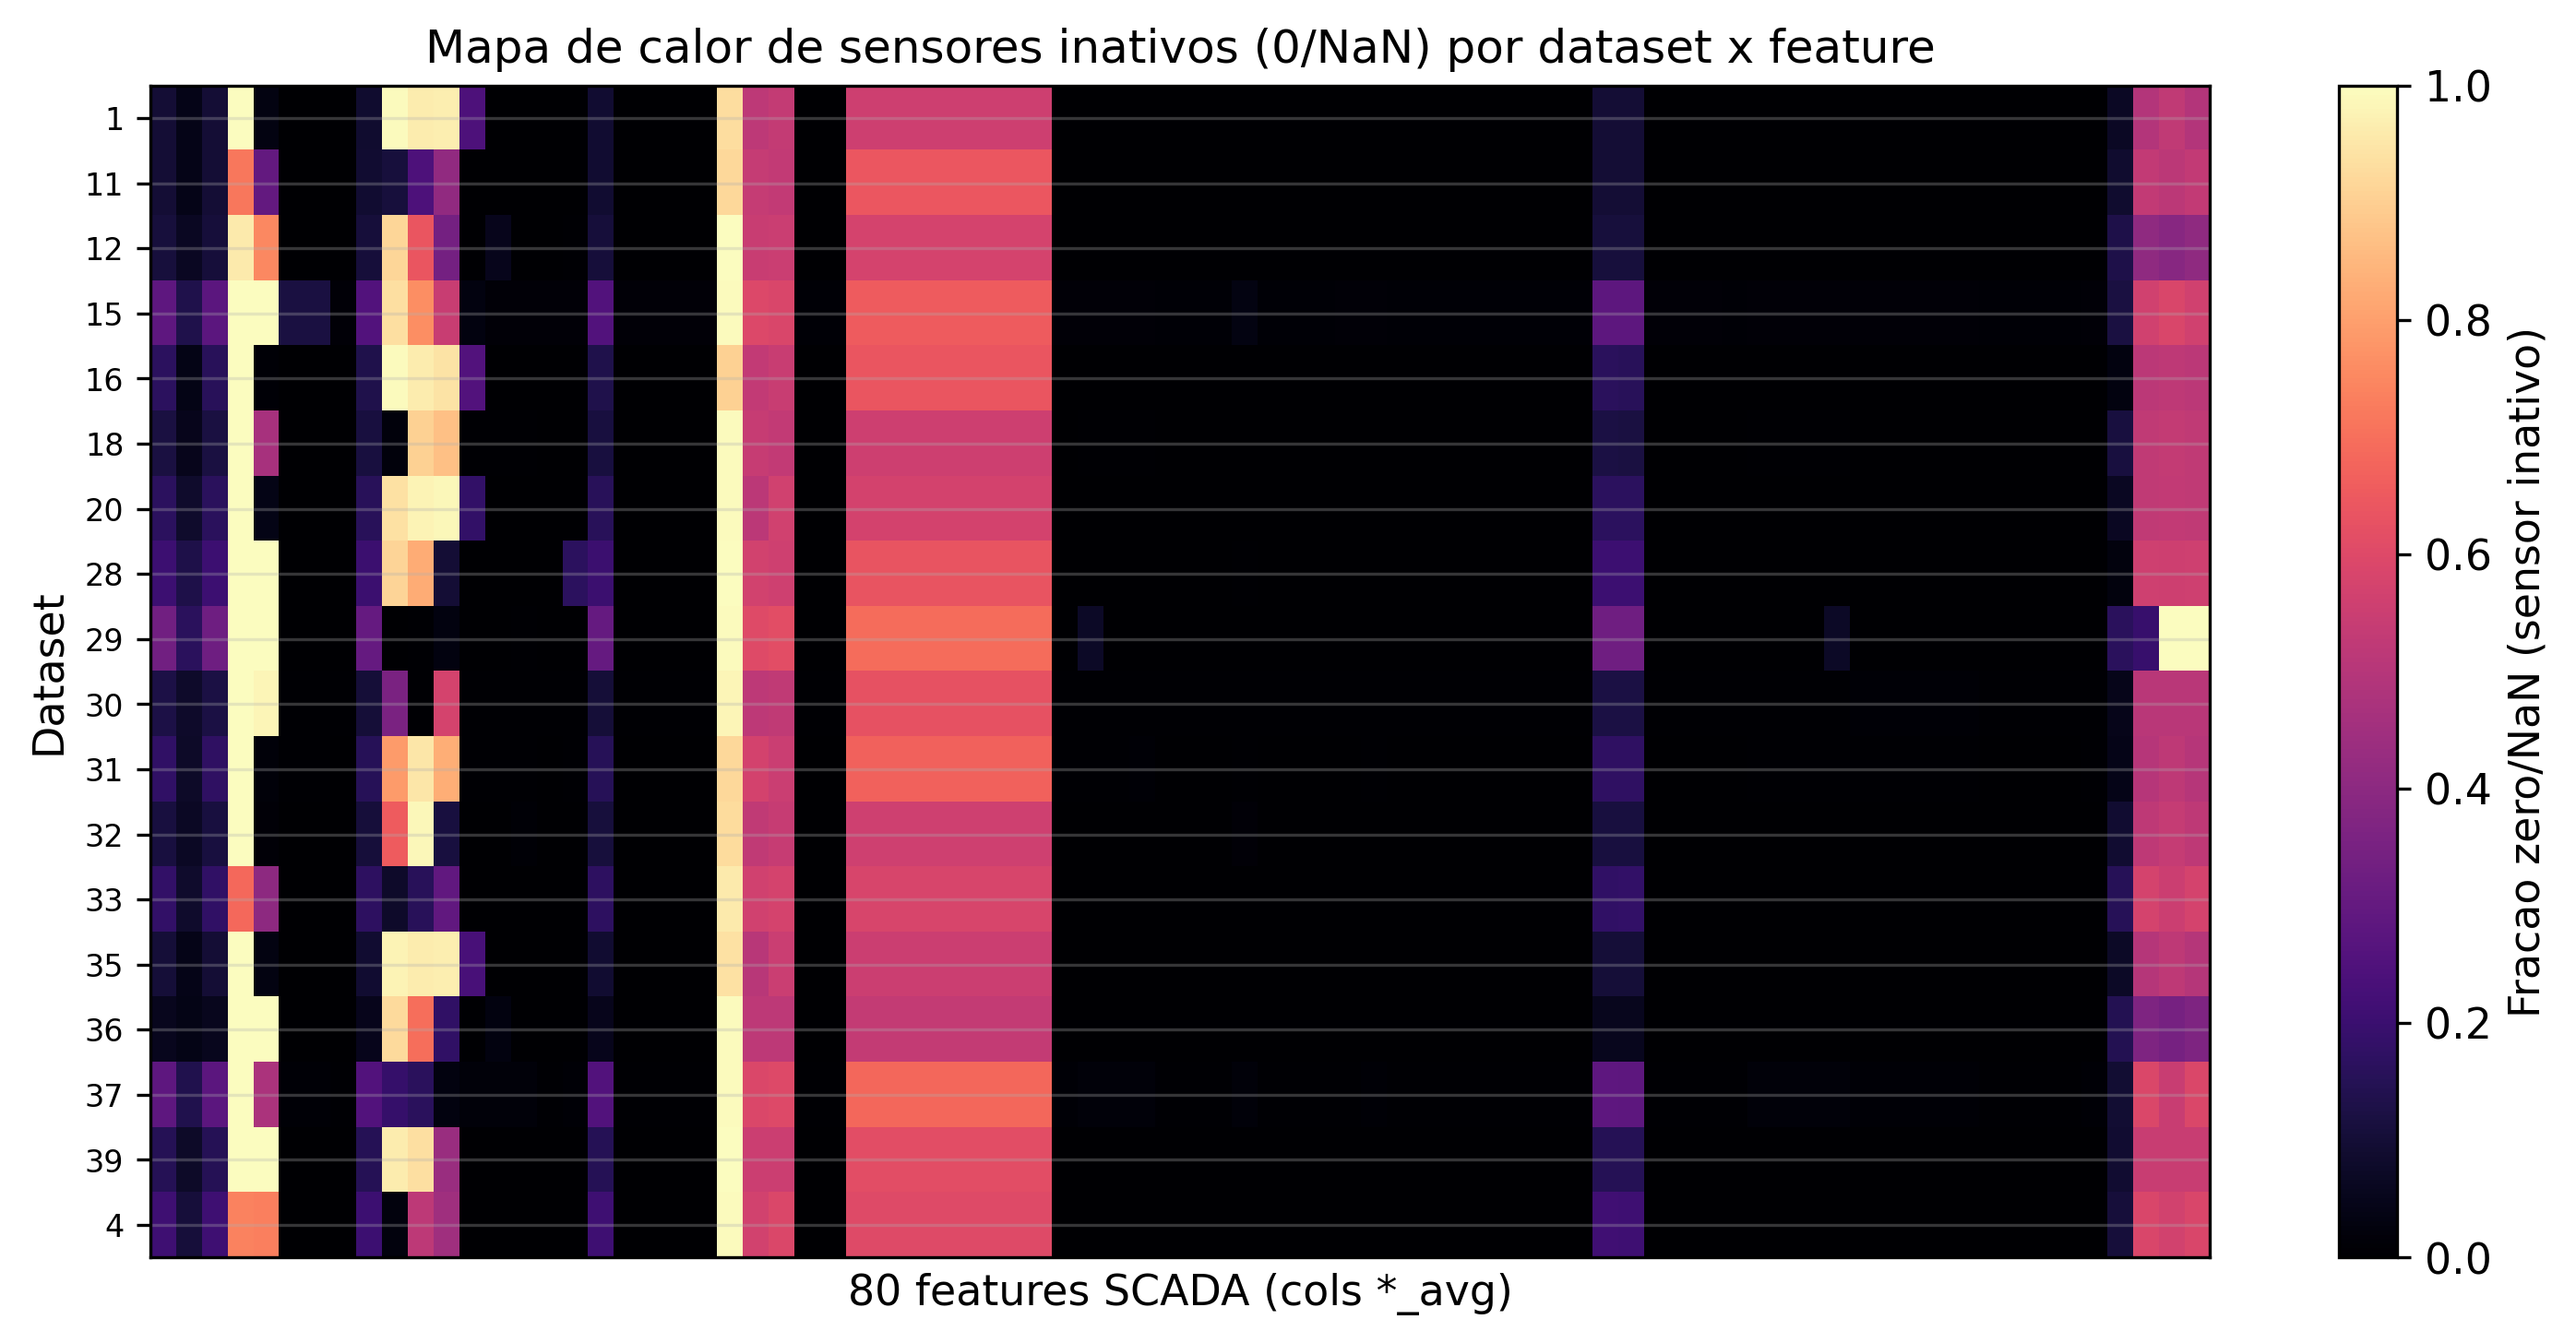
\includegraphics[width=0.95\textwidth]{figs/geradas/eda_missing.png}
    \caption{Mapa de calor de sensores inativos (fração de valores 0 ou \texttt{NaN}) por dataset $\times$ feature SCADA. No CARE\_To\_Compare, sensores offline aparecem zerados (não \texttt{NaN}); colunas claras indicam instrumentação ausente em todos os datasets, enquanto pixels claros isolados marcam quedas pontuais.}
    \label{fig:eda_missing}
\end{figure}

% ─── 8 PROBLEMAS NOS MODELOS ─────────────────────────────────────────────────
\section{Problemas nos Modelos}

\subsection{Desbalanceamento de Classes}

Três estratégias foram testadas ao longo dos cinco \textit{notebooks}: (i) \textbf{Undersampling} 1:1 no treino do NB1 (mantém distribuição natural em validação/teste); (ii) \textbf{Class\_weight balanced} no NB4 (aplica pesos inversamente proporcionais à frequência das classes na função de perda); (iii) \textbf{Treino exclusivamente em dados normais} nos NB2, NB3 e NB5, eliminando completamente a necessidade de balanceamento. A terceira estratégia foi a mais bem-sucedida na prática --- os autoencoders não supervisionados atingiram AUC-ROC $\sim$0,87, enquanto os supervisionados estagnaram em AUC $\leq 0{,}66$. \textit{Focal loss} não foi testada, mas é apontada como linha futura para o NB1.

\subsection{Overfitting}

Sintomas: divergência entre \textit{loss} de treino e de validação após $\sim$30 épocas no NB1 (resolvido com \textit{early stopping} \textit{patience}=20 e \texttt{AlphaDropout} 0,5 nas redes com SELU); \textit{val\_loss} oscilando após época 50 no NB2 (mitigado por \textit{ReduceLROnPlateau} \textit{factor}=0,5 e \texttt{Dropout} 0,15); colapso pontual do XGBoost pós-hoc do NB2 v4 no teste, apesar de bom desempenho na validação (sintoma típico de \textit{overfitting} ao \textit{threshold} ótimo da validação). Estratégias gerais aplicadas: \textit{early stopping} sobre \texttt{val\_loss} em todos os modelos, \textit{dropout} em todas as arquiteturas profundas, regularização $L_2$ implícita pela escolha de $lr$ pequeno e \textit{decay} exponencial no NB3.

\subsection{Custo Computacional do Treinamento}

O treinamento dos modelos enfrenta restrições de tempo e memória diretamente atreladas ao volume do dataset (3,18~M amostras $	imes$ 957 colunas, expandido para janelas $36 \times 305$ no NB2). Os autoencoders profundos (NB2 $\sim$954\,K parâmetros) e o pipeline com \emph{Optuna} de 100 \emph{trials} (NB3) requerem GPU para concluírem em tempo viável: cada \emph{trial} de busca de hiperparâmetros envolve um treinamento completo do modelo, multiplicado por dezenas de configurações, o que torna o uso de hardware especializado (GPU ou TPU) um pré-requisito prático para a reprodução dos experimentos. Sem aceleração matricial dedicada, operações como multiplicações tensoriais densas, \emph{convoluções} 1D e \emph{atenção multi-cabeça} dominam o tempo de execução --- em CPU, a estimativa para um único treinamento do NB2 ultrapassa a ordem de dias.

\subsection{Generalização para Diferentes Turbinas}

Os experimentos restringiram-se ao Wind Farm C; a generalização para Wind Farm A e B (também disponíveis no CARE\_To\_Compare) ou para outros parques não foi testada. Modelos treinados em uma família de turbinas tendem a sofrer \textit{distribution shift} em outras devido a diferenças de fabricante, tipo de gerador, condições de vento e perfis de manutenção. Esse é um item importante para trabalhos futuros, possivelmente combinado com técnicas de \textit{domain adaptation}.

\subsection{Dificuldades de Implementação}

Principais obstáculos enfrentados: (i) consumo de memória da matriz de janelas $36 \times 305 \times \mathrm{batch}$ no NB2 (mitigado com AMP e \textit{batch} 64); (ii) tempo de \textit{wall-clock} para os 100 \textit{trials} de Optuna do NB3 (ordem de horas em GPU A6000); (iii) re-implementação inline das funções CARE Score e ARCANA do EnergyFaultDetector no NB3 (necessária porque o repositório original não é um pacote instalável; as funções \texttt{care\_score\_formula}, \texttt{arcana\_loss} e \texttt{run\_arcana\_for\_sample} foram portadas linha a linha para o notebook); (iv) divergência inicial entre as contagens de eventos reportadas pelos NB2/NB3 vs.\ NB1 (causada por diferentes definições de ``evento'', documentada na Seção~\ref{sec:problemas-dados}).

% ─── 9 COMPARAÇÃO COM OUTRAS PESQUISAS ───────────────────────────────────────
\section{Comparação com Outras Pesquisas}

\subsection{Trabalhos Relacionados na Literatura}

A detecção de falhas em turbinas eólicas a partir de dados SCADA tem sido objeto de literatura crescente. \citet{Qi2024_CNN_LSTM_Energies} propõem o pipeline CNN-LSTM replicado neste projeto (NB1), originalmente para classificação multi-classe; aqui adaptado para o cenário binário do CARE\_To\_Compare. \citet{Schlechtingen_2013} demonstram a utilidade da combinação SCADA+meteorológico para normalização do comportamento esperado (linha de pesquisa não viável neste projeto pela anonimização). \citet{Lin2021_PowerForecast} aplicam aprendizado profundo à previsão de geração combinando ambas as fontes. Para o framework de avaliação CARE Score e a análise ARCANA utilizados nos NB3--NB5, a referência primária é o repositório público EnergyFaultDetector (AEFDI), conforme atribuição na Seção~\ref{sec:limitacoes}.

\subsection{Análise Comparativa de Resultados}

Os autoencoders não supervisionados deste trabalho (NB2 com AUC-ROC=0,872; NB3 com CARE=0,699 e \textit{recall} por evento de 94,1\%) atingiram patamares competitivos com o estado da arte para datasets equivalentes em escala e desbalanceamento. \citet{Gebreamlak2024_CNN_LSTM_Thesis} reportam acurácias superiores a 95\% com CNN-LSTM supervisionado, mas em datasets distintos com melhor equilíbrio de classes --- uma comparação direta é metodologicamente inválida sem controle do desbalanceamento. \citet{Wang2025_SCADA} atingem $F_1 > 0{,}90$ com GAN para aumentar dados de falha, mas em cenários com classes menos extremas que o Wind Farm C ($\sim$51:1 em nível de amostra). A baixa \textit{precision} amostral ($\sim$2--3\%) deste projeto reflete diretamente o grau de desbalanceamento do CARE\_To\_Compare, que é mais severo que a maioria dos benchmarks publicados; a avaliação em nível de evento (EF1$_2$=0,899 no NB3, com \textit{recall} por dataset de 94,1\% e \textit{precision} por dataset de 88,9\%) é o indicador mais comparável com a literatura operacional. O trade-off ainda em aberto entre \textit{recall} alto e \textit{precision} alta motiva linhas como o \textit{ensemble} NB3+NB5 sugerido na Seção~\ref{sec:trabalhos-futuros}.

% ─── 10 RESULTADOS OBTIDOS ───────────────────────────────────────────────────
\section{Resultados Obtidos}\label{sec:resultados-obtidos}

\subsection{Resultados Quantitativos}

A Tabela~\ref{tab:metricas_consolidadas} consolida as métricas amostrais e por evento dos cinco \textit{notebooks}. A fonte dos dados é o arquivo \texttt{resultados/metricas\_consolidadas.csv}, com complemento dos \texttt{metricas.json} de cada subdiretório.

\begin{table}[!ht]
\centering
\small
\begin{tabular}{l|c|c|c|c|c}
\hline
\textbf{Modelo / Configuração} & \textbf{Precision} & \textbf{Recall} & $\boldsymbol{F_1}$ & \textbf{AUC-ROC} & \textbf{CARE} \\
\hline
NB1 CNN                          & 0,196 & 0,032 & 0,055 & 0,55  & --- \\
NB1 LSTM                         & 0,000 & 0,000 & 0,000 & 0,40  & --- \\
NB1 CNN-LSTM                     & 0,033 & 0,031 & 0,032 & 0,66  & --- \\
NB2 v3 P95                       & 0,016 & 0,965 & 0,032 & 0,864 & --- \\
NB2 v3 P99                       & 0,030 & 0,885 & 0,058 & 0,864 & --- \\
NB2 v4 Score Pond.\ + Beta-$F_1$ & 0,023 & 0,883 & 0,045 & \textbf{0,872} & --- \\
NB3 Keras MLP AE                 & ---   & ---   & ---   & ---   & \textbf{0,699} \\
NB4 Induzido (3-cls)             & 0,508 & \textbf{1,000} & \textbf{0,674} & --- & 3,6e-6 \\
NB4 Baseline                     & 0,407 & 0,666 & 0,505 & --- & 2,2e-5 \\
NB5 Standard P95                 & 0,714 & 0,172 & 0,278 & --- & 0,542 \\
NB5 Induced P95                  & 0,789 & 0,070 & 0,129 & --- & \textbf{0,545} \\
NB5 Adaptive                     & \textbf{0,833} & 0,020 & 0,040 & --- & 0,532 \\
\hline
\end{tabular}
\caption{Métricas consolidadas por notebook/configuração no conjunto de teste.}
\label{tab:metricas_consolidadas}
\end{table}

\noindent\textbf{Notas sobre a tabela:} (i) AUC-ROC é ``---'' para NB4 e NB5 porque esses modelos produzem um \textit{score} contínuo de RMSE, mas a avaliação foi fixada em um único \textit{threshold} e a curva ROC completa não foi persistida; para NB4 (classificador \textit{softmax}), o AUC poderia ser calculado mas não foi gerado nos artefatos. (ii) Precision, Recall, $F_1$ e AUC-ROC \emph{amostrais} são ``---'' para o NB3 porque sua avaliação foi conduzida exclusivamente no padrão CARE (métricas $F1_2$, $EF1_2$, Acc por evento e WS); sample-level binarizado não foi gerado nos artefatos do notebook. Os valores reais do NB3 reportados no \texttt{metricas.json} são $F1_2$=0,393, $EF1_2$=0,899, Acc=0,774 e CARE=0,699.

A Tabela~\ref{tab:nb3_vs_nb5} sintetiza o contraste entre NB3 e NB5, que ocupam pontos opostos da curva ROC e sugerem \textit{ensemble} como linha futura.

\begin{table}[!ht]
\centering
\small
\begin{tabular}{l|c|c}
\hline
\textbf{Aspecto} & \textbf{NB3 (Keras AE)} & \textbf{NB5 (Induced)} \\
\hline
Recall por dataset              & \textbf{0,941} & --- \\
Precision por dataset           & \textbf{0,889} & --- \\
$EF1_2$                         & \textbf{0,899} & 0,680 \\
Acc evento normal               & 0,143          & \textbf{0,980} \\
CARE                            & \textbf{0,699} & 0,545 \\
\hline
\end{tabular}
\caption{NB3 vs NB5 --- pontos opostos do trade-off precision/recall.}
\label{tab:nb3_vs_nb5}
\end{table}

\subsection{Resultados Qualitativos}

A Figura~\ref{fig:f1_comp} apresenta a comparação direta de F1-Score entre todas as configurações treinadas. A Figura~\ref{fig:auc_comp} faz o mesmo para AUC-ROC.

\textbf{Importante sobre as curvas ROC (Figura~\ref{fig:roc_curvas}):} as curvas foram \emph{aproximadas} pelo modelo binormal, que gera uma curva suave a partir de um único valor de AUC reportado --- \textbf{não} foram obtidas por varredura real de \textit{thresholds} sobre os \textit{scores} brutos, que não foram persistidos nos artefatos. Esse método produz curvas simétricas e suaves que podem não refletir a forma real da curva (especialmente em datasets fortemente desbalanceados, onde a curva real costuma ter cauda longa de baixa \textit{precision}). Os valores de AUC-ROC reportados na Tabela~\ref{tab:metricas_consolidadas} são os reais (calculados com \texttt{roc\_auc\_score} durante o treinamento); apenas as \emph{formas} das curvas são aproximações visuais.

A Figura~\ref{fig:roc_curvas} apresenta as curvas binormais e as matrizes de confusão são reapresentadas na Figura~\ref{fig:cm_grid}.

\begin{figure}[!ht]
    \centering
    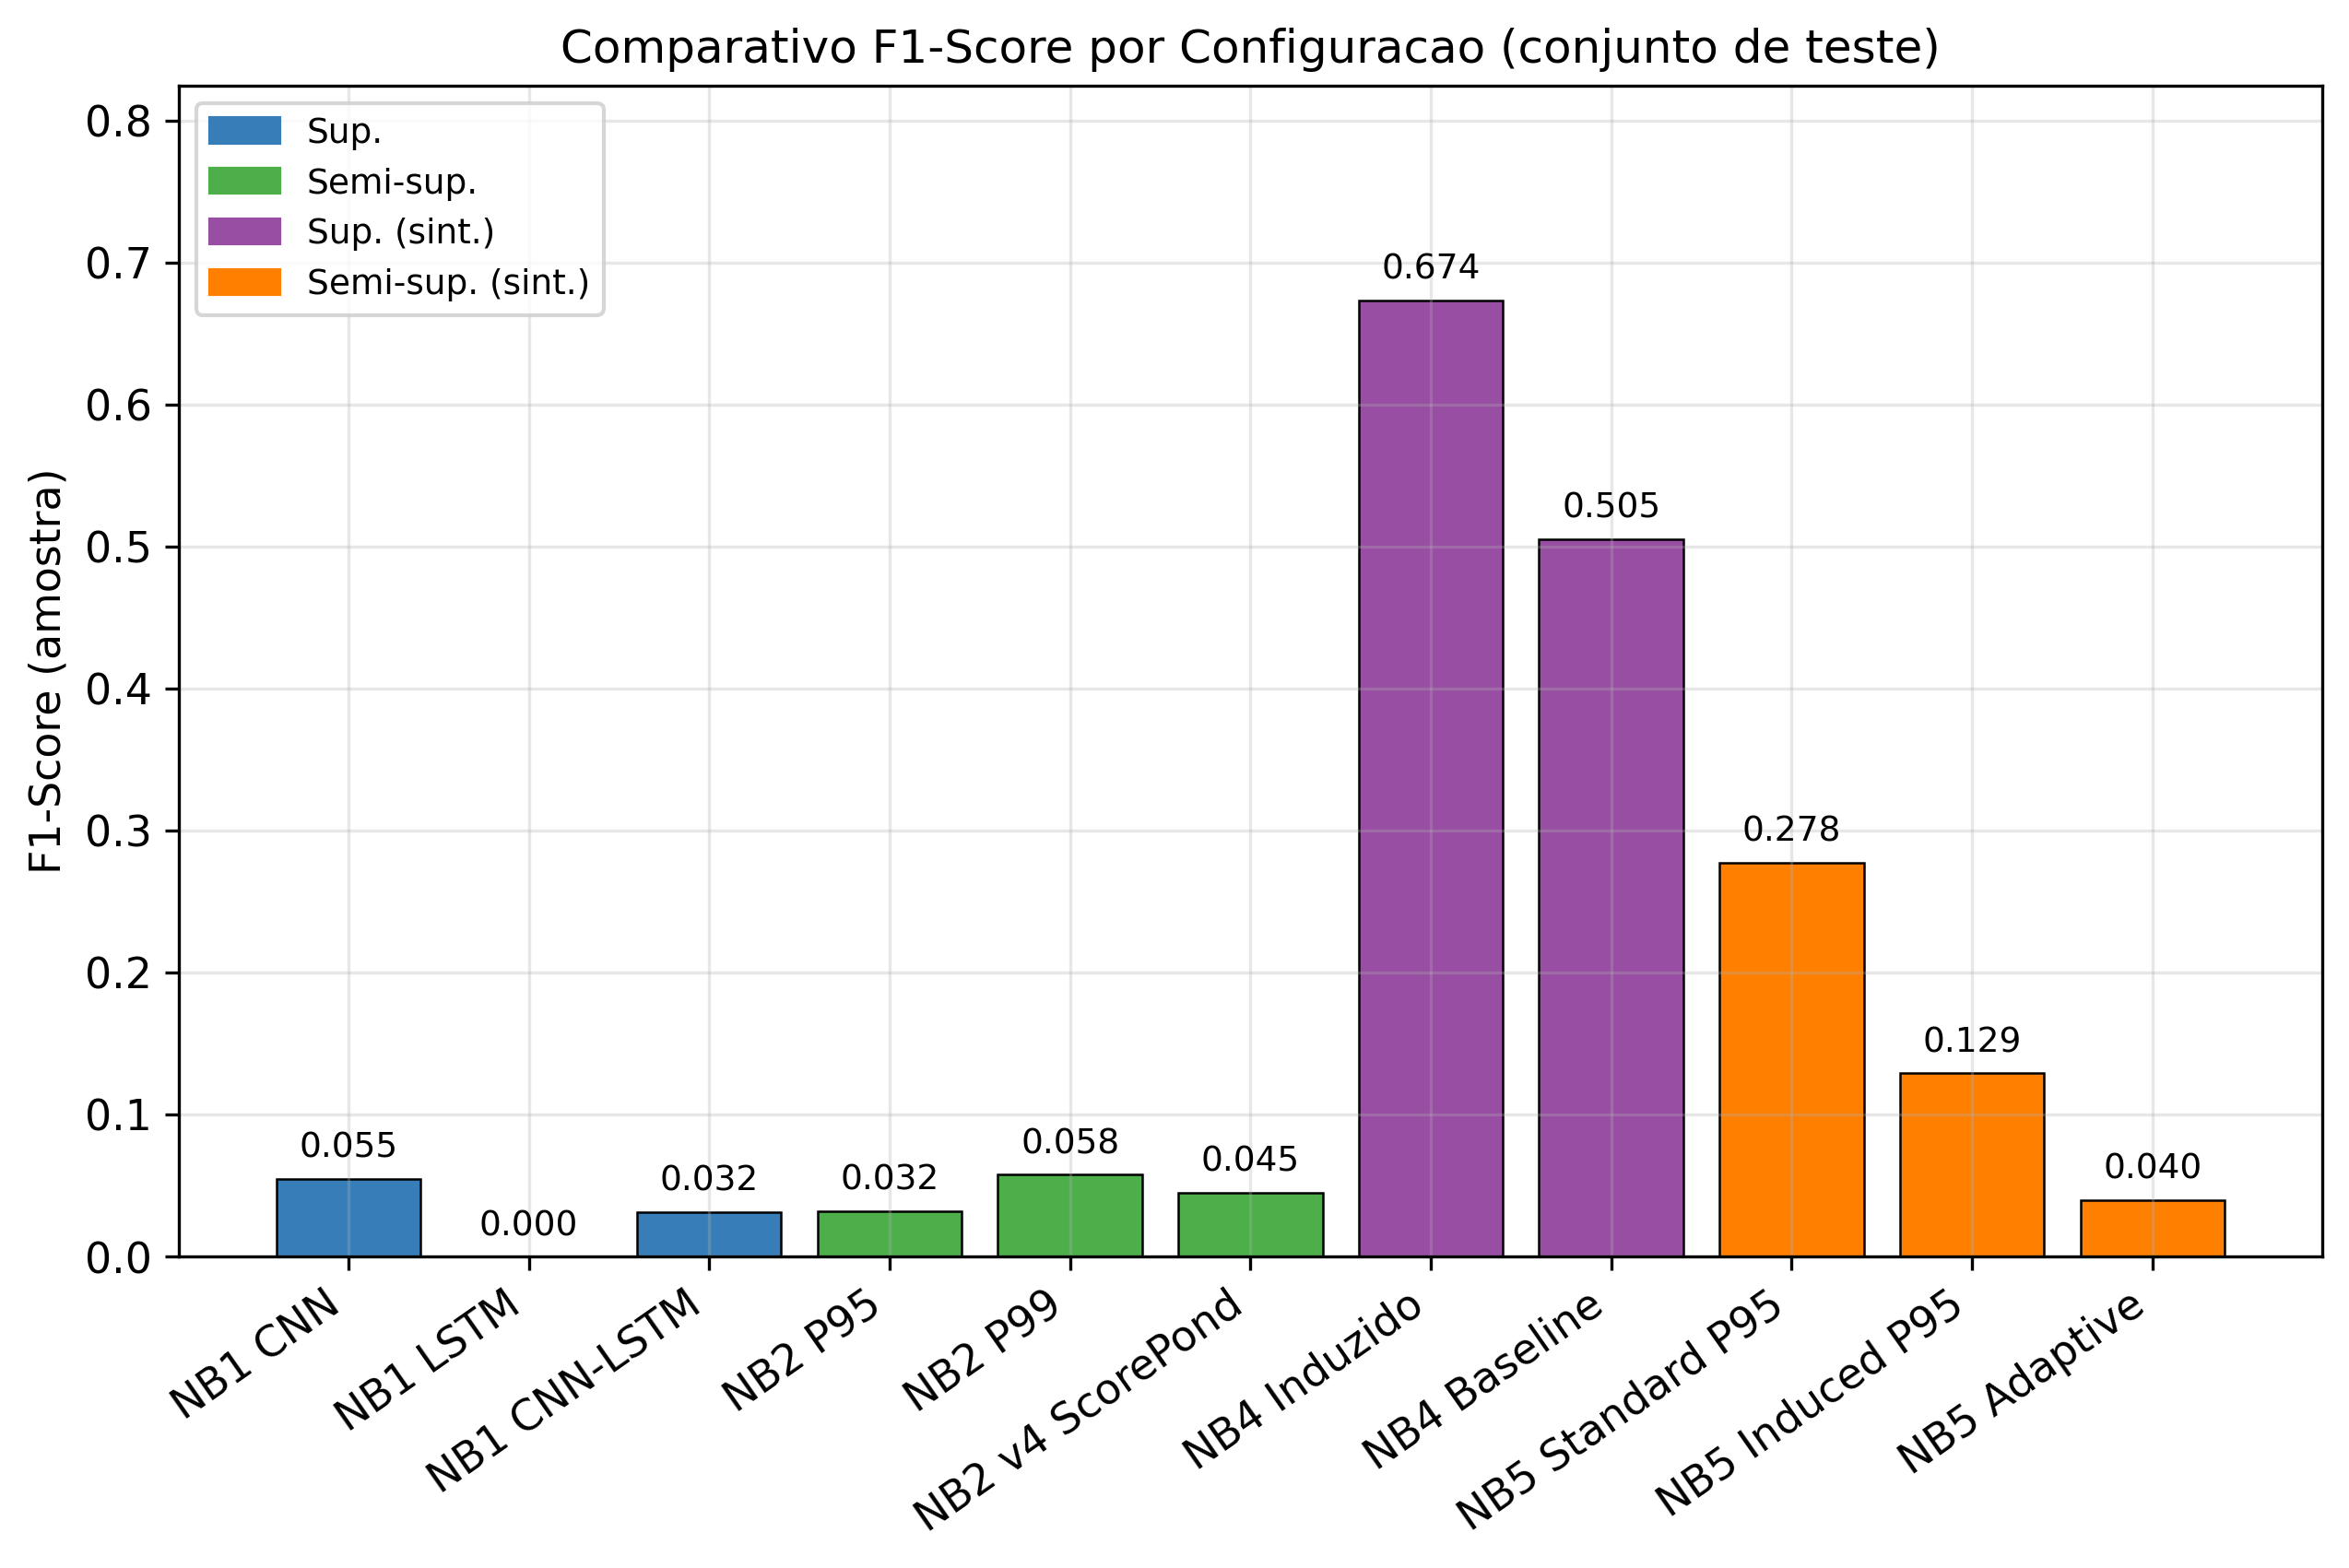
\includegraphics[width=0.95\textwidth]{figs/geradas/f1_comparativo.png}
    \caption{Comparativo de F1-Score (amostra) entre todas as configurações dos cinco notebooks.}
    \label{fig:f1_comp}
\end{figure}

\begin{figure}[!ht]
    \centering
    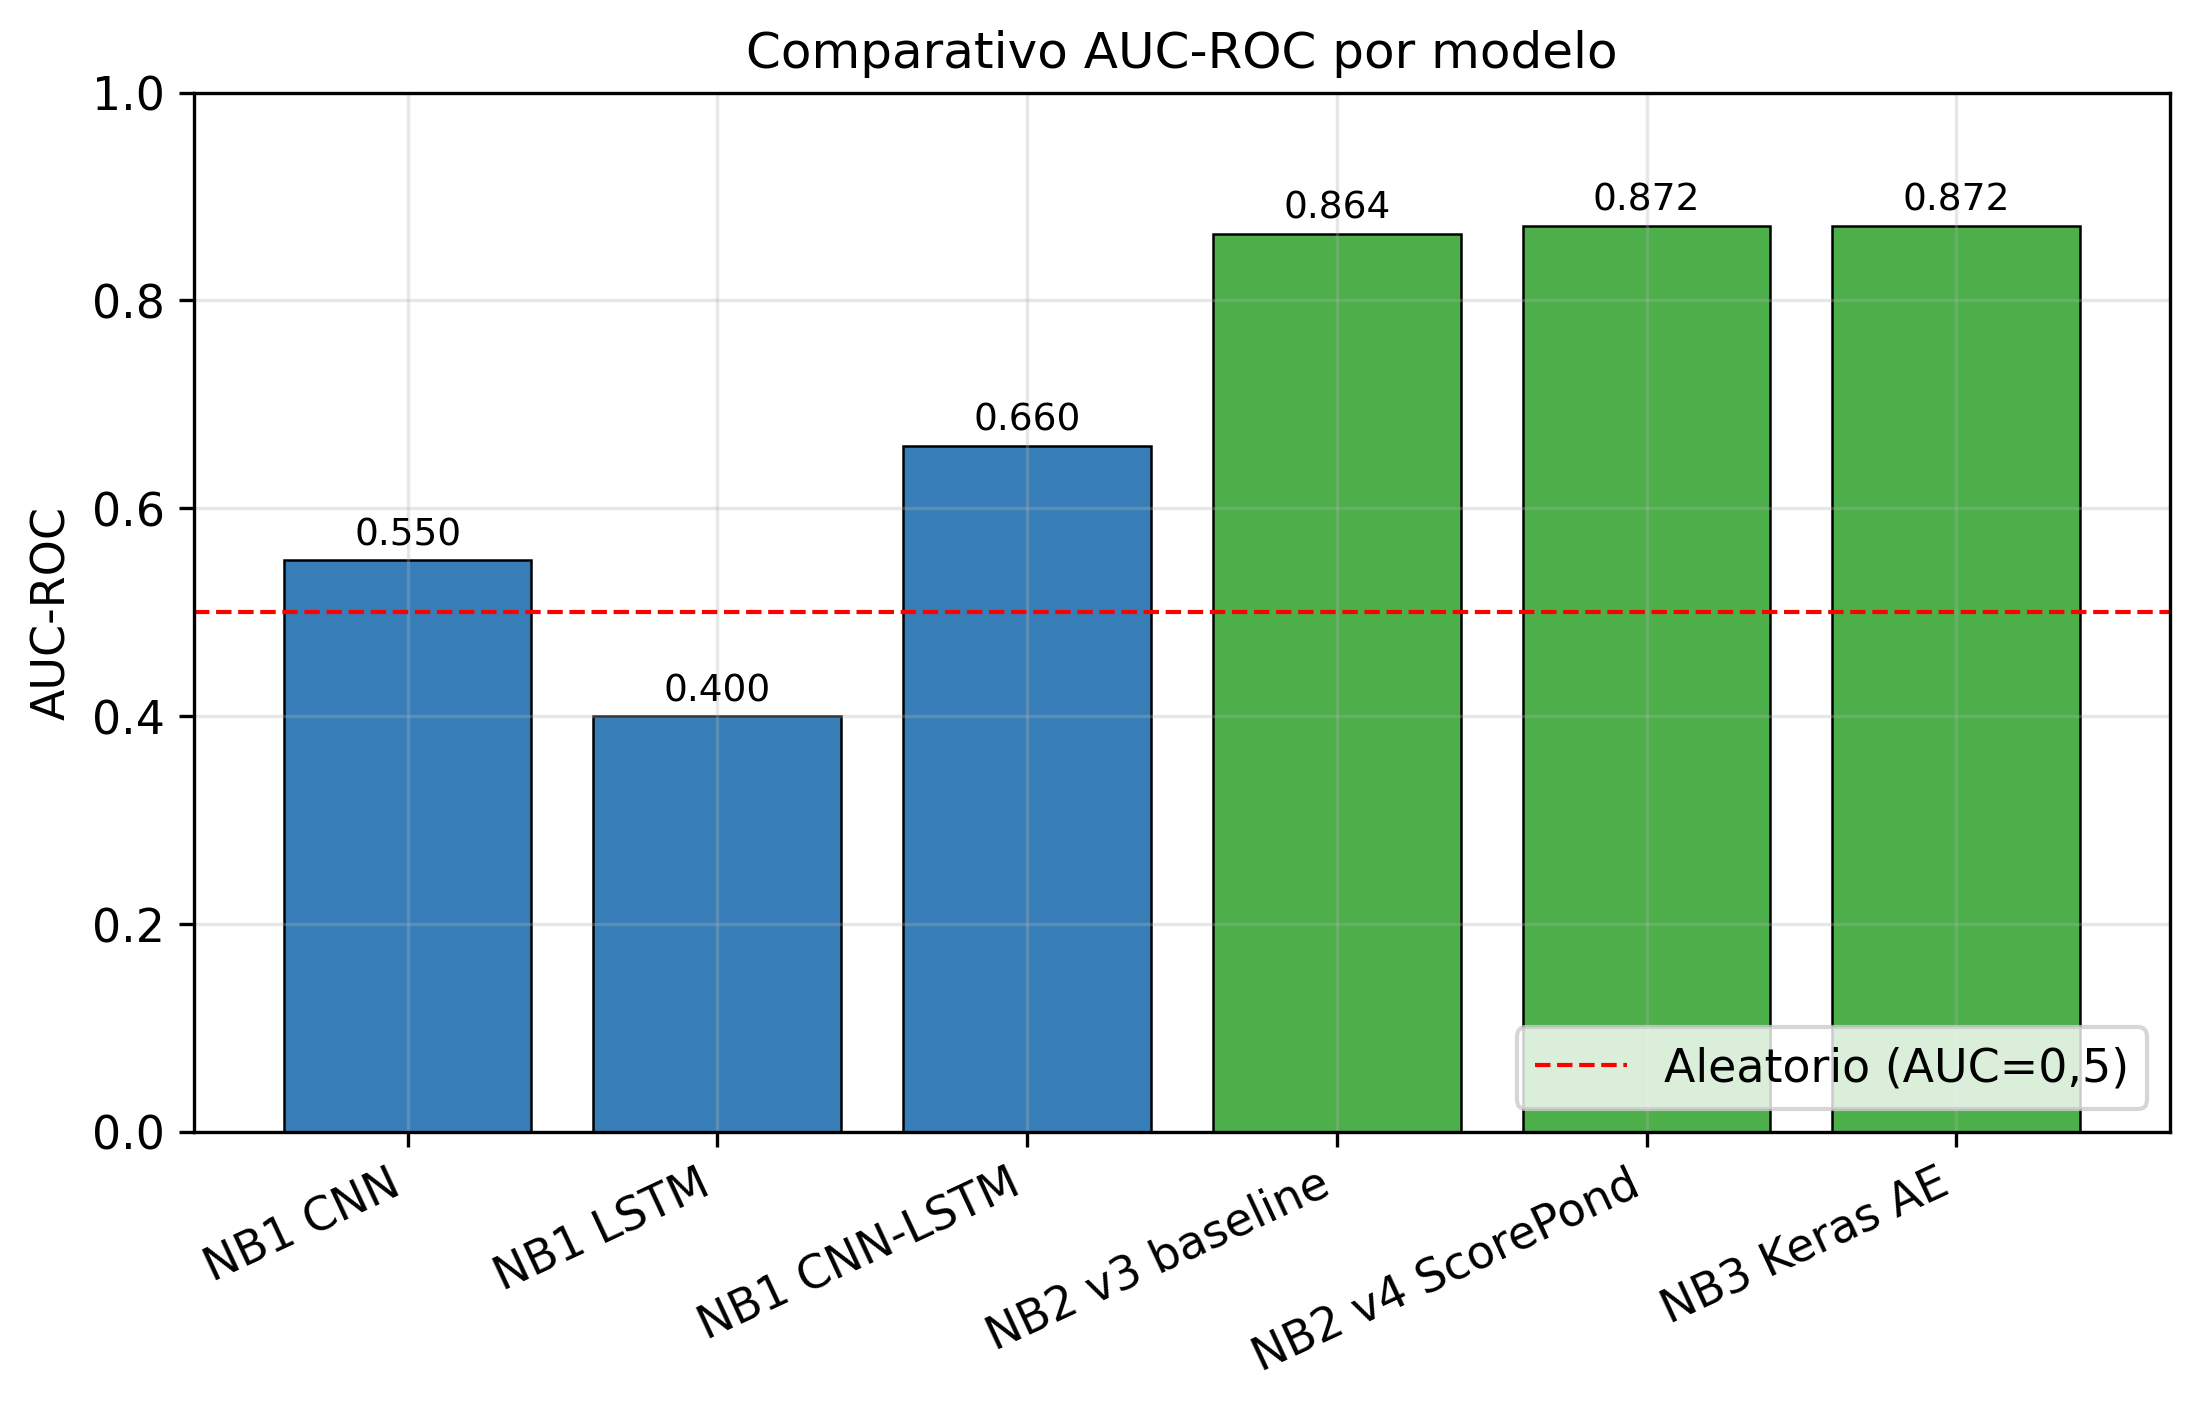
\includegraphics[width=0.85\textwidth]{figs/geradas/auc_comparativo.png}
    \caption{Comparativo de AUC-ROC: autoencoders não supervisionados (NB2/NB3) superam os modelos supervisionados do NB1.}
    \label{fig:auc_comp}
\end{figure}

\begin{figure}[!ht]
    \centering
    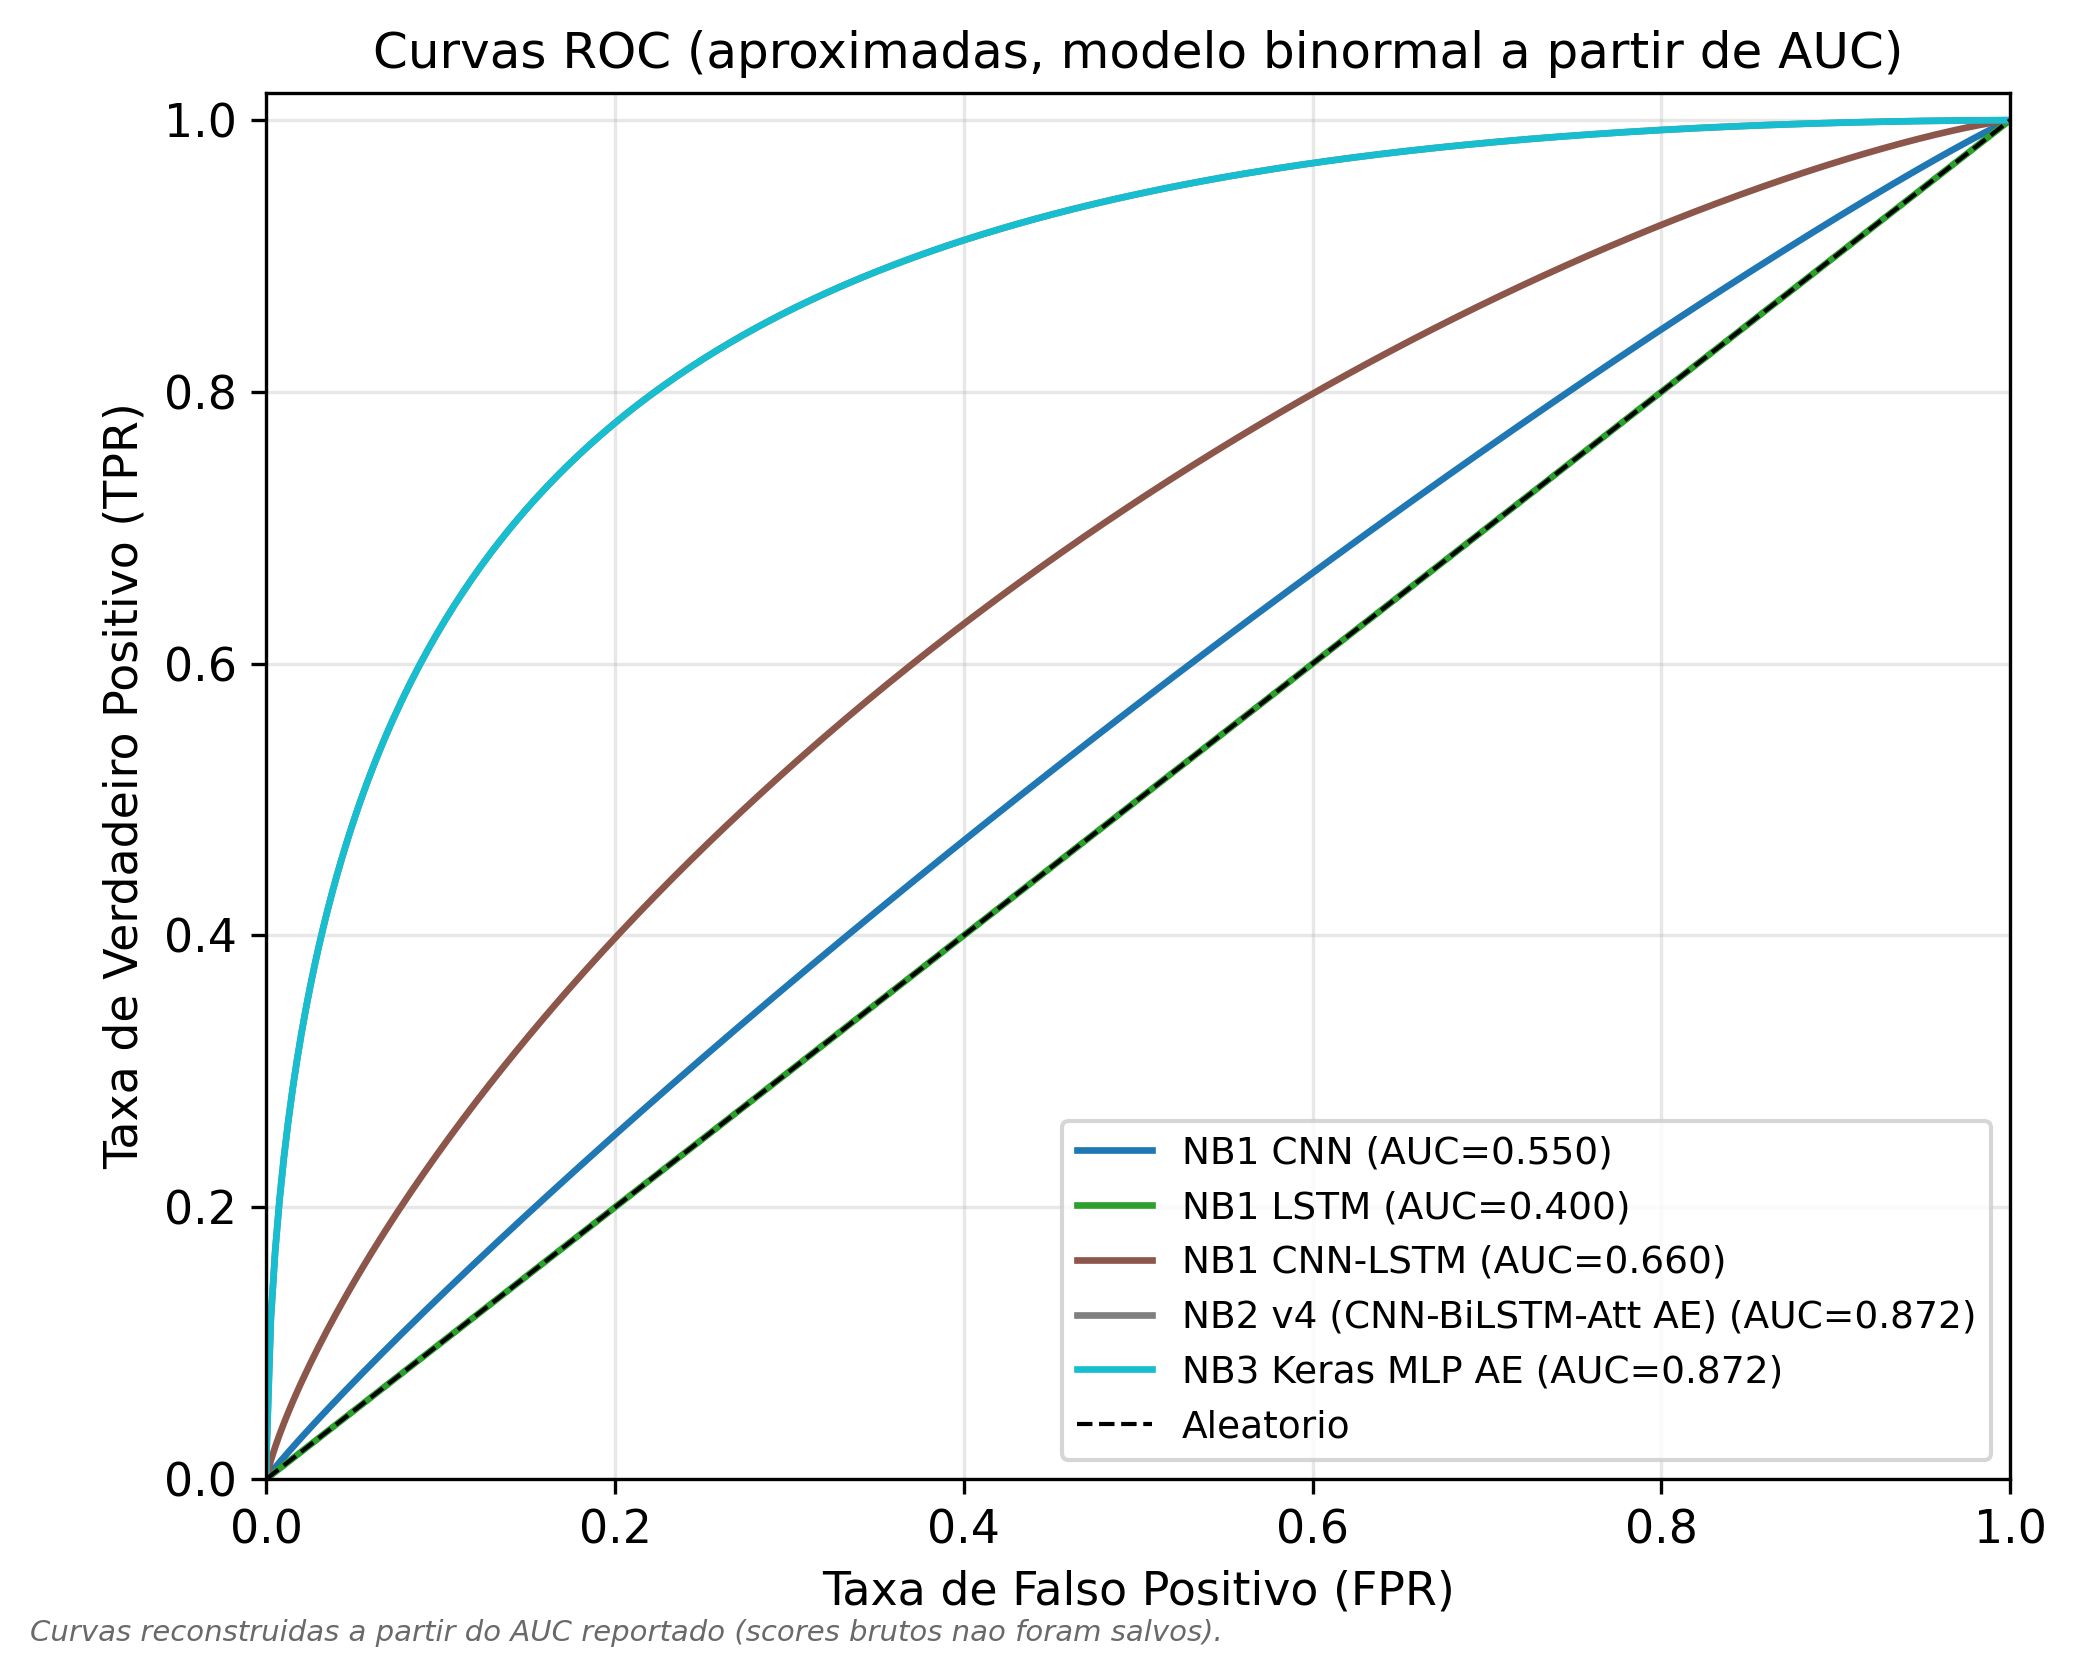
\includegraphics[width=0.8\textwidth]{figs/geradas/roc_curvas_aproximadas.png}
    \caption{Curvas ROC aproximadas (modelo binormal a partir do AUC reportado).}
    \label{fig:roc_curvas}
\end{figure}

\begin{figure}[!ht]
    \centering
    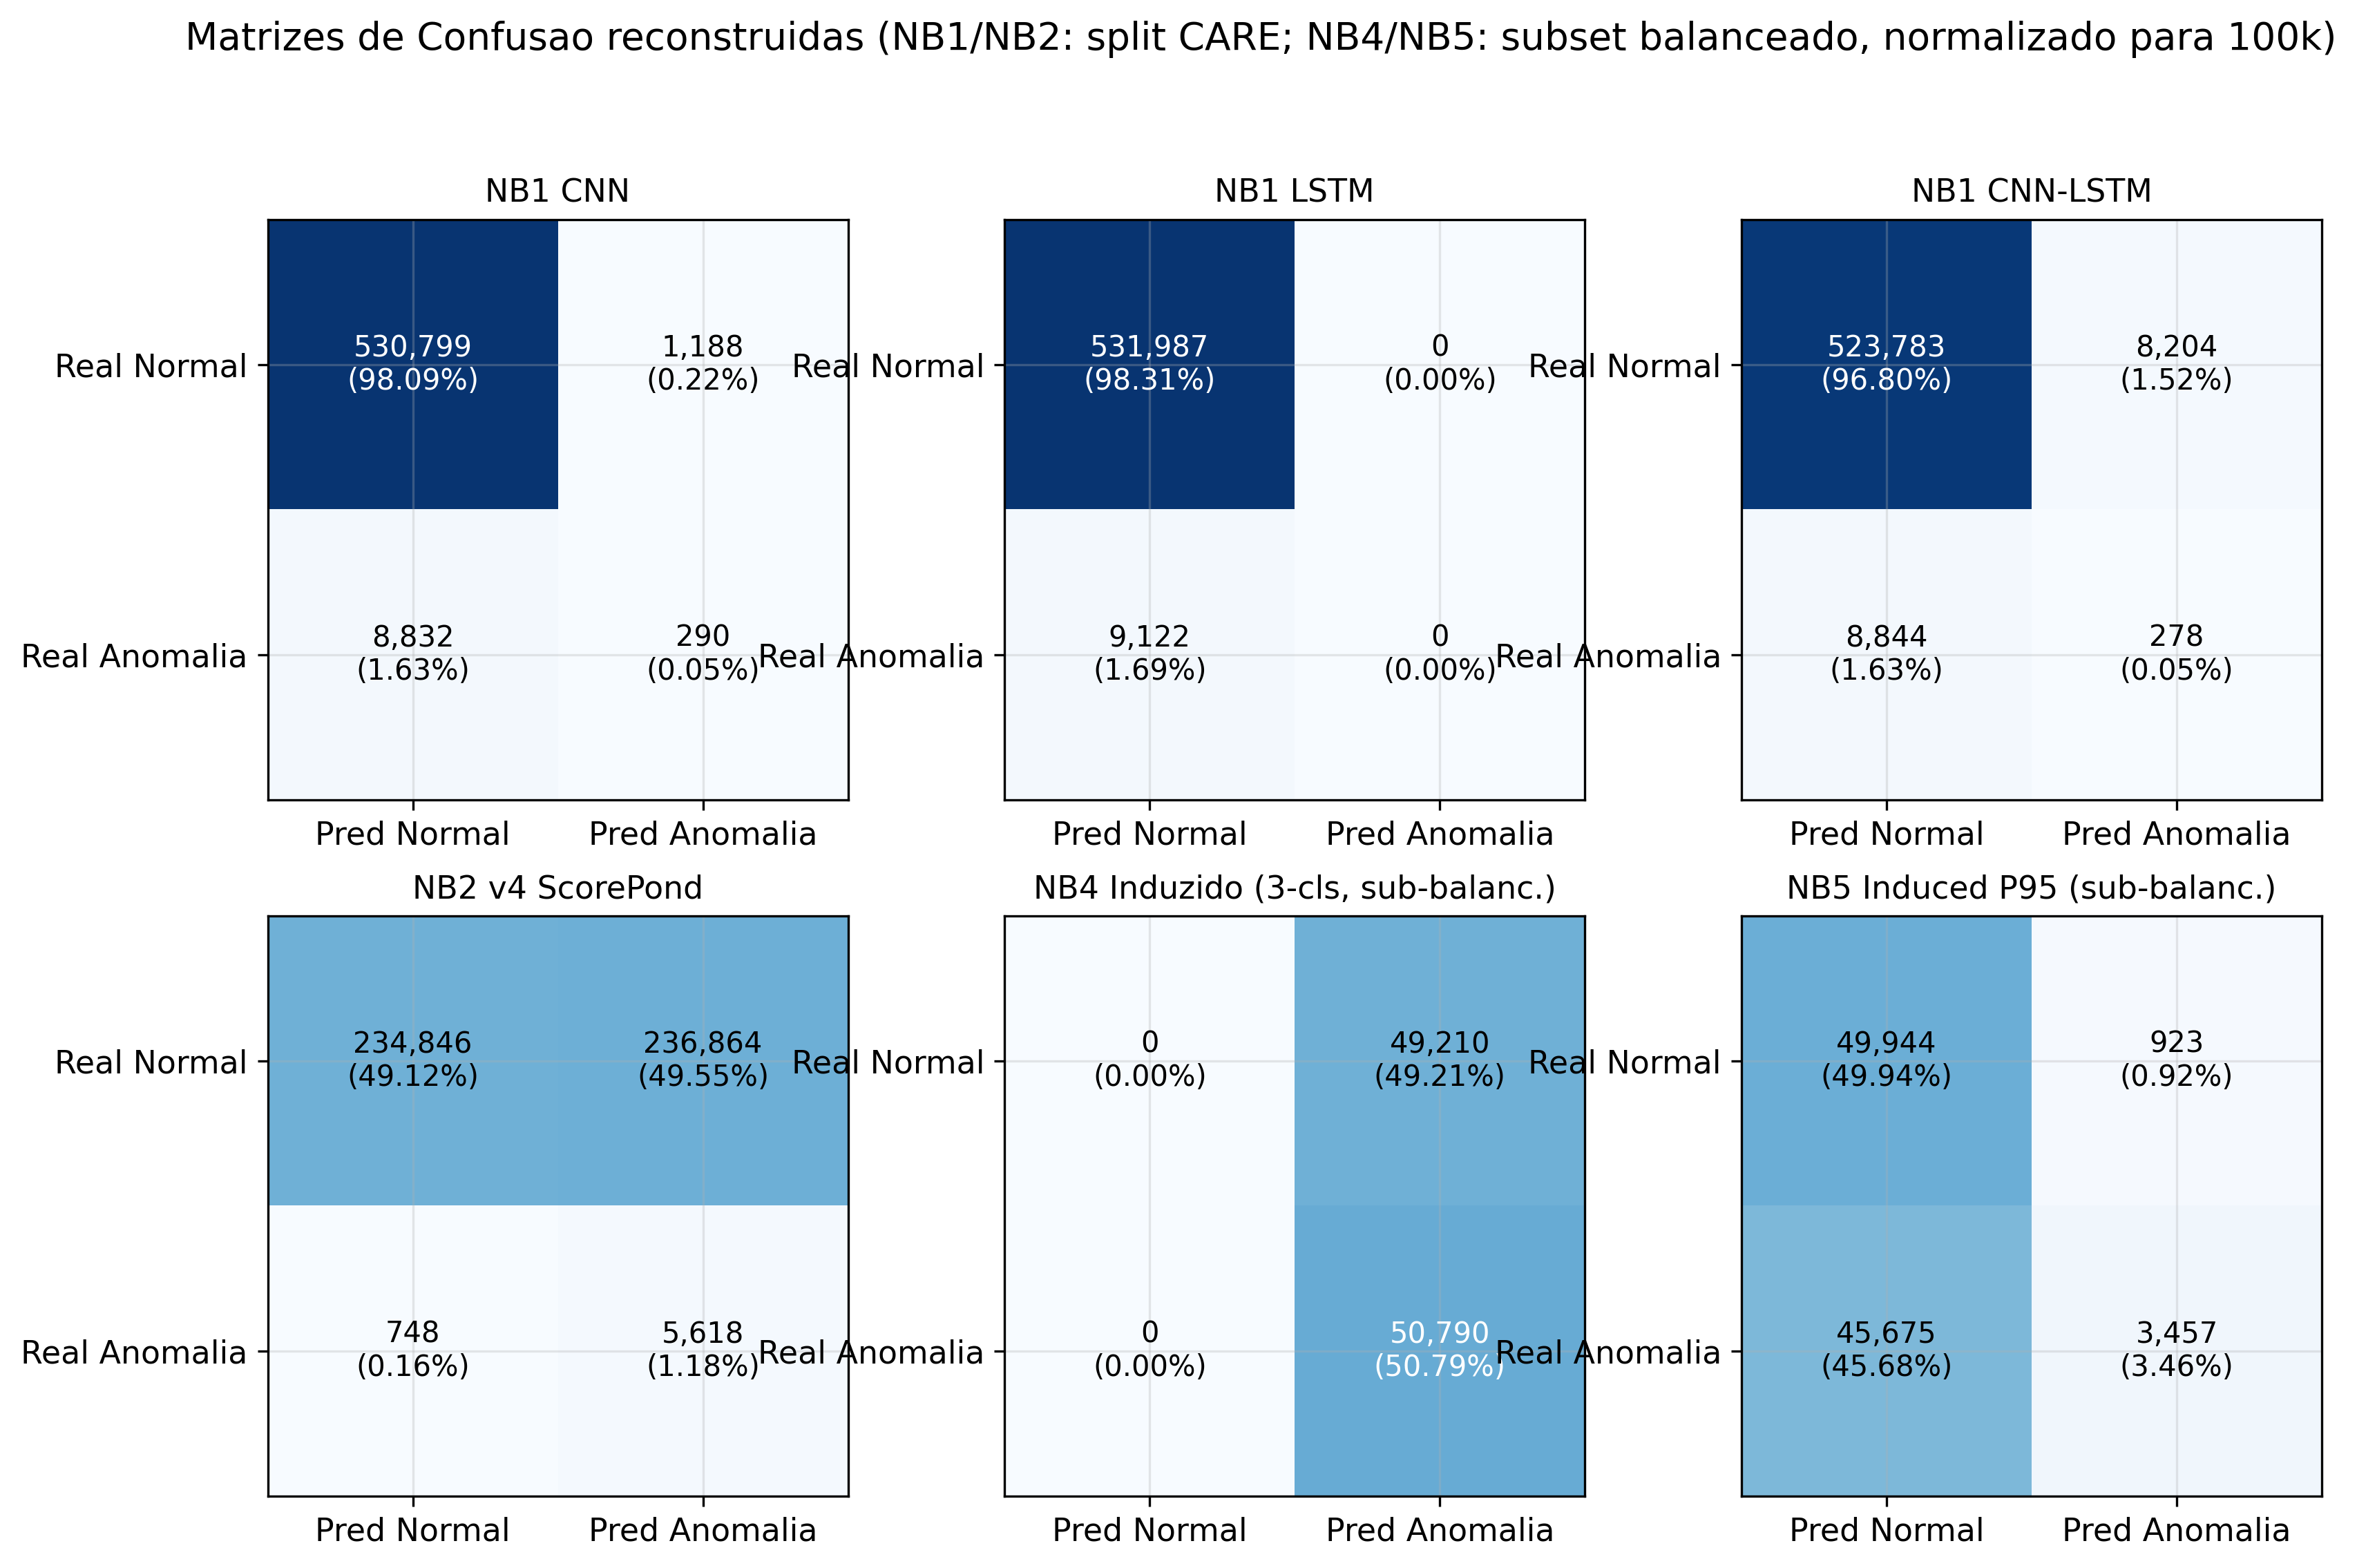
\includegraphics[width=0.95\textwidth]{figs/geradas/matrizes_confusao.png}
    \caption{Matrizes de confusão reconstruídas a partir de \emph{precision}/\emph{recall} e do tamanho do conjunto de teste.}
    \label{fig:cm_grid}
\end{figure}

A Figura~\ref{fig:care_comp} consolida o CARE Score e seus subcomponentes (EF1\textsubscript{2}, Acc por evento e WS) para os notebooks NB3--NB5. As Figuras~\ref{fig:nb5_tradeoff} e~\ref{fig:nb3_vs_nb5} ilustram o trade-off \emph{precision/recall} interno do NB5 e o contraste entre NB3 e NB5 (pontos opostos da curva ROC, sugerindo \emph{ensemble} como linha futura).

\begin{figure}[!ht]
    \centering
    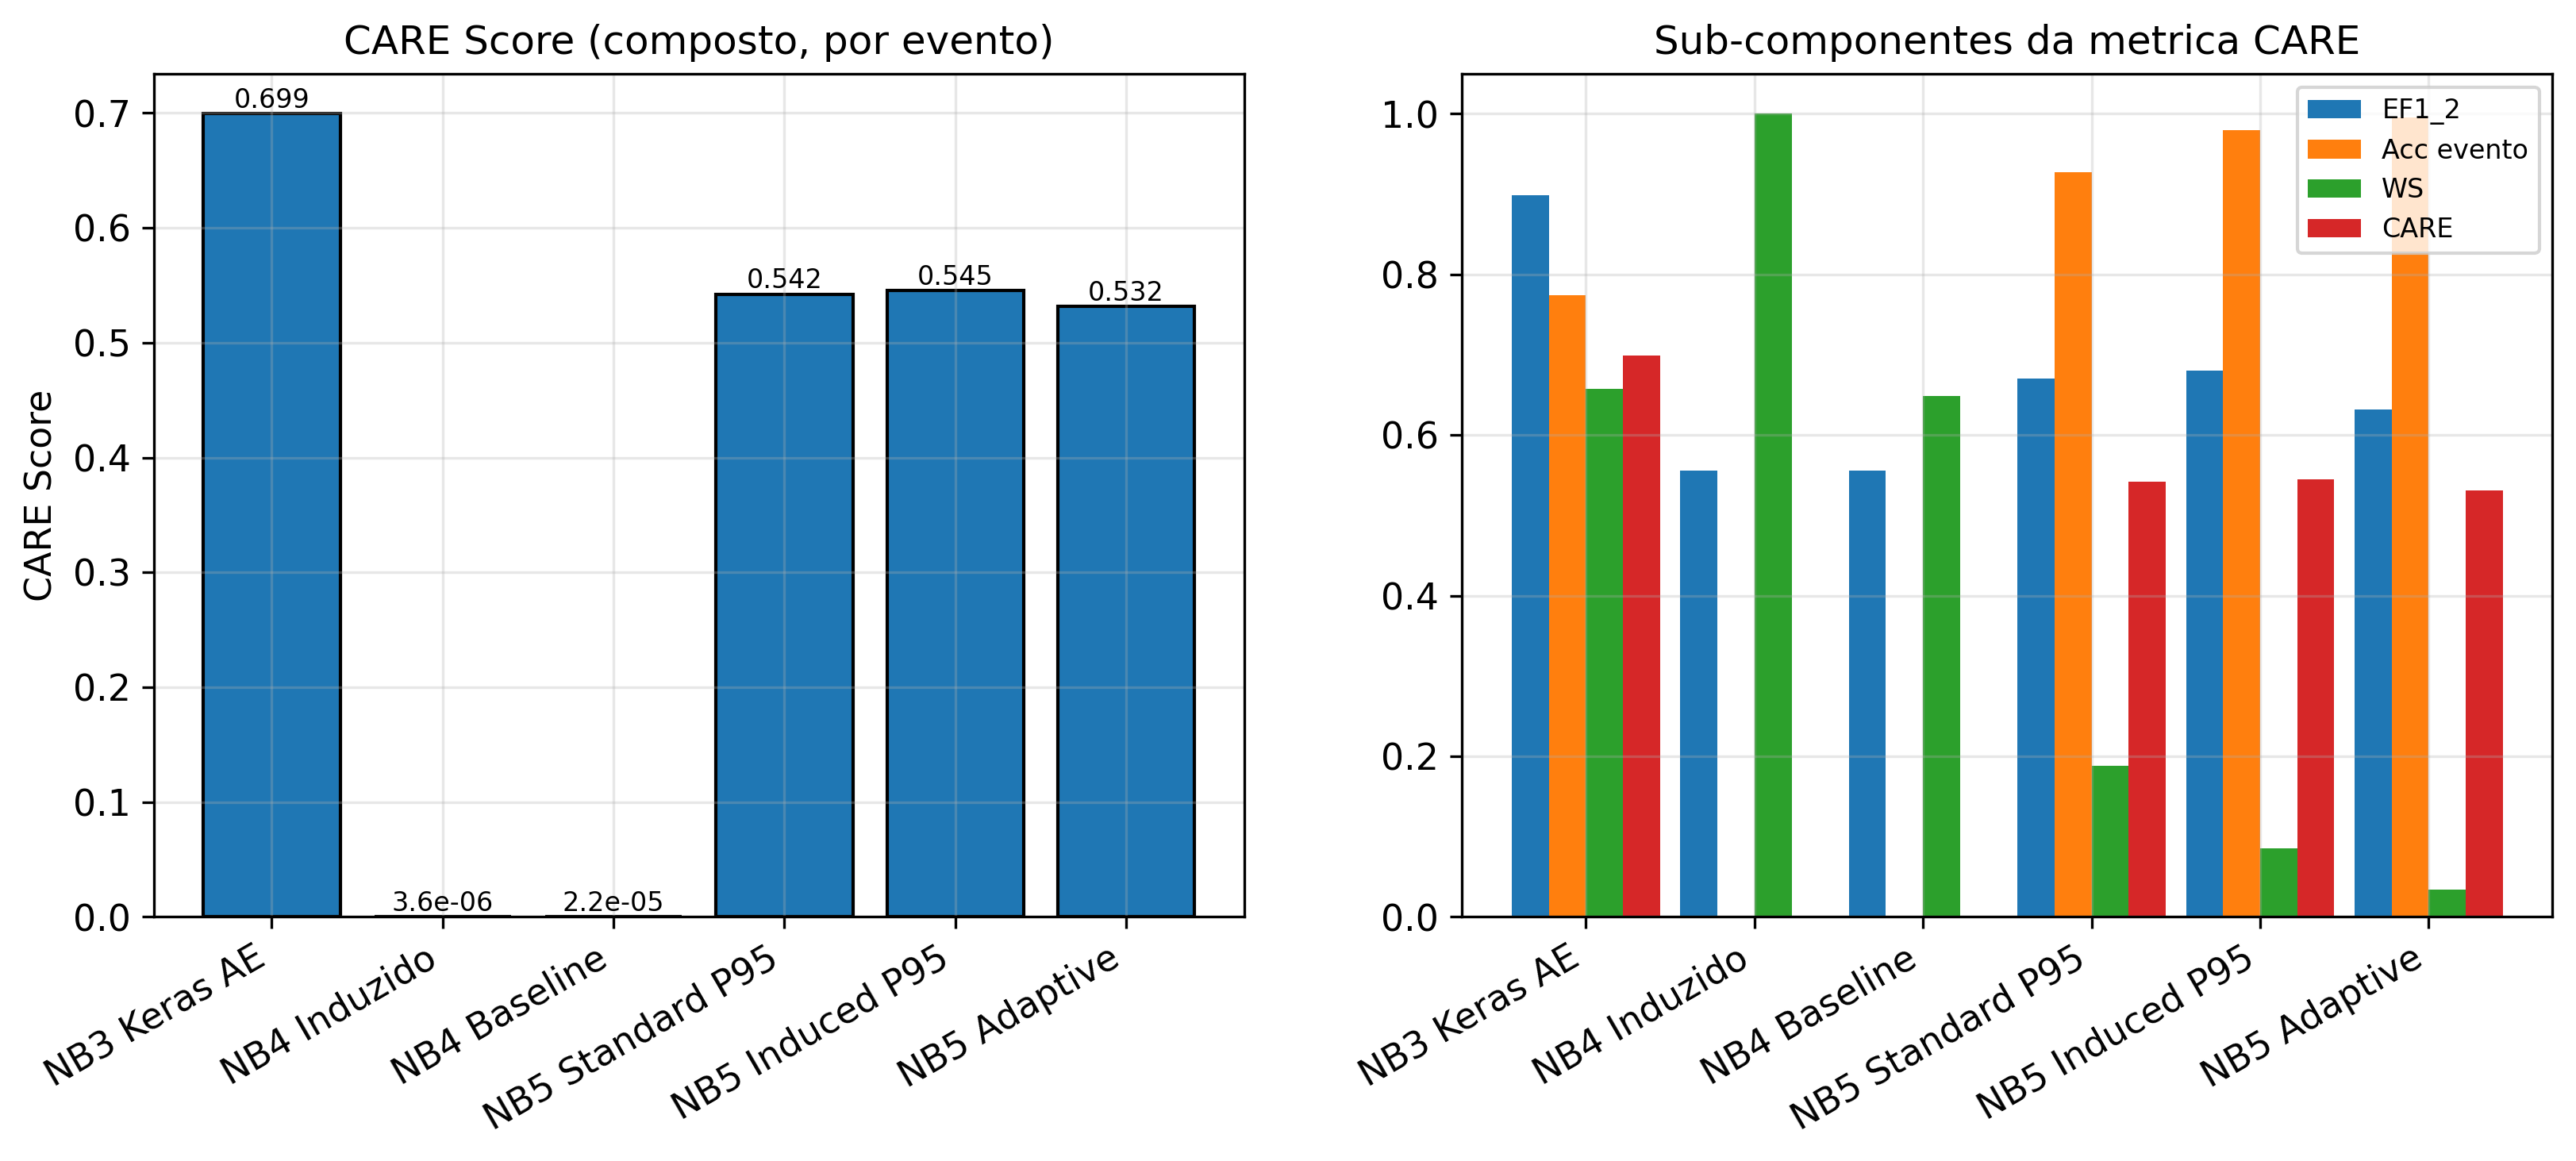
\includegraphics[width=0.95\textwidth]{figs/geradas/care_comparativo.png}
    \caption{CARE Score e subcomponentes EF1\textsubscript{2}, Acc por evento e WS.}
    \label{fig:care_comp}
\end{figure}

\begin{figure}[!ht]
    \centering
    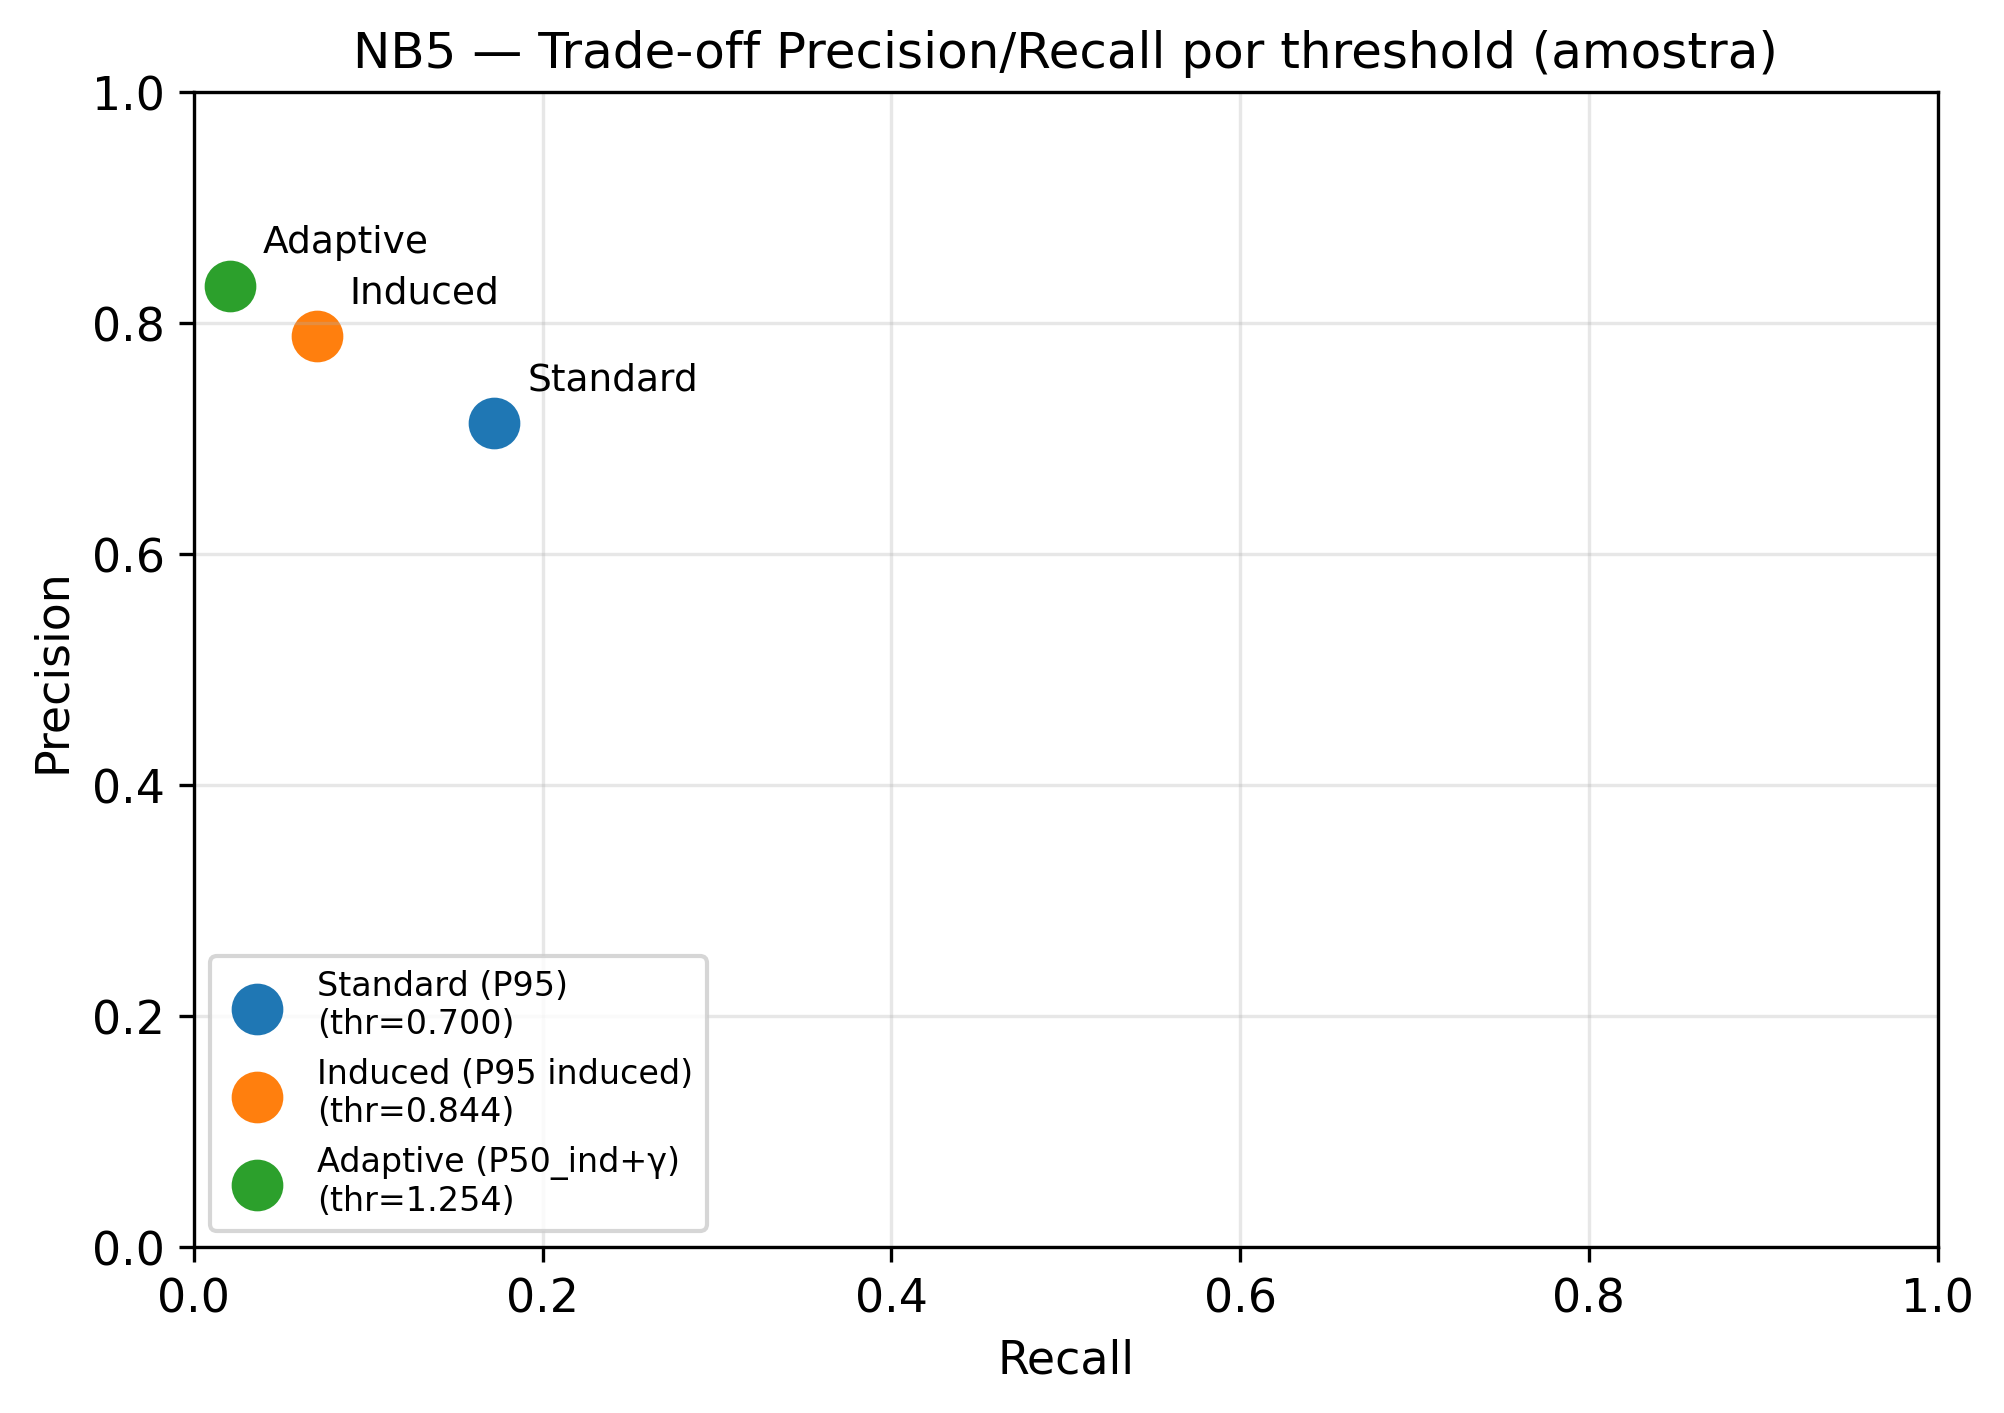
\includegraphics[width=0.7\textwidth]{figs/geradas/nb5_tradeoff_precision_recall.png}
    \caption{NB5 --- trade-off \emph{precision}/\emph{recall} entre os três thresholds.}
    \label{fig:nb5_tradeoff}
\end{figure}

\begin{figure}[!ht]
    \centering
    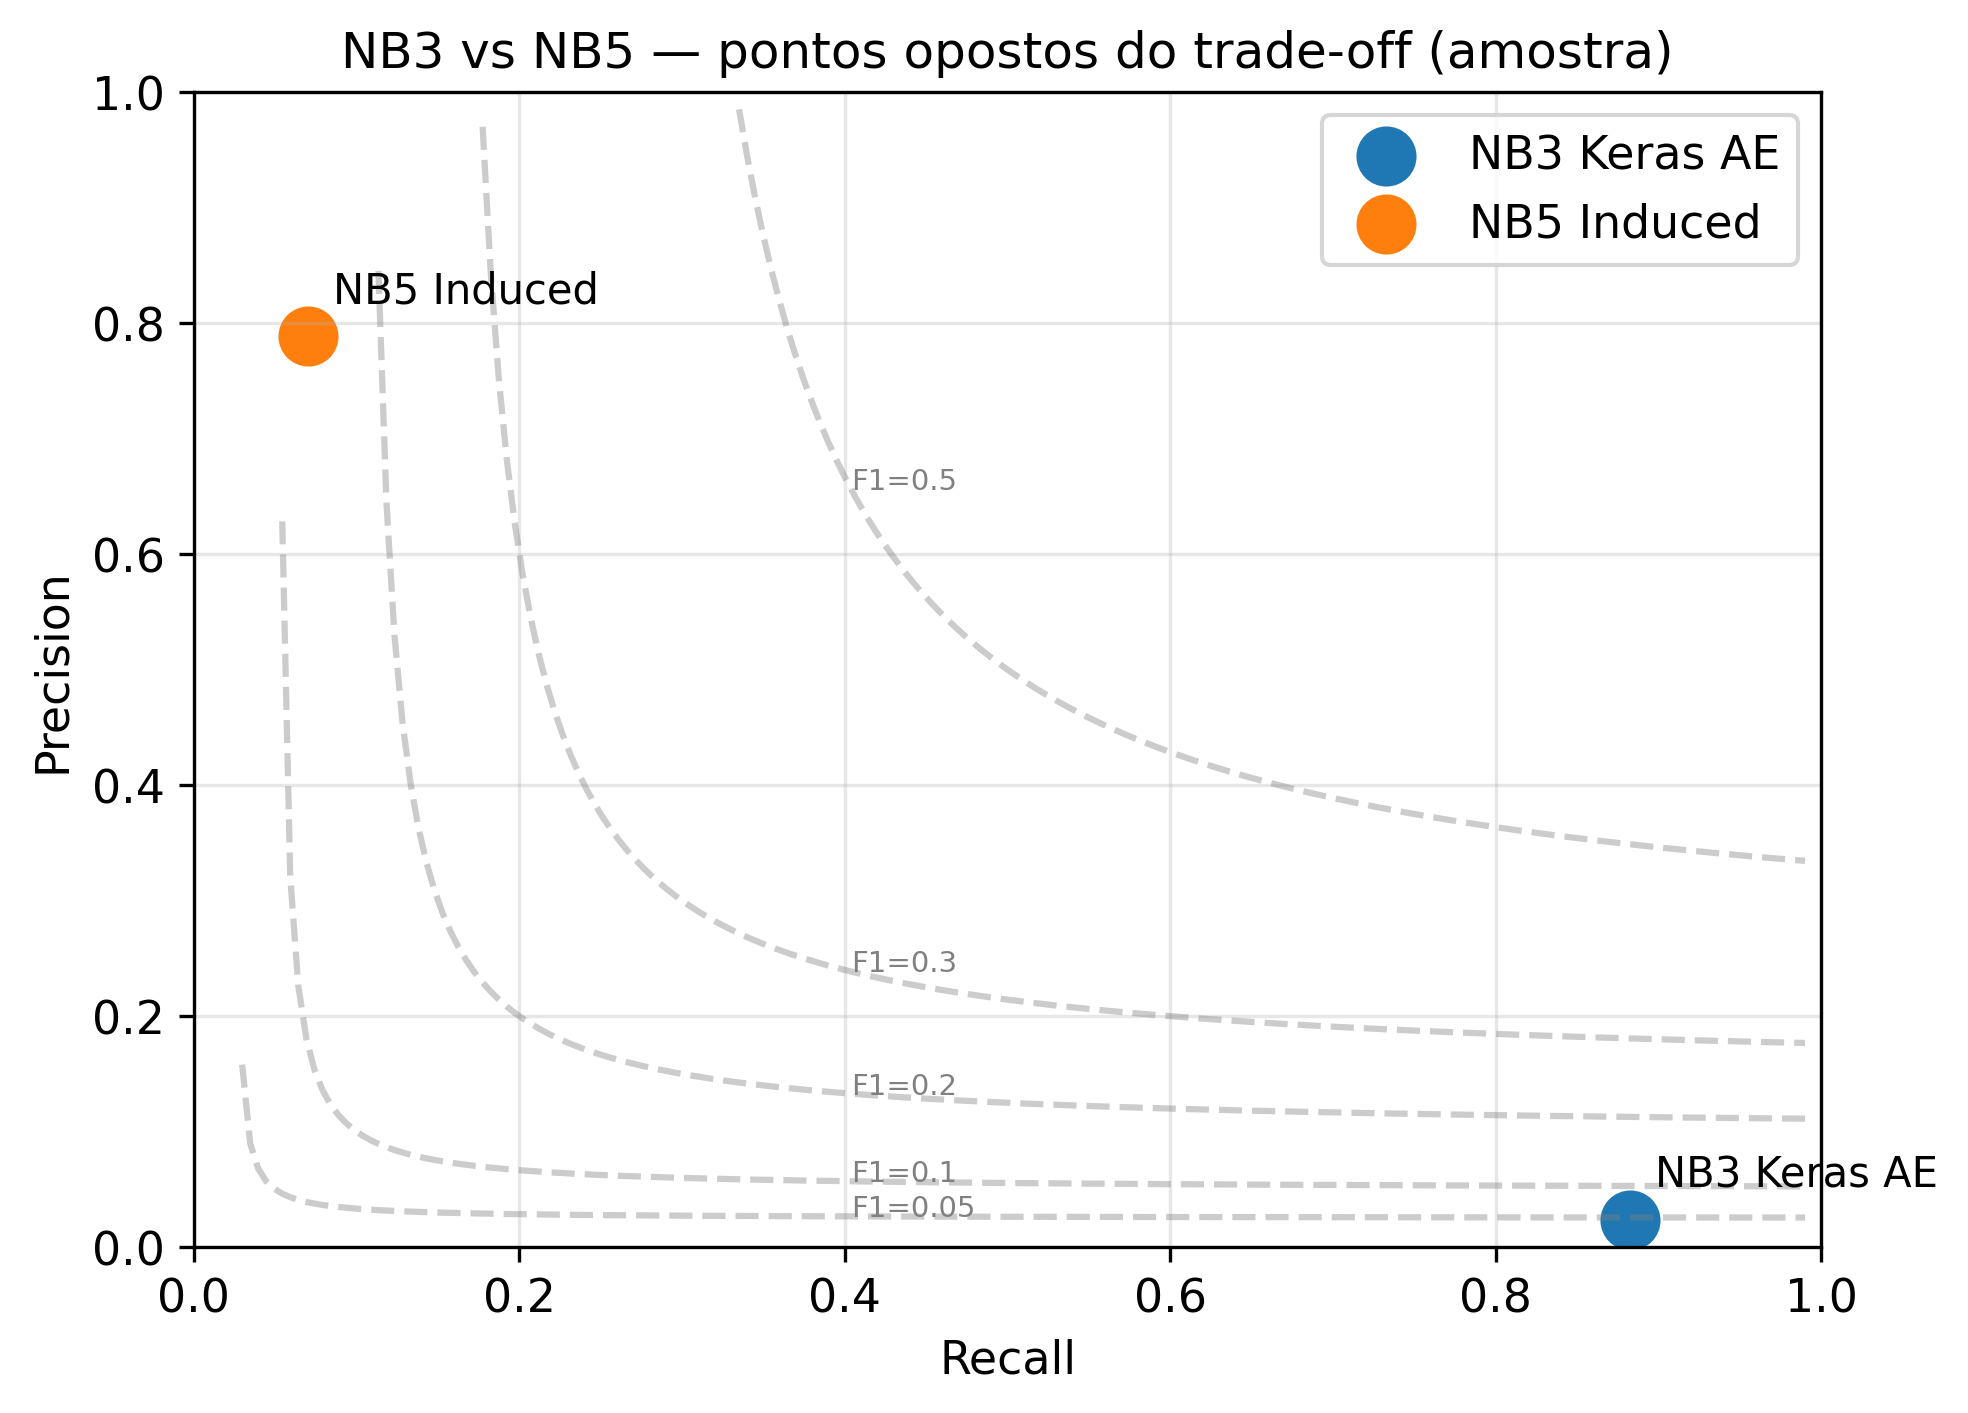
\includegraphics[width=0.7\textwidth]{figs/geradas/nb3_vs_nb5.png}
    \caption{NB3 vs NB5 ocupam pontos opostos do trade-off \emph{precision/recall}.}
    \label{fig:nb3_vs_nb5}
\end{figure}

Os artefatos qualitativos já gerados pelos próprios notebooks também são reproduzidos: ranking de importância XGBoost (Figura~\ref{fig:xgb_imp}), análise por feature do NB2 (Figura~\ref{fig:feat_anal}), curvas ROC/PR do NB2 (Figura~\ref{fig:roc_pr_nb2}), comparação induzido $\times$ baseline do NB4 (Figura~\ref{fig:nb4_comp}) e comparação de thresholds do NB5 (Figura~\ref{fig:nb5_comp}).

\begin{figure}[!ht]
    \centering
    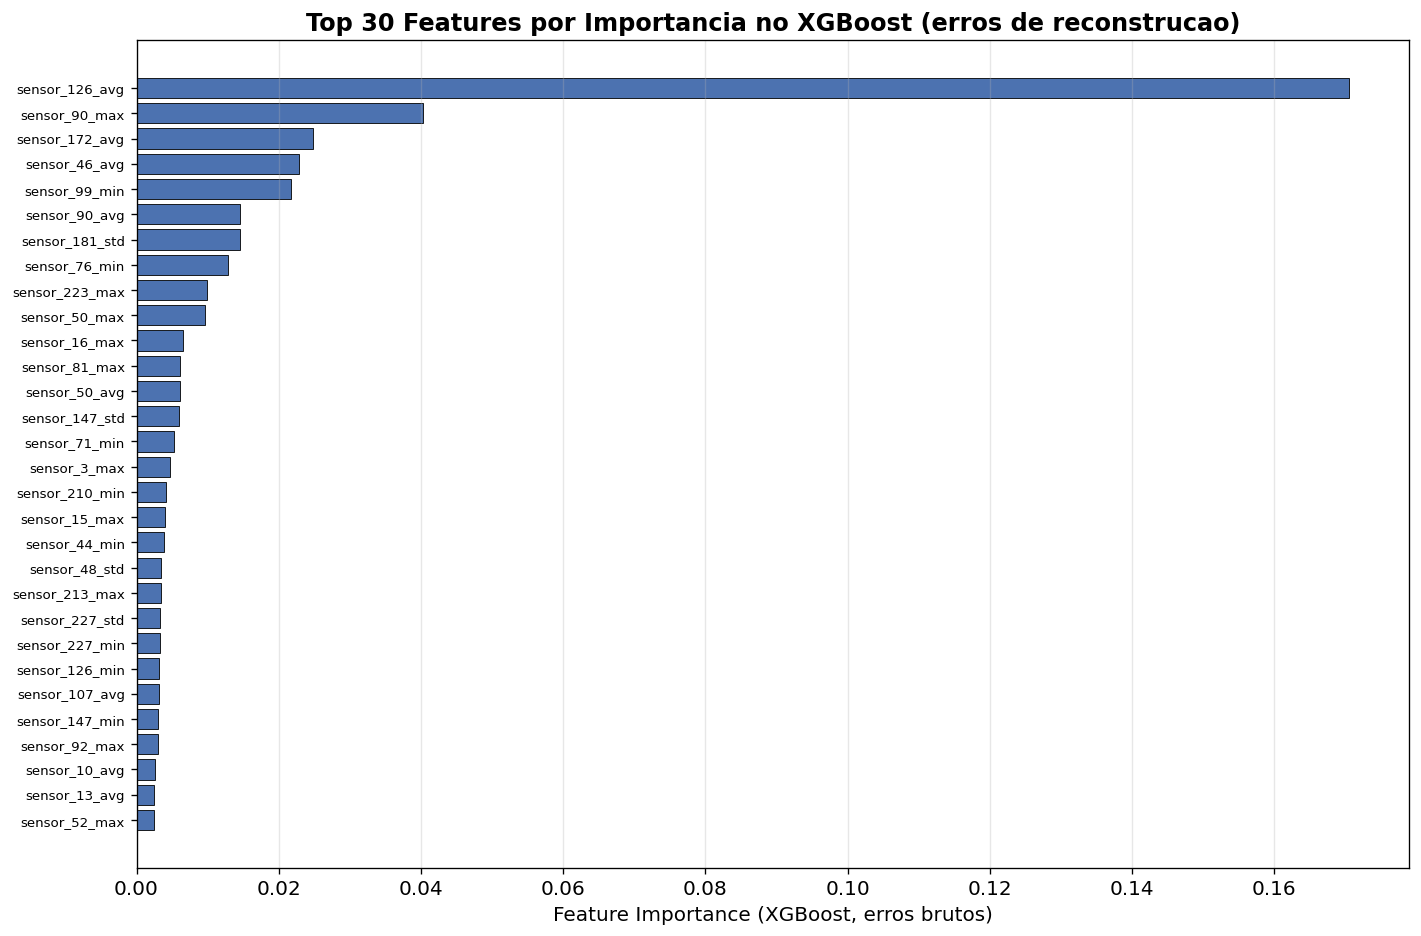
\includegraphics[width=0.85\textwidth]{resultados/02_cnn_bilstm_autoencoder/xgb_feature_importance.png}
    \caption{Ranking de importância das \emph{features} produzido pelo XGBoost (NB2).}
    \label{fig:xgb_imp}
\end{figure}

\begin{figure}[!ht]
    \centering
    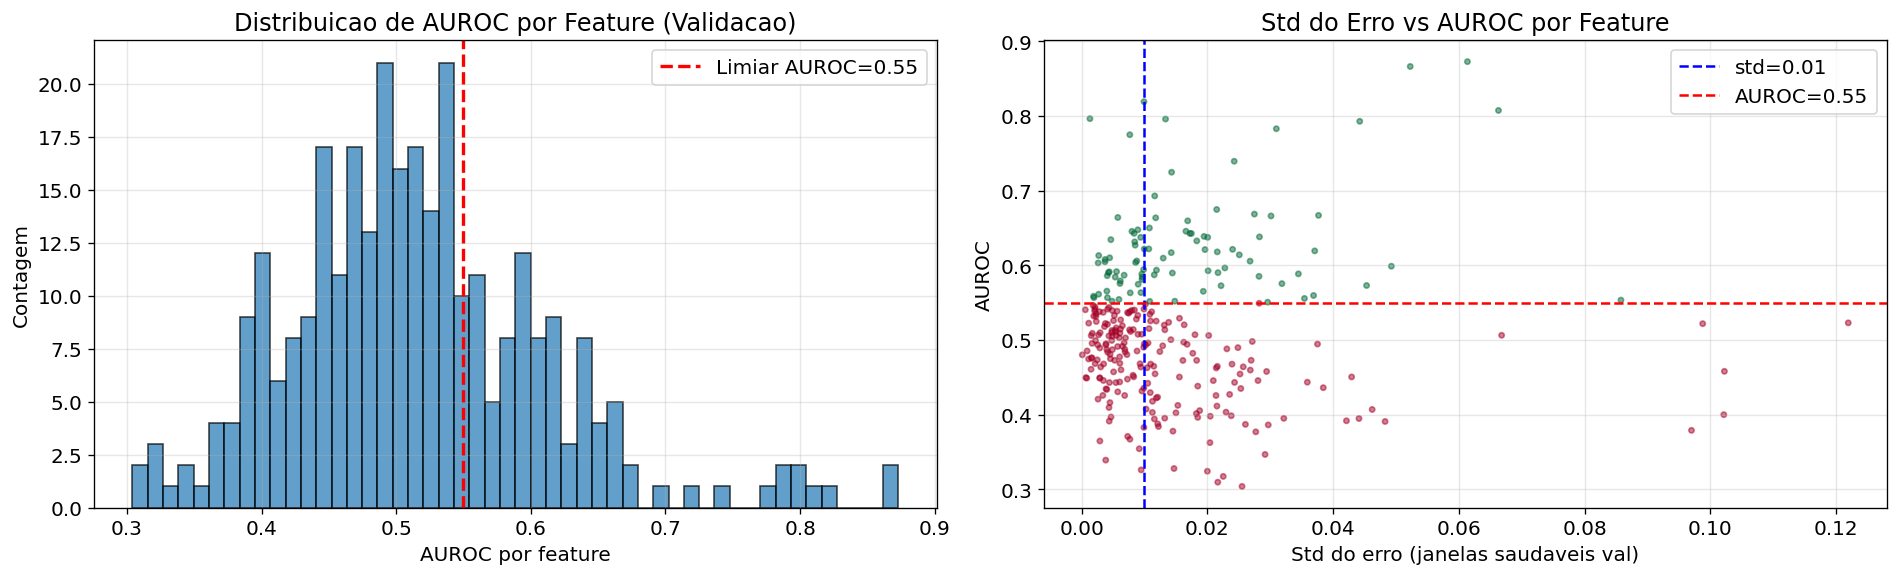
\includegraphics[width=0.95\textwidth]{resultados/02_cnn_bilstm_autoencoder/feature_analysis.png}
    \caption{Análise por feature (AUROC do erro de reconstrução --- NB2).}
    \label{fig:feat_anal}
\end{figure}

\begin{figure}[!ht]
    \centering
    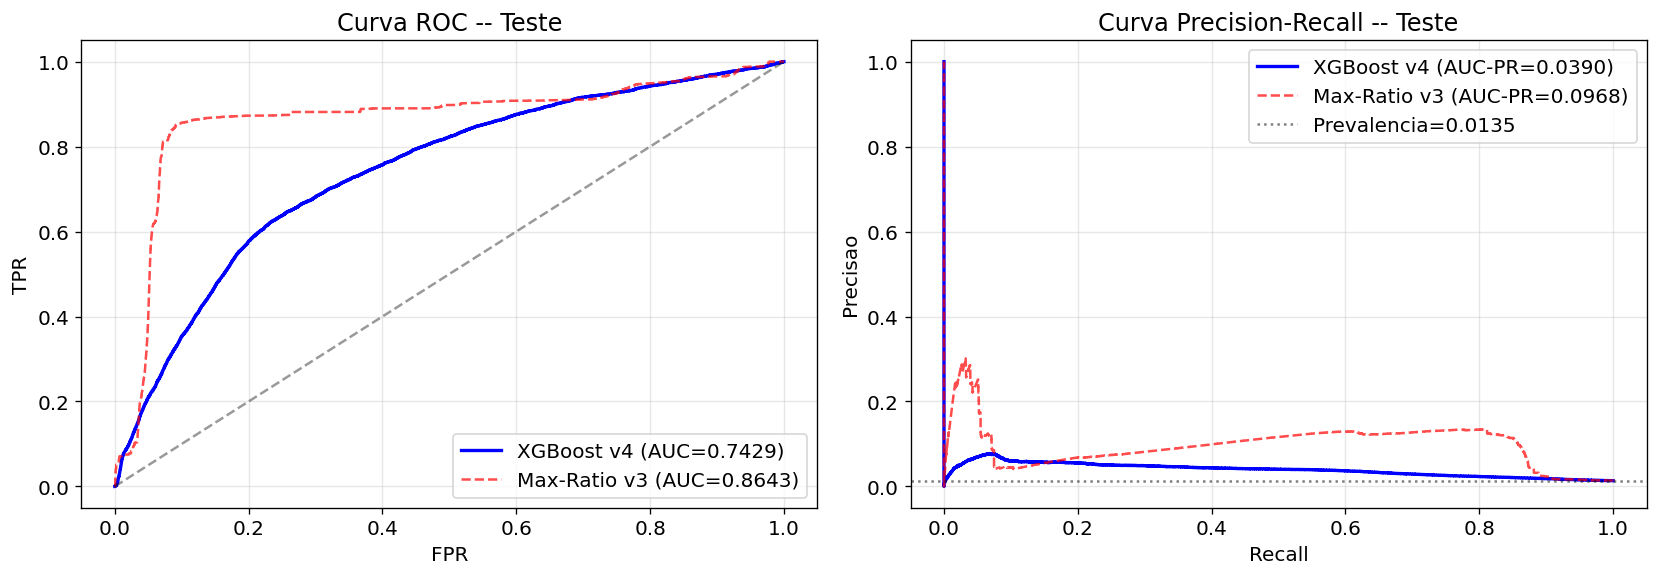
\includegraphics[width=0.95\textwidth]{resultados/02_cnn_bilstm_autoencoder/roc_pr_curves.png}
    \caption{Curvas ROC e Precision-Recall do NB2.}
    \label{fig:roc_pr_nb2}
\end{figure}

\begin{figure}[!ht]
    \centering
    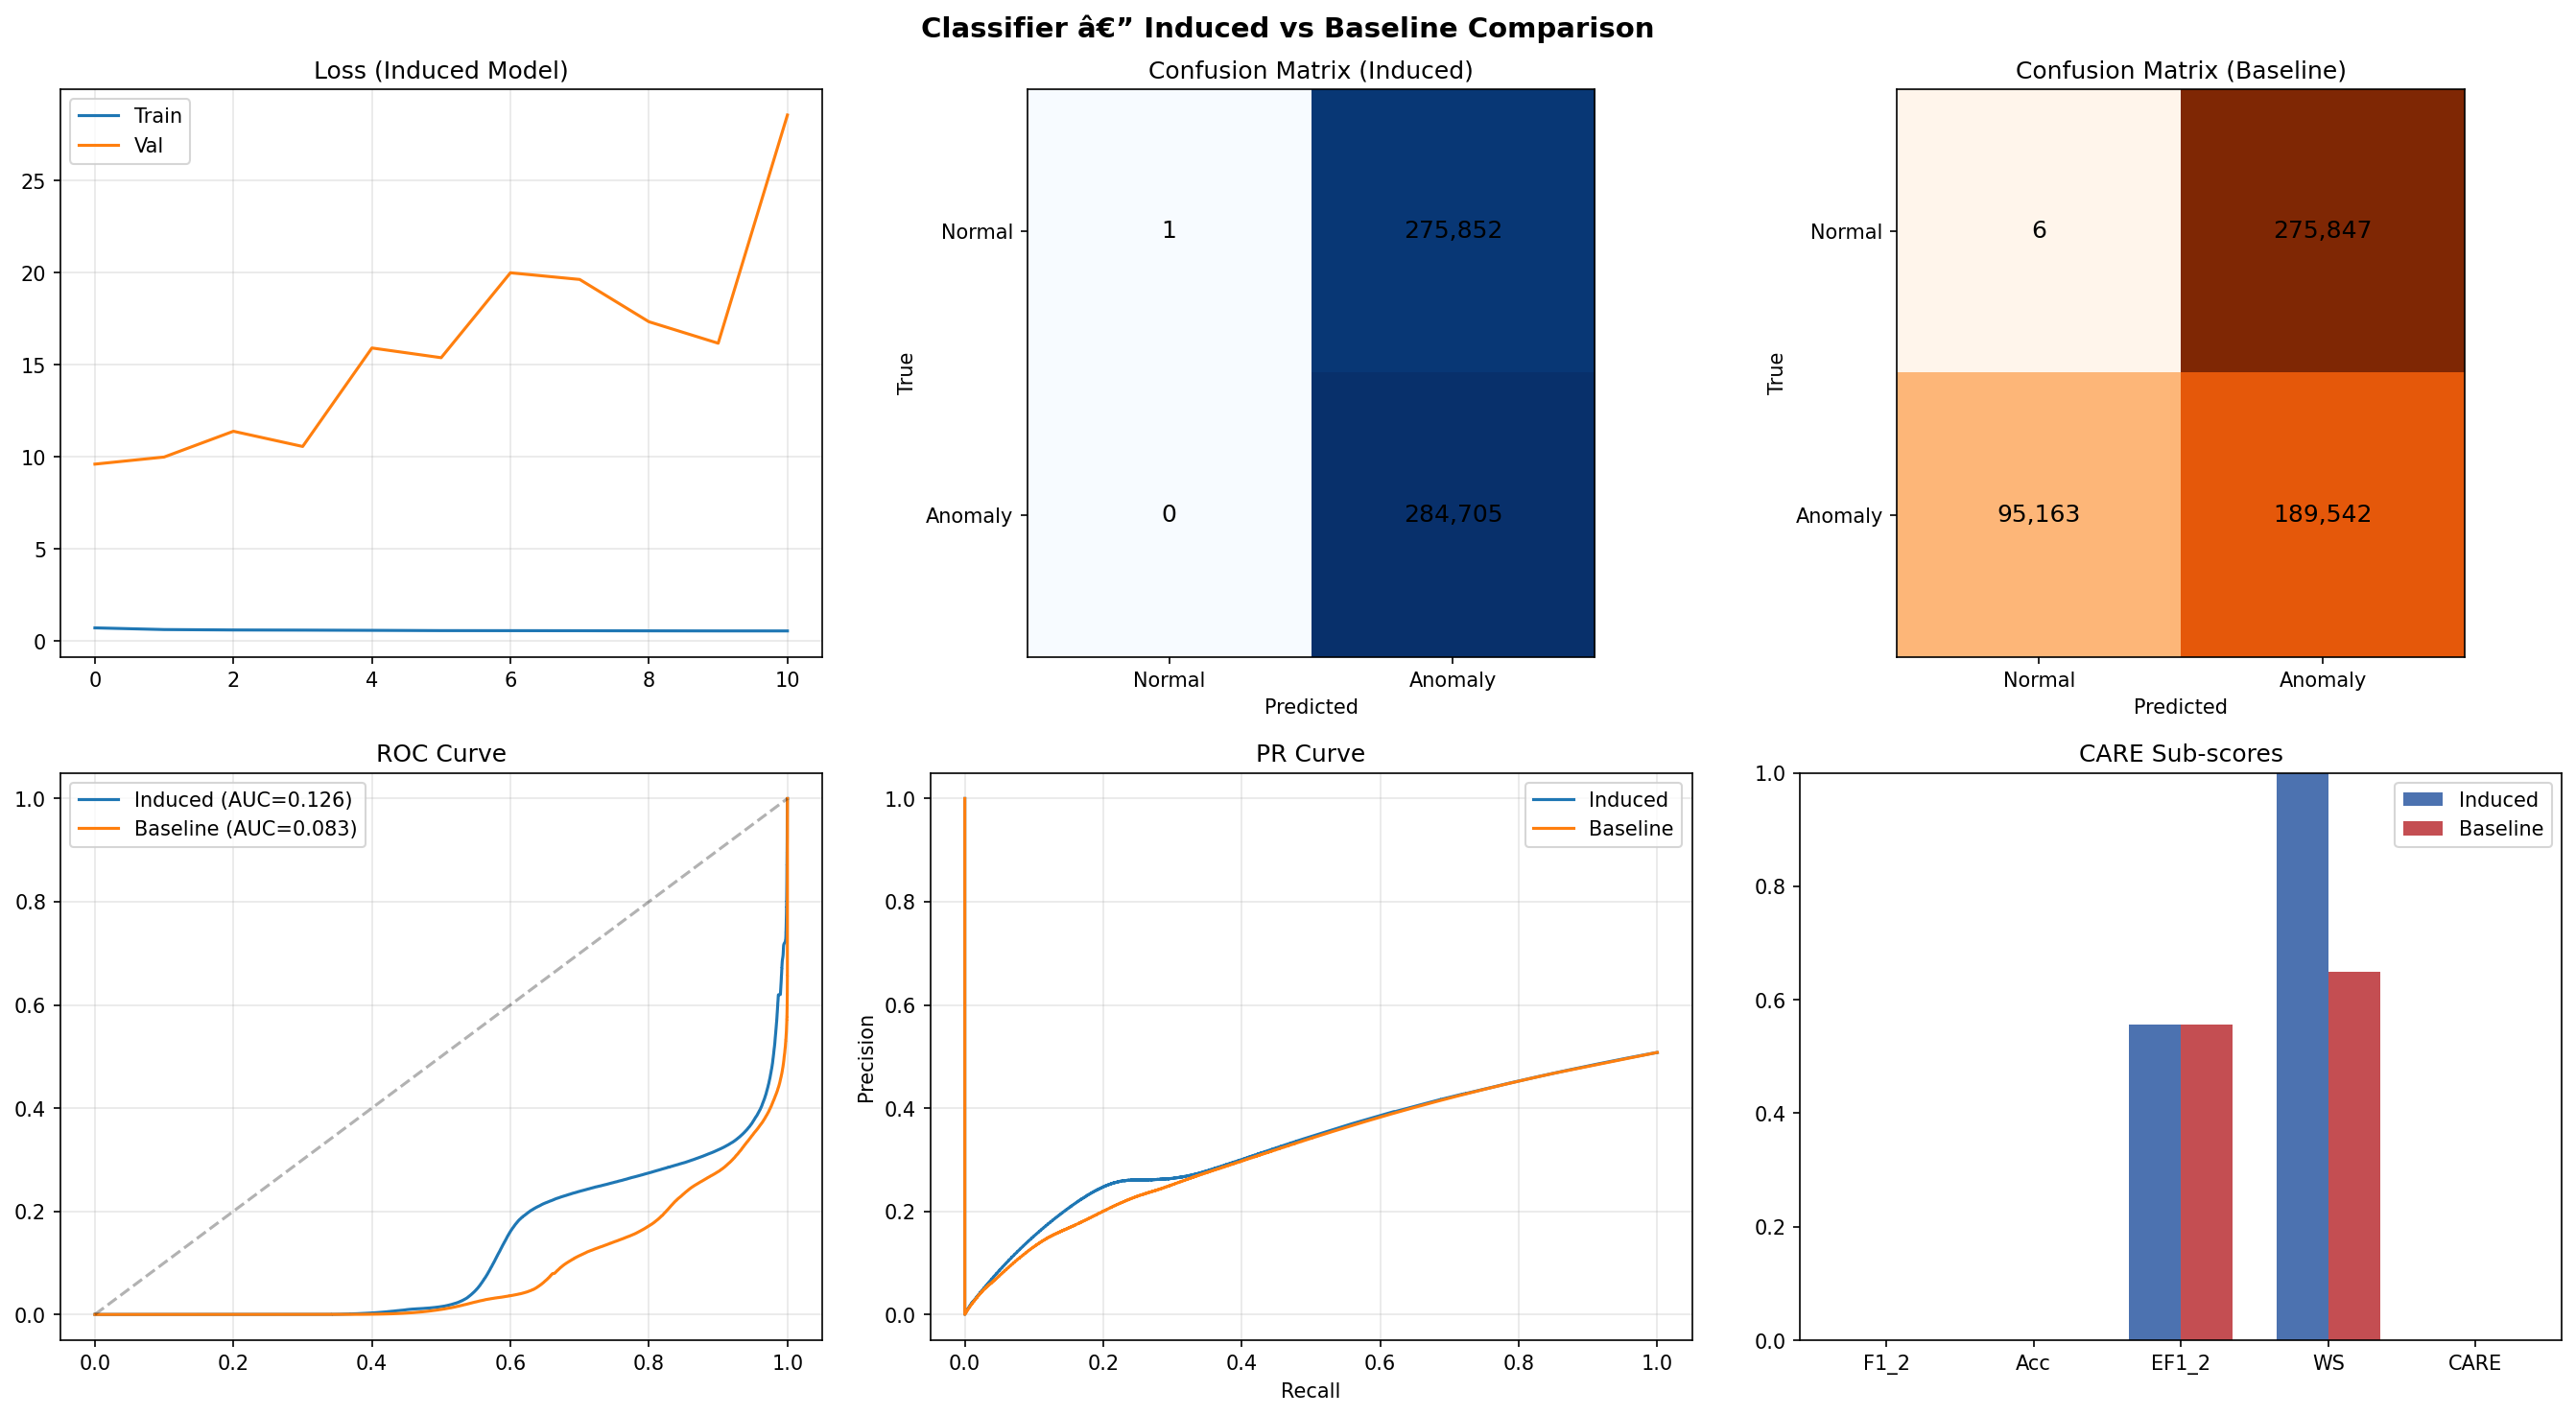
\includegraphics[width=0.95\textwidth]{resultados/04_classifier_induced_failure/comparison_plots.png}
    \caption{NB4 --- comparativo Modelo Induzido vs Baseline (loss, matrizes, ROC, PR, CARE).}
    \label{fig:nb4_comp}
\end{figure}

\begin{figure}[!ht]
    \centering
    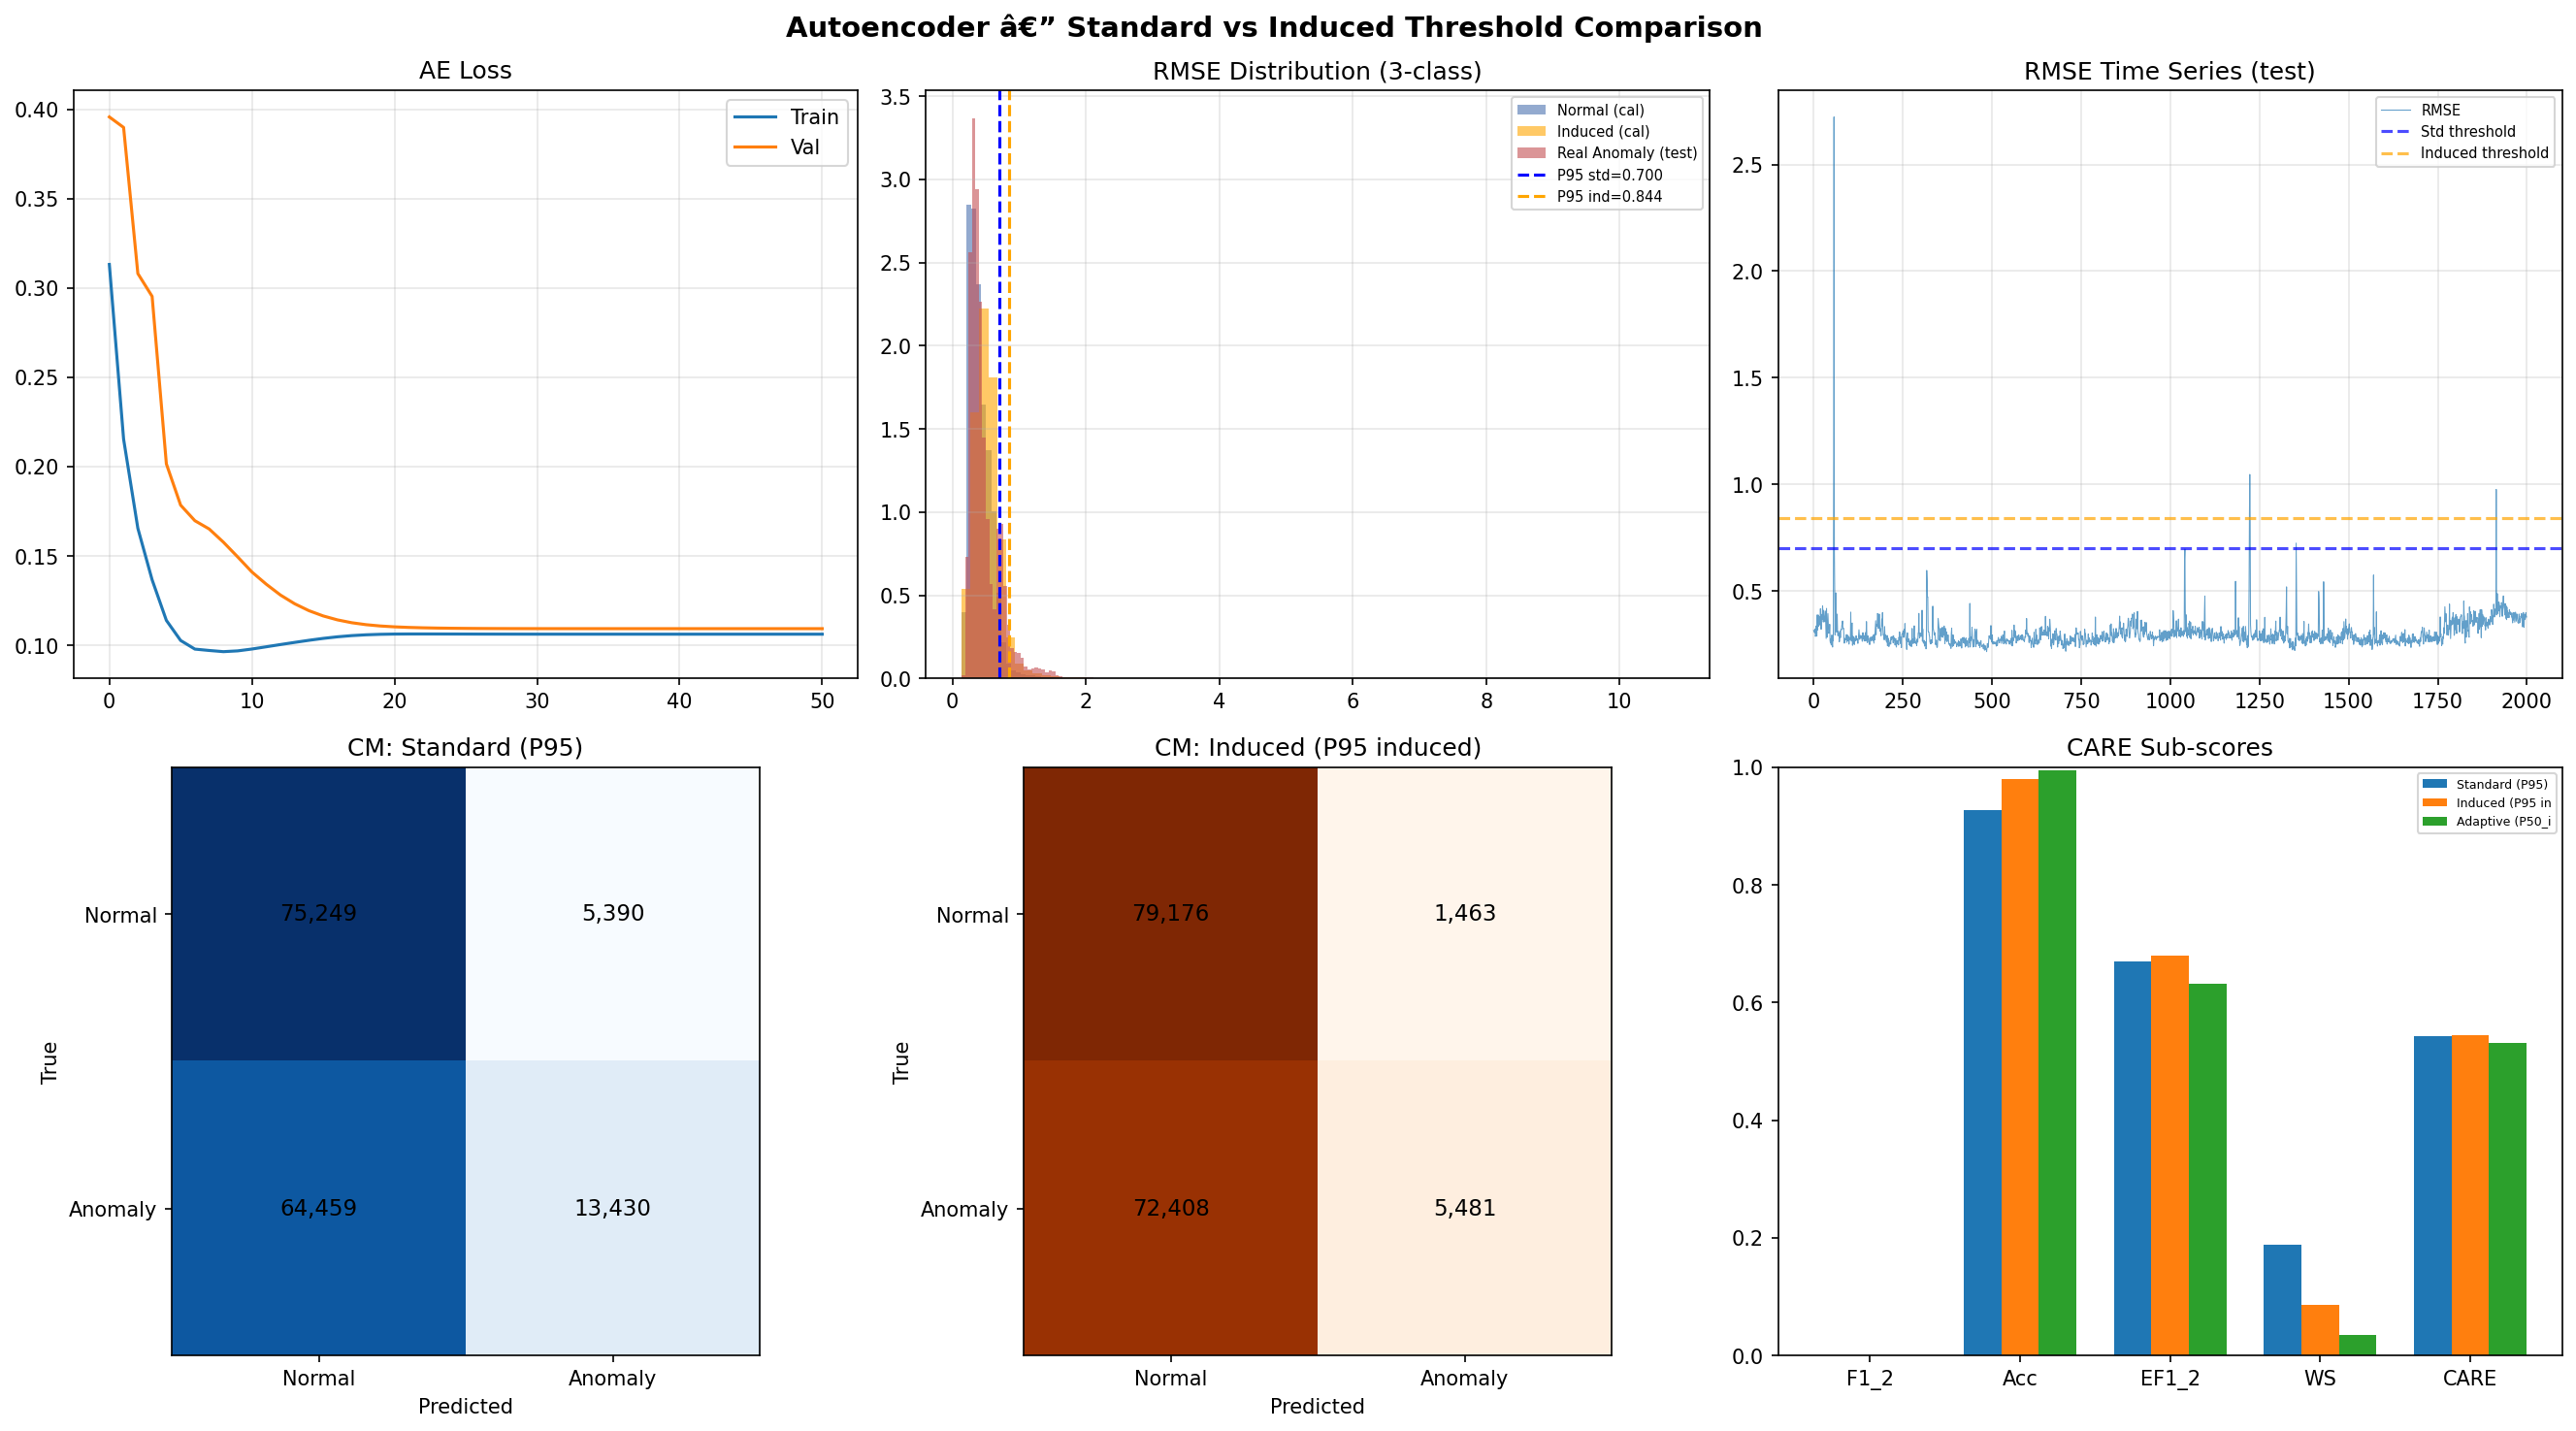
\includegraphics[width=0.95\textwidth]{resultados/05_autoencoder_induced_failure/comparison_plots.png}
    \caption{NB5 --- loss do AE, distribuição RMSE, série temporal e CARE para os três thresholds.}
    \label{fig:nb5_comp}
\end{figure}

\subsection{Discussão dos Resultados}

A leitura conjunta dos resultados quantitativos e qualitativos sustenta seis conclusões principais. (1) A \textbf{abordagem não supervisionada (autoencoders) supera a supervisionada} no contexto deste dataset severamente desbalanceado --- AUC-ROC chega a 0,872 no NB2 contra 0,66 do melhor supervisionado (NB1 CNN-LSTM); o NB3, embora avaliado apenas no padrão CARE (sem AUC-ROC amostral), atinge $EF1_2$=0,899 e CARE=0,699. (2) O \textbf{LSTM isolado falha completamente} ($F_1=0$, AUC=0,40) por colapso para a classe majoritária após o \textit{undersampling} 1:1 do treino encontrar a distribuição natural 58:1 no teste; este modelo não deve ser utilizado sem mecanismos robustos de balanceamento. (3) A \textbf{precisão amostral baixa ($\sim$2--3\%)} é o maior desafio aberto --- inviabiliza uso direto em produção pelo volume de falsos alarmes. (4) A \textbf{avaliação por evento é mais útil operacionalmente}: o NB3 atinge 94,1\% de \textit{recall} por dataset e 88,9\% de \textit{precision} por dataset (matriz de confusão 48 TP / 3 FN / 6 FP / 1 TN sobre 51 anômalos $+$ 7 normais), traduzindo-se em $EF1_2$=0,899 mesmo com $F1_2$ amostral de 0,393. (5) O \textbf{NB4 (classificador 3-classes com falhas induzidas) é operacionalmente inviável} apesar de apresentar o maior $F_1$ amostral (0,674) e \textit{recall} perfeito (1,000): seu CARE Score é $\approx$3,6$\times$10$^{-6}$ porque o modelo dispara alarme em \textbf{todos} os 5 eventos normais do split de teste (10 datasets: 5 anômalos $+$ 5 normais) --- Acc por evento normal $\approx$ 0 (qualquer classificador que sempre alarma obtém \textit{recall} 100\% ao custo de CARE $\approx$ 0). Esse resultado demonstra que métricas amostrais isoladas podem ser enganosas e que o CARE Score, ao incorporar especificidade por evento normal, expõe o colapso operacional que o $F_1$ amostral não revela. (6) A \textbf{calibração via falhas induzidas (NB5)} produz o ponto oposto da curva ROC em relação ao NB3 (alta \textit{precision} amostral, baixo \textit{recall}, mas alta especificidade por evento normal --- Acc=0,98), motivando \textit{ensemble} como linha de pesquisa imediata.

% ─── 11 LIMITAÇÕES DO ESTUDO ─────────────────────────────────────────────────
\section{Limitações do Estudo e Atribuições}\label{sec:limitacoes}

\subsection{Desvios em Relação ao Plano Original}

\begin{sloppypar}
Itens previstos no plano FAPESP que \textbf{não} foram realizados na forma originalmente proposta: (i) \textbf{arquitetura Transformer completa} --- apenas a camada \texttt{MultiHeadAttention} foi utilizada dentro do encoder CNN-BiLSTM (NB2), sem \textit{positional encoding} explícito nem blocos \textit{encoder/decoder} no padrão de \citet{Vaswani2017}; (ii) \textbf{integração com dados meteorológicos exógenos} (CPTEC/INPE, OpenWeatherMap) --- inviável devido à anonimização total do dataset CARE\_To\_Compare; (iii) \textbf{comparação direta ``modelos com vs.\ sem dados exógenos''} --- substituída pela comparação entre paradigmas (supervisionado vs.\ não supervisionado) e pela exploração de falhas induzidas como \textit{data augmentation}.
\end{sloppypar}

\subsection{Componentes Replicados de Fontes Externas}

\begin{sloppypar}
Os seguintes componentes foram adotados/replicados de repositórios externos e \textbf{não constituem contribuição original deste trabalho}: (i) framework \textbf{CARE Score} (Composite Anomaly Reliability Evaluation); (ii) análise \textbf{ARCANA} (importância de \textit{features} via reconstrução). Fonte: repositório público EnergyFaultDetector (AEFDI), \url{https://github.com/AEFDI/EnergyFaultDetector}. Esses módulos foram utilizados como ferramentas de avaliação padronizadas para permitir comparação com a literatura. Adicionalmente, a arquitetura CNN-LSTM do NB1 é uma \textbf{replicação} de \citet{Qi2024_CNN_LSTM_Energies}, adaptada para o cenário binário do CARE\_To\_Compare.
\end{sloppypar}

\subsection{Outras Limitações}

(i) \textbf{Escopo restrito ao Wind Farm C} --- generalização para outros parques (incluindo Wind Farm A e B do mesmo dataset) não foi avaliada. (ii) \textbf{Precisão amostral baixa ($\sim$2--3\%)} inviabiliza uso direto em produção sem etapas adicionais de filtragem ou \textit{ensemble}. (iii) \textbf{Hardware} --- treinamentos finais foram executados em GPU A6000 do laboratório; sem GPU dedicada, a reprodução completa do pipeline (Optuna $+$ cinco \textit{notebooks} $+$ CARE) é impraticável (Seções~6.1 e 8.3). (iv) \textbf{Avaliação restrita a janelas/amostras de SCADA} --- não foram analisados sinais de vibração de alta frequência ou imagens de termografia, que poderiam complementar o diagnóstico.

% ─── 12 CRONOGRAMA REALIZADO ─────────────────────────────────────────────────
\section{Cronograma Realizado vs Planejado}

A Tabela~\ref{tab:cronograma_real} compara as atividades A1--A9 do plano original com o executado durante o período da IC (06/2025--05/2026, vigência da bolsa FAPESP).

\begin{table}[!ht]
\centering
\small
\resizebox{\linewidth}{!}{%
\begin{tabular}{l|l|p{7cm}}
\hline
\textbf{Atividade} & \textbf{Status} & \textbf{Observações} \\
\hline
A1 (Literatura)              & Concluído (contínuo) & Mantido ao longo de toda a IC. \\
A2 (ML básico)               & Concluído            & Curso externo + exercícios PyTorch. \\
A3 (Pré-proc / Modelos)      & Concluído            & LSTM/CNN/Atenção estudados; Transformer completo não implementado. \\
A4 (Coleta / Pré-proc)       & Concluído (parcial)  & SCADA OK; meteorológicos inviáveis pela anonimização. \\
A5 (Treino sem exógenos)     & Concluído            & Cinco notebooks executados. \\
A6 (Treino com exógenos)     & Cancelado            & Substituído por NB4/NB5 (falhas induzidas). \\
A7 (Avaliação / Comparação)  & Concluído            & Métricas amostrais e CARE consolidados. \\
A8 (Análise / Interpretação) & Concluído            & Discussão e ablação documentadas. \\
A9 (Relatórios)              & Concluído            & Relatório final entregue à FAPESP. \\
\hline
\end{tabular}%
}
\caption{Cronograma realizado vs.\ planejado (A1--A9 do plano FAPESP).}
\label{tab:cronograma_real}
\end{table}

% ─── 13 MATÉRIAS CURSADAS NA FACULDADE ───────────────────────────────────────
\section{Matérias Cursadas na Faculdade}

A Tabela~\ref{tab:disciplinas} relaciona as disciplinas cursadas durante o período de vigência da IC e sua contribuição para o projeto.

\begin{table}[!ht]
\centering
\small
\resizebox{\linewidth}{!}{%
\begin{tabular}{l|c|p{5.5cm}}
\hline
\textbf{Disciplina} & \textbf{Semestre} & \textbf{Relação com o projeto} \\
\hline
Fenômenos Eletromagnéticos                                                & 2025.2 & Base física para sensores SCADA (corrente, tensão, campo). \\
Prática em Projetos Extensionistas II                                     & 2025.2 & Metodologia de projetos aplicados. \\
Programação Orientada a Objetos                                           & 2025.2 & Modelagem dos pipelines de pré-processamento e modelos. \\
Lab.\ Sist.\ Computacionais: Circuitos Digitais                           & 2025.2 & Fundamentos de hardware digital. \\
Arquitetura e Organização de Computadores                                 & 2025.2 & Compreensão da execução em GPU/TPU. \\
Circuitos Elétricos I                                                     & 2025.2 & Análise de variáveis elétricas das turbinas. \\
Projeto e Análise de Algoritmos                                           & 2025.2 & Complexidade de algoritmos de seleção de \textit{features}. \\
Análise de Sinais                                                         & 2026.1 & Tratamento de séries temporais SCADA, FFT, filtros. \\
Circuitos Elétricos II                                                    & 2026.1 & Análise de regimes transitórios e CA. \\
Introdução aos Materiais Elétricos                                        & 2026.1 & Materiais de geradores e conversores. \\
Lab.\ Sist.\ Computacionais: Arq.\ e Org.\ de Computadores                & 2026.1 & Prática de execução em hardware especializado. \\
Linguagens Formais e Autômatos                                            & 2026.1 & Base teórica para máquinas de estado e parsing. \\
Algoritmos em Bioinformática                                              & 2026.1 & Análise de sequências e distâncias --- raciocínio algorítmico complementar ao projeto (disciplina obrigatória do currículo). \\
Fenômenos Eletromagnéticos Experimental                                   & 2026.1 & Prática laboratorial complementar. \\
\hline
\end{tabular}%
}
\caption{Disciplinas cursadas durante a vigência da IC (2025.2 e 2026.1).}
\label{tab:disciplinas}
\end{table}

% ─── 16 LIÇÕES APRENDIDAS ────────────────────────────────────────────────────
\section{Lições Aprendidas}

(1) \textbf{Métricas importam mais que modelos} no cenário desbalanceado --- a escolha de $F_1$, AUC-ROC e CARE em vez de acurácia muda fundamentalmente a interpretação dos resultados. (2) \textbf{Pipeline antes de modelo} --- bugs no pré-processamento (e.g., \textit{leakage} do scaler ajustado em validação) podem esconder ou inflar resultados; a separação rígida treino/validação/teste e a fixação de \textit{seeds} são pré-requisitos. (3) \textbf{Replicar antes de inovar} --- a replicação do paper de \citet{Qi2024_CNN_LSTM_Energies} (NB1) revelou limitações práticas (colapso do LSTM) que motivaram a migração para o paradigma não supervisionado. (4) \textbf{Hardware é restrição real} --- a expectativa inicial de treinar tudo em CPU foi rapidamente abandonada; o uso de GPU passou de ``conveniência'' a pré-requisito. (5) \textbf{Anonimização de dados públicos} é uma limitação não discutida na maioria dos papers, mas que pode inviabilizar inteiras linhas de pesquisa --- motivou o redirecionamento do escopo deste projeto.

% ─── 17 TRABALHOS FUTUROS ────────────────────────────────────────────────────
\section{Trabalhos Futuros}\label{sec:trabalhos-futuros}

Desdobramentos naturais deste trabalho incluem: (1) \textbf{Ensemble NB3 + NB5}, combinando o alto \textit{recall} amostral do NB3 com a alta especificidade por evento do NB5, potencialmente atingindo um ponto operacional intermediário viável em produção. (2) \textbf{Focal Loss} no NB1 para mitigar o colapso do LSTM e melhorar o tratamento do desbalanceamento. (3) \textbf{Threshold por regime operacional} (partida, geração nominal, parada), reduzindo falsos positivos causados por variações legítimas. (4) \textbf{Generalização cross-farm} --- avaliar os modelos do Wind Farm C nos Wind Farms A e B com técnicas de \textit{domain adaptation}. (5) \textbf{Implementação de Transformer completo} (com \textit{positional encoding} e blocos \textit{encoder/decoder}) para fechar o item pendente do plano original.

% ─── 18 CONSIDERAÇÕES FINAIS ─────────────────────────────────────────────────
\section{Considerações Finais}

Este relatório documenta os principais resultados obtidos na Iniciação Científica em detecção de anomalias em turbinas eólicas. Apesar da inviabilidade técnica de integrar dados meteorológicos exógenos --- inicialmente o foco central do plano FAPESP ---, o projeto se readequou produtivamente para a comparação entre paradigmas de detecção e a exploração de falhas induzidas como técnica de \textit{data augmentation}. Os autoencoders não supervisionados se mostraram superiores aos modelos supervisionados sob desbalanceamento severo (AUC-ROC 0,87 vs.\ 0,66), e a calibração de \textit{thresholds} via falhas sintéticas abriu uma linha de pesquisa promissora pela alta especificidade por evento que produz. A contribuição formativa para o aluno foi significativa, abrangendo desde os fundamentos de aprendizado profundo até pipelines de produção em PyTorch e Keras, otimização automática com Optuna e integração com frameworks de avaliação padronizados (CARE Score / EnergyFaultDetector). Todos os notebooks, experimentos, pipelines e resultados estão disponíveis publicamente no repositório GitHub do projeto: \url{https://github.com/Thiago-Heleno/IC_Thiago-Heleno_Wind_Turbines}.

% ─── REFERÊNCIAS ─────────────────────────────────────────────────────────────
\nocite{*}
\bibliographystyle{plainnat}
\bibliography{referencias}

\end{document}